\documentclass[a4j,12pt]{jarticle}
\usepackage[demo]{mmda}
% \usepackage{mmda}% to enable figure inclusion
%
\title{CCSR/NIES AGCM Document}
\date{1995/01/19}
% \Dnofoot
\def\Module#1{{[\tt #1]}}
% \Dparindent

% \includeonly{p-lsc}
% \includeonly{dynamics}
% \includeonly{physics}
%
%\makeindex

\begin{document}
%
\pagenumbering{roman}
\title{\Huge CCSR/NIES AGCM の解説}
\author{}
\date{1995年1月19日}
\maketitle
\tableofcontents
\clearpage
\pagenumbering{arabic}

%
% ccsr/nies agcm の特徴の list
\hypertarget{model-overview.}{%
\section{Model Overview.}\label{model-overview.}}

\hypertarget{characteristics-of-ccsrnies-agcm}{%
\subsection{Characteristics of CCSR/NIES
AGCM}\label{characteristics-of-ccsrnies-agcm}}

AGCM5.4 was developed in collaboration with the Center for Climate
System Research (CCSR) at the University of Tokyo. Prepared in
collaboration with the National Institute for Environmental Studies
(NIES) , The model is a global three-dimensional general circulation
model. The features of the model are listed below.

\begin{longtable}[]{@{}ll@{}}
\toprule
\begin{minipage}[b]{0.47\columnwidth}\raggedright
Header0\strut
\end{minipage} & \begin{minipage}[b]{0.47\columnwidth}\raggedright
Header1\strut
\end{minipage}\tabularnewline
\midrule
\endhead
\begin{minipage}[t]{0.47\columnwidth}\raggedright
System of equations\strut
\end{minipage} & \begin{minipage}[t]{0.47\columnwidth}\raggedright
System of hydrostatic primitive equations\strut
\end{minipage}\tabularnewline
\begin{minipage}[t]{0.47\columnwidth}\raggedright
Area.\strut
\end{minipage} & \begin{minipage}[t]{0.47\columnwidth}\raggedright
Global 3D\strut
\end{minipage}\tabularnewline
\begin{minipage}[t]{0.47\columnwidth}\raggedright
Predictive variables\strut
\end{minipage} & \begin{minipage}[t]{0.47\columnwidth}\raggedright
\strut
\end{minipage}\tabularnewline
\begin{minipage}[t]{0.47\columnwidth}\raggedright
Horizontal Discretization\strut
\end{minipage} & \begin{minipage}[t]{0.47\columnwidth}\raggedright
Spectral Conversion Method\strut
\end{minipage}\tabularnewline
\begin{minipage}[t]{0.47\columnwidth}\raggedright
Vertical discretization\strut
\end{minipage} & \begin{minipage}[t]{0.47\columnwidth}\raggedright
σ system (Arakawa and Suarez, 1983)\strut
\end{minipage}\tabularnewline
\begin{minipage}[t]{0.47\columnwidth}\raggedright
Radiation\strut
\end{minipage} & \begin{minipage}[t]{0.47\columnwidth}\raggedright
2-stream DOM/adding method\strut
\end{minipage}\tabularnewline
\begin{minipage}[t]{0.47\columnwidth}\raggedright
\strut
\end{minipage} & \begin{minipage}[t]{0.47\columnwidth}\raggedright
(Based on Nakajima and Tanaka, 1986)\strut
\end{minipage}\tabularnewline
\begin{minipage}[t]{0.47\columnwidth}\raggedright
A large-scale cloud process\strut
\end{minipage} & \begin{minipage}[t]{0.47\columnwidth}\raggedright
Scheme with the total water mixing ratio as a forecast variable\strut
\end{minipage}\tabularnewline
\begin{minipage}[t]{0.47\columnwidth}\raggedright
\strut
\end{minipage} & \begin{minipage}[t]{0.47\columnwidth}\raggedright
(Based on Le Treut and Li, 1991)\strut
\end{minipage}\tabularnewline
\begin{minipage}[t]{0.47\columnwidth}\raggedright
Cumulus Convection\strut
\end{minipage} & \begin{minipage}[t]{0.47\columnwidth}\raggedright
Simplified Arakawa-Schubert scheme\strut
\end{minipage}\tabularnewline
\begin{minipage}[t]{0.47\columnwidth}\raggedright
Vertical Diffusion\strut
\end{minipage} & \begin{minipage}[t]{0.47\columnwidth}\raggedright
Mellor and Yamada(1974) level2\strut
\end{minipage}\tabularnewline
\begin{minipage}[t]{0.47\columnwidth}\raggedright
\strut
\end{minipage} & \begin{minipage}[t]{0.47\columnwidth}\raggedright
Louis (1979), bulk type\strut
\end{minipage}\tabularnewline
\begin{minipage}[t]{0.47\columnwidth}\raggedright
\strut
\end{minipage} & \begin{minipage}[t]{0.47\columnwidth}\raggedright
(Considering the convection effect of stomatal resistance, Miller et
al.~1992)\strut
\end{minipage}\tabularnewline
\begin{minipage}[t]{0.47\columnwidth}\raggedright
Surface Thermal Processes\strut
\end{minipage} & \begin{minipage}[t]{0.47\columnwidth}\raggedright
Multilayer Heat Transfer\strut
\end{minipage}\tabularnewline
\begin{minipage}[t]{0.47\columnwidth}\raggedright
Surface Hydrological Processes\strut
\end{minipage} & \begin{minipage}[t]{0.47\columnwidth}\raggedright
Bucket Model\strut
\end{minipage}\tabularnewline
\begin{minipage}[t]{0.47\columnwidth}\raggedright
\strut
\end{minipage} & \begin{minipage}[t]{0.47\columnwidth}\raggedright
\strut
\end{minipage}\tabularnewline
\begin{minipage}[t]{0.47\columnwidth}\raggedright
\strut
\end{minipage} & \begin{minipage}[t]{0.47\columnwidth}\raggedright
Scheme based on McFarlane (1987)\strut
\end{minipage}\tabularnewline
\begin{minipage}[t]{0.47\columnwidth}\raggedright
\strut
\end{minipage} & \begin{minipage}[t]{0.47\columnwidth}\raggedright
The north-south vertical and east-west vertical two-dimensional
models.\strut
\end{minipage}\tabularnewline
\bottomrule
\end{longtable}

\begin{verbatim}
The vertical one-dimensional model.
\end{verbatim}

\begin{itemize}
\item
  TAB00000: 18.0
\item
  TAB00000: 18.1\\
  The mixed-layer coupled model for the ocean
\end{itemize}

% agcm の概念と構造
\hypertarget{features-and-structure-of-the-model}{%
\subsection{Features and structure of the
model}\label{features-and-structure-of-the-model}}

\textbf{NOTE: the descriptions in this section are outdated.}

\hypertarget{basic-features-of-the-model.}{%
\subsubsection{Basic Features of the
Model.}\label{basic-features-of-the-model.}}

The MIROC6 AGCM is a numerical model for describing the global
three-dimensional atmosphere based on physical laws and calculating the
time evolution of the system as an initial value problem or a boundary
value problem.

The data to be inputted are as follows.

\begin{itemize}
\item
  Initial data for each prognostic variable (horizontal wind speed,
  temperature, surface pressure, specific humidity, cloud liquid water
  content, etc.)
\item
  Boundary condition data (surface elevation, surface condition, sea
  surface temperature, etc.)
\item
  Various parameters of the model (atmospheric components, physical
  process parameters, etc.)
\end{itemize}

On the other hand, the output is the following.

\begin{itemize}
\item
  Data for each prognostic parameter and diagnostic parameter, for each
  time or time average
\item
  Initial data to be used for continuous execution (restart data)
\item
  Progress and various diagnostic messages
\end{itemize}

The prognostic variable is the data obtained as a time series by
integrating the differential equation of time evolution, and the
diagnostic variable is the quantity calculated from the prognostic
variable, the boundary conditions and the parameters by some method that
does not include time integration.

More specifically, the model basically solves the following equations
(prognostic equations).

\begin{eqnarray}
  \frac{\partial{u}}{\partial {t}}  =  \left( {\mathcal F}_x \right)_D + \left( {\mathcal F}_x \right)_P.
   \\
  \frac{\partial{v}}{\partial {t}}  =  \left( {\mathcal F}_y \right)_D + \left( {\mathcal F}_y \right)_P. \\
  \frac{\partial{T}}{\partial {t}}  =  \left( Q \right)_D + \left( Q \right)_P. \\
  \frac{\partial{p_S}}{\partial {t}}  =  \left( M \right)_D + \left( M \right)_P. \\
  \frac{\partial{q}}{\partial {t}}  =  \left( S \right)_D + \left( S \right)_P. \\
  \frac{\partial{T_g}}{\partial {t}}  =  \left( Q_g \right)_D + \left( Q_g \right)_P.
\end{eqnarray}

Here, \(u,v,T,p_S,q,T_g\) are two-dimensional and three-dimensional
prognostic variables such as eastward wind, northward wind, temperature,
surface pressure, specific humidity, and surface state amount,
respectively, and the right-hand side is a term that causes time
variation of each prognostic variable. The terms
\({\mathcal F}_x,{\mathcal F}_y,Q,S,Q_g\) are calculated based on the
prognostic variables \(u,v,T,p_S,q,T_g\), are divided into two main
categories: the terms \(u\) and \(v\), such as advection due to the
motion of the atmosphere (the terms with index \(D\) in the above
equation), and the terms such as cloud and radiation (the terms with
index \(P\) in the above equation). There are two main types of terms.
The former is called the dynamical process, and the latter is called the
physical process.

The advection term is the main part of the time-varying term in
dynamical processes, and the accurate estimation of the spatial
derivative is important in its calculation. The MIROC6 AGCM utilizes the
spherical harmonic expansion to calculate the horizontal differential
term. On the other hand, it is important for physical processes to be
represented in a simple model with parameters (parameterization), such
as energy conversions due to the phase change of water, radiative
absorption and emission, the effects of small-scale atmospheric motions,
and the effects of various processes on the ground surface.

The time integration of the prognostic equation is done by approximating
the left-hand side of (1) etc. by the difference. For example,

\begin{eqnarray}
  \frac{\partial{q}}{\partial {t}} \rightarrow \frac{q^{t+\Delta t} - q^{t}}{\Delta t}
\end{eqnarray}

By making ,

\begin{eqnarray}
  q^{t+\Delta t} = q^{t}
       + \Delta t \left[ \left( S \right)_D + \left( S \right)_P  \right]
\end{eqnarray}

where \(S\) is a function of the prognostic variables \(u,v,T,p_S,q\).
Although \(S\) is a function of the prognostic variables
\(u,v,T,p_S,q\), and so on, there are various time difference schemes
that can be used in this calculation depending on the time of day the
prognostic variables are used to evaluate \(S\). The MIROC6 AGCM uses
the Euler method, which uses the value of the \(t\) as it is, the leap
frog method, which uses the value of the \(t+\Delta t/2\), and the
implicit method, which uses the (approximate) value of the
\(t+\Delta t\).

In the MIROC6 AGCM, the time integration of the prognostic variables is
done separately for the dynamical and physical processes. The dynamical
processes basically use a leap frog,

\begin{eqnarray}
  \tilde{q}^{t+\Delta t} = q^{t-\Delta t} + 2 \Delta t \left( S \right)_D^{t}
\end{eqnarray}

However, some terms are treated as implicit. In the physical process,
based on the results of integrating the dynamical terms, the Euler and
implicit methods are used together,

\begin{eqnarray}
  q^{t+\Delta t} = \tilde{q}^{t+\Delta t} + 2 \Delta t \left( S \right)_P
\end{eqnarray}

in (8). Note that \(\Delta t\) in (8) is replaced by \(2 \Delta t\).

\hypertarget{model-execution-flow.}{%
\subsubsection{Model Execution Flow.}\label{model-execution-flow.}}

The flow of the model execution is briefly shown below. The entries in
the index are the names of the corresponding subroutine.

\begin{enumerate}
\def\labelenumi{\arabic{enumi}.}
\item
  set the parameters of an experiment, coordinates, etc.
  \texttt{SUBROUTINE:{[}PCONST,ASETCO,SETPAR,SETTSTRT,SETTEND{]}}
\item
  read the initial values of the prognostic variables
  \texttt{SUBROUTINE:{[}RDSTRT{]}}
\item
  start the time step \texttt{SUBROUTINE:{[}TIMSTP{]}}
\item
  perform time integration by mechanical processes
  \texttt{SUBROUTINE:{[}DYNMCS{]}}
\item
  perform time integration by physical processes
  \texttt{SUBROUTINE:{[}PHYSCS{]}}
\item
  advance the time \texttt{MODULE:{[}TFILT{]}}
\item
  Output the data if necessary \texttt{MODULE:{[}HISTOU{]}}
\item
  Output the restart data if necessary \texttt{SUBROUTINE:{[}WRRSTR{]}}
\item
  Return to 3
\end{enumerate}

\hypertarget{prognostic-variables}{%
\subsubsection{Prognostic variables}\label{prognostic-variables}}

The prognostic variables are as follows. The values in parentheses are
the coordinate system, and \(\lambda,\varphi,\sigma, z\) indicate the
longitude, latitude, dimensionless pressure, \(\sigma\), and vertical
depth, respectively. The values in the square brackets are in units of
the index.

\setlength\LTleft{0pt}\setlength\LTright{0pt}\begin{longtable}[]{@{}lll@{}}
\toprule\relax
\begin{minipage}[b]{0.30\columnwidth}\raggedright
Element\strut
\end{minipage} & \begin{minipage}[b]{0.30\columnwidth}\raggedright
Symbol\strut
\end{minipage} & \begin{minipage}[b]{0.30\columnwidth}\raggedright
Unit\strut
\end{minipage}\tabularnewline
\midrule\relax
\endhead
\begin{minipage}[t]{0.30\columnwidth}\raggedright
eastward wind speed\strut
\end{minipage} & \begin{minipage}[t]{0.30\columnwidth}\raggedright
\(u\) (\(\lambda,\varphi,\sigma\))\strut
\end{minipage} & \begin{minipage}[t]{0.30\columnwidth}\raggedright
\(\mathrm{[m/s]}\)\strut
\end{minipage}\tabularnewline
\begin{minipage}[t]{0.30\columnwidth}\raggedright
northward wind speed\strut
\end{minipage} & \begin{minipage}[t]{0.30\columnwidth}\raggedright
\(v\) (\(\lambda,\varphi,\sigma\))\strut
\end{minipage} & \begin{minipage}[t]{0.30\columnwidth}\raggedright
\(\mathrm{[m/s]}\)\strut
\end{minipage}\tabularnewline
\begin{minipage}[t]{0.30\columnwidth}\raggedright
atmospheric temperature\strut
\end{minipage} & \begin{minipage}[t]{0.30\columnwidth}\raggedright
\(T\) (\(\lambda,\varphi,\sigma\))\strut
\end{minipage} & \begin{minipage}[t]{0.30\columnwidth}\raggedright
\(\mathrm{[K]}\)\strut
\end{minipage}\tabularnewline
\begin{minipage}[t]{0.30\columnwidth}\raggedright
surface pressure\strut
\end{minipage} & \begin{minipage}[t]{0.30\columnwidth}\raggedright
\(p_S\) (\(\lambda,\varphi\))\strut
\end{minipage} & \begin{minipage}[t]{0.30\columnwidth}\raggedright
\(\mathrm{[hPa]}\)\strut
\end{minipage}\tabularnewline
\begin{minipage}[t]{0.30\columnwidth}\raggedright
specific humidity\strut
\end{minipage} & \begin{minipage}[t]{0.30\columnwidth}\raggedright
\(q\) (\(\lambda,\varphi,\sigma\))\strut
\end{minipage} & \begin{minipage}[t]{0.30\columnwidth}\raggedright
\(\mathrm{[kg/kg]}\)\strut
\end{minipage}\tabularnewline
\begin{minipage}[t]{0.30\columnwidth}\raggedright
cloud water specific humidity\strut
\end{minipage} & \begin{minipage}[t]{0.30\columnwidth}\raggedright
\(l\) (\(\lambda,\varphi,\sigma\))\strut
\end{minipage} & \begin{minipage}[t]{0.30\columnwidth}\raggedright
\(\mathrm{[kg/kg]}\)\strut
\end{minipage}\tabularnewline
\begin{minipage}[t]{0.30\columnwidth}\raggedright
cloud ice specific humidity\strut
\end{minipage} & \begin{minipage}[t]{0.30\columnwidth}\raggedright
\(q_i\) (\(\lambda,\varphi,\sigma\))\strut
\end{minipage} & \begin{minipage}[t]{0.30\columnwidth}\raggedright
\(\mathrm{[kg/kg]}\)\strut
\end{minipage}\tabularnewline
\begin{minipage}[t]{0.30\columnwidth}\raggedright
total water PDF variance\strut
\end{minipage} & \begin{minipage}[t]{0.30\columnwidth}\raggedright
\(V\) (\(\lambda,\varphi,\sigma\))\strut
\end{minipage} & \begin{minipage}[t]{0.30\columnwidth}\raggedright
\(\mathrm{ND}\)\strut
\end{minipage}\tabularnewline
\begin{minipage}[t]{0.30\columnwidth}\raggedright
total water PDF skewness\strut
\end{minipage} & \begin{minipage}[t]{0.30\columnwidth}\raggedright
\(S\) (\(\lambda,\varphi,\sigma\))\strut
\end{minipage} & \begin{minipage}[t]{0.30\columnwidth}\raggedright
\(\mathrm{ND}\)\strut
\end{minipage}\tabularnewline
\begin{minipage}[t]{0.30\columnwidth}\raggedright
variance of liquid potential temperature\strut
\end{minipage} & \begin{minipage}[t]{0.30\columnwidth}\raggedright
\(TSQ\) (\(\lambda,\varphi,\sigma\))\strut
\end{minipage} & \begin{minipage}[t]{0.30\columnwidth}\raggedright
\(\mathrm{K^2}\)\strut
\end{minipage}\tabularnewline
\begin{minipage}[t]{0.30\columnwidth}\raggedright
covariance of liquid potential temperature and total water\strut
\end{minipage} & \begin{minipage}[t]{0.30\columnwidth}\raggedright
\(COV\) (\(\lambda,\varphi,\sigma\))\strut
\end{minipage} & \begin{minipage}[t]{0.30\columnwidth}\raggedright
\(\mathrm{K}\)\strut
\end{minipage}\tabularnewline
\begin{minipage}[t]{0.30\columnwidth}\raggedright
variance of total water\strut
\end{minipage} & \begin{minipage}[t]{0.30\columnwidth}\raggedright
\(QSQ\) (\(\lambda,\varphi,\sigma\))\strut
\end{minipage} & \begin{minipage}[t]{0.30\columnwidth}\raggedright
\(\mathrm{ND}\)\strut
\end{minipage}\tabularnewline
\begin{minipage}[t]{0.30\columnwidth}\raggedright
tracers\strut
\end{minipage} & \begin{minipage}[t]{0.30\columnwidth}\raggedright
\strut
\end{minipage} & \begin{minipage}[t]{0.30\columnwidth}\raggedright
\strut
\end{minipage}\tabularnewline
\bottomrule
\end{longtable}

Of these quantities, the quantities for turbulence process,
\(TSQ, COV, QSQ\), store only one step at a time, while the quantities
for the atmosphere, \(u, v, T, p_S, q, l, q_i, V, S\), need to store two
steps at a time. This is due to the fact that the leap frog method is
used in the time integration of the dynamic process of the quantities
related to the atmosphere.

The quantities of the atmosphere, \(u, v, T, p_S, q, l\), are variables
managed by the main routine,
\texttt{Administration\ of\ the\ Atmosphere\textquotesingle{}{[}AGCM5\textbackslash{}a{]}}.
On the other hand, the quantities relating to the earth's surface and
ground, \(q_i, V, S, TSQ, COV, QSQ\), do not appear in the main routine,
but are managed by the subroutine \texttt{MODULE:{[}PHYSCS{]}} of the
physical process.

Tracers include mass concentrations of aerosol species,

\hypertarget{the-flow-of-time-evolution-of-variables}{%
\subsubsection{The flow of time evolution of
variables}\label{the-flow-of-time-evolution-of-variables}}

This subsection is to be written.

% 基本設定

\subsection{基本的な設定}

ここでは, モデルの基本的な設定を示す.

\subsubsection{座標系}

座標系は, 基本的に,
経度 TERM00000, 緯度 TERM00001, 正規化気圧 TERM00002 
(TERM00003,TERM00003 は地表気圧)
を用い, それぞれは直交するとして扱う.
ただし, 地中の鉛直座標は TERM00004 を用いる.

経度は等間隔に離散化される \texttt{MODULE:[ASETL]}.
\begin{quote}
EQ=00000.
\end{quote}

緯度は力学の項で述べる Gauss 緯度 TERM00005 であり \texttt{MODULE:[ASETL]},
Gauss-Legendre 積分公式から導かれる.
これは, TERM00006 を引数とする
J 次の Legendre 多項式の 0 点である \texttt{MODULE:[GAUSS]}. 

J が大きい場合には, 近似的に,
\begin{quote}
EQ=00001.
\end{quote}

通常, 経度・緯度の格子間隔はほぼ等しく TERM00007 と取る. 
これは, スペクトル法の三角形切断に基づく.

正規化気圧 TERM00008 は, 大気の鉛直構造を良く表現するように,
不等間隔で適当に離散化される \texttt{MODULE:[ASETS]}.
後で力学の項で述べるように, 層の境界の値
TERM00009 を TERM00010 で定義してから,
%
\begin{quote}
EQ=00002.
\end{quote}
によって層を代表する TERM00011 を求める.
図\ref{a-setup:level}に, 標準的に用いられる 20層のレベルを示す.

\begin{figure}[hbtp]
  \begin{center}
    \epsfile{file=vert-cord.ps,width=80mm}
  \end{center}
  \caption{標準的に用いられるレベル}
  \label{a-setup:level}
\end{figure}

各予報変数は全て, TERM00012,TERM00012
または TERM00013,TERM00013 の格子上で定義される.
(地中のレベル TERM00014 については物理過程の項で述べる.)

時間方向には, 等間隔 TERM00015 で離散化され,
予報方程式の時間積分が行なわれる.
ただし, 時間積分の安定性が損なわれるおそれのあるときには
TERM00016 は変化しうる.

\subsubsection{物理定数}

基本的な物理定数を以下に示す \texttt{MODULE:[APCON]}.

\begin{description}
\item[TAB00000:0.0] 地球半径
\item[TAB00000:0.1] TERM00017
\item[TAB00000:0.2] m
\item[TAB00000:0.3] 6.37 TERM00018
\item[TAB00000:1.0] 重力加速度
\item[TAB00000:1.1] TERM00019
\item[TAB00000:1.2] TERM00020
\item[TAB00000:1.3] 9.8
\item[TAB00000:2.0] 大気定圧比熱
\item[TAB00000:2.1] TERM00021
\item[TAB00000:2.2] J TERM00022 TERM00023
\item[TAB00000:2.3] 1004.6
\item[TAB00000:3.0] 大気気体定数
\item[TAB00000:3.1] TERM00024
\item[TAB00000:3.2] J TERM00025 TERM00026
\item[TAB00000:3.3] 287.04
\item[TAB00000:4.0] 水の蒸発潜熱
\item[TAB00000:4.1] TERM00027
\item[TAB00000:4.2] J TERM00028
\item[TAB00000:4.3] 2.5 TERM00029
\item[TAB00000:5.0] 水蒸気定圧比熱
\item[TAB00000:5.1] TERM00030
\item[TAB00000:5.2] J TERM00031 TERM00032
\item[TAB00000:5.3] 1810.
\item[TAB00000:6.0] 水の気体定数
\item[TAB00000:6.1] TERM00033
\item[TAB00000:6.2] J TERM00034 TERM00035
\item[TAB00000:6.3] 461.
\item[TAB00000:7.0] 液体水の密度
\item[TAB00000:7.1] TERM00036
\item[TAB00000:7.2] J TERM00037 TERM00038
\item[TAB00000:7.3] 1000.
\item[TAB00000:8.0] 0 TERM00039 での
飽和蒸気
\item[TAB00000:8.1] TERM00040(273K)
\item[TAB00000:8.2] Pa
\item[TAB00000:8.3] 611
\item[TAB00000:9.0] Stefan Bolzman
定数
\item[TAB00000:9.1] TERM00041
\item[TAB00000:9.2] W TERM00042 TERM00043
\item[TAB00000:9.3] 5.67 
                                                          TERM00044
\item[TAB00000:10.0] K\'{a}rman 定数
\item[TAB00000:10.1] TERM00045
\item[TAB00000:10.2] 
\item[TAB00000:10.3] 0.4
\item[TAB00000:11.0] 氷の融解潜熱
\item[TAB00000:11.1] TERM00046
\item[TAB00000:11.2] J TERM00047
\item[TAB00000:11.3] 3.4 TERM00048
\item[TAB00000:12.0] 水の氷点
\item[TAB00000:12.1] TERM00049
\item[TAB00000:12.2] K
\item[TAB00000:12.3] 273.15
\item[TAB00000:13.0] 水の定圧比熱
\item[TAB00000:13.1] TERM00050
\item[TAB00000:13.2] J TERM00051
\item[TAB00000:13.3] 4200.
\item[TAB00000:14.0] 海水の氷点
\item[TAB00000:14.1] TERM00052
\item[TAB00000:14.2] K
\item[TAB00000:14.3] 271.35
\item[TAB00000:15.0] 氷の定圧比熱比
\item[TAB00000:15.1] TERM00053
\item[TAB00000:15.2] 
\item[TAB00000:15.3] 2397.
\item[TAB00000:16.0] 水蒸気分子量比
\item[TAB00000:16.1] TERM00054
\item[TAB00000:16.2] 
\item[TAB00000:16.3] 0.622
\item[TAB00000:17.0] 仮温度の係数
\item[TAB00000:17.1] TERM00055
\item[TAB00000:17.2] 
\item[TAB00000:17.3] 0.606
\item[TAB00000:18.0] 比熱と気体定数の比
\item[TAB00000:18.1] TERM00056
\item[TAB00000:18.2] 
\item[TAB00000:18.3] 0.286
\end{description}


% 基本方程式

\section{力学過程}

\subsection{基礎方程式}

\subsubsection{基礎方程式}

基礎方程式は,
球面(TERM00000,TERM00000), TERM00001 座標におけるプリミティブ方程式系であり,
以下のように与えられる( Haltiner and Williams , 1980 ).


\begin{enumerate}
\item 連続の式

\begin{quote}
EQ=00000.
\label{質量}
\end{quote}

\item 静水圧の式

\begin{quote}
EQ=00001.
\label{静水圧}
\end{quote}


\item 運動方程式

\begin{quote}
EQ=00002.
\label{渦度}
\end{quote}
\begin{quote}
EQ=00003.
\label{発散}
\end{quote}


\item 熱力学の式

\begin{quote}
\label{熱力}
\nonumber
EQ=00008.\\
EQ=00008.
\end{quote}


\item 水蒸気の式

\begin{quote}
\label{水蒸気}
\nonumber
EQ=00009.\\
EQ=00009.
\end{quote}

\end{enumerate}

ここで,
%
\begin{quote}
EQ=00010.\\
EQ=00010.\\
EQ=00010.\\
EQ=00010.\\
EQ=00010.\\
EQ=00010.\\
EQ=00010.\\
\label{渦度定義}
EQ=00010.\\
\label{発散定義}
EQ=00010.\\
\label{B項}
EQ=00010.\\
\label{A項}
EQ=00010.\\
\label{E項}
EQ=00010.\\
\nonumber
EQ=00010.\\
EQ=00010.
\end{quote}

TERM00002,TERM00002
は水平拡散項,
TERM00003,TERM00003
は小規模運動過程(`物理過程'として扱う)による力,
TERM00004 は放射, 凝結, 小規模運動過程等の`物理過程'による
加熱・温度変化,
TERM00005 は凝結, 小規模運動過程等の`物理過程'による
水蒸気ソース項である.
また, TERM00006 は摩擦熱であり,
%
\begin{quote}
EQ=00004.
\end{quote}
%
TERM00007 は,
水平および鉛直の拡散による TERM00008,TERM00008 の時間変化項である.

\subsubsection{境界条件}

鉛直流に関する境界条件は
%
\begin{quote}
EQ=00005.
\end{quote}
%
である. よって(\ref{質量}) から,
地表気圧の時間変化式と
TERM00009 系での鉛直速度 TERM00010 を求める診断式
%
\begin{quote}
EQ=00006.
\label{気圧傾向}
\end{quote}
%
\begin{quote}
EQ=00007.
\label{鉛直速度}
\end{quote}
%
が導かれる.




% 力学:鉛直離散化
\hypertarget{vertical-discretization}{%
\subsection{Vertical discretization}\label{vertical-discretization}}

According to Arakawa and Suarez (1983), The basic equations are
discretized vertically by differences. This scheme has the following
features.

\begin{itemize}
\item
  Conservation of the total domain-integrated mass
\item
  Save the total integrated energy
\item
  Preserving angular momentum for global integration
\item
  Conservation of total mass-integrated potential temperature
\item
  The hydrostatic pressure equation comes down to local (the altitude of
  the lower level is independent of the temperature of the upper level)
\item
  Constant in the horizontal direction, for a given temperature
  distribution, The hydrostatic pressure equation becomes accurate and
  the barometric gradient force becomes zero.
\item
  The isothermal atmosphere stays at the isothermal level indefinitely
\end{itemize}

\hypertarget{how-to-take-a-level.}{%
\subsubsection{How to take a level.}\label{how-to-take-a-level.}}

Number the layers from the bottom to the top. Assume that the physical
quantity of \(\zeta,D,T,q\) is defined in terms of integer levels
(layers). On the other hand, \(\dot{\sigma}\) is defined by the
half-integer level (level). First, let the value of \(\sigma\) at the
half-integer level be \(\sigma_{k-1/2}, (k=1,2,\ldots K)\) is defined.
except that level \(\frac{1}{2}\) is the lower end (\(\sigma=1\)), Level
\(K+\frac{1}{2}\) should be the uppermost (\(\sigma=0\)).

The value of \(\sigma\) for an integer level
\(\sigma_k, (k=1,2,\ldots K)\) is found by the following formula.

\begin{eqnarray}
 \sigma_k = \left\{ \frac{1}{1+\kappa}
                     \left( \frac{  \sigma^{\kappa +1}_{k-1/2}
                                  - \sigma^{\kappa +1}_{k+1/2}      }
                                  { \sigma_{k-1/2} - \sigma_{k+1/2} }
                     \right)
              \right\}^{1/\kappa}
\end{eqnarray}

\begin{quote}
\blindness.0000
\end{quote}

Furthermore,

\begin{eqnarray}
  \Delta \sigma_k \equiv \sigma_{k-1/2} - \sigma_{k+1/2}
\end{eqnarray}

\begin{quote}
\protect\hypertarget{sigmaux20thickness}{}{Sigma thickness{[}sigma
thickness{]}}
\end{quote}

.

\hypertarget{vertical-discretization-representation.}{%
\subsubsection{vertical discretization
representation.}\label{vertical-discretization-representation.}}

The discretized representation of each equation is as follows.

The equation of continuity, vertical velocity

\begin{eqnarray}
  \frac{\partial \pi}{\partial t}
 = - \sum_{k=1}^{K} ( D_k + \mathbf{v}_k \cdot \nabla \pi ) 
       \Delta  \sigma_k
\end{eqnarray}

\begin{eqnarray}
  \dot{\sigma}_{k-1/2}
 = - \sigma_{k-1/2} \frac{\partial \pi}{\partial t}
   - \sum_{l=k}^{K} ( D_l + \mathbf{v}_l \cdot \nabla \pi )          
       \Delta  \sigma_l
\end{eqnarray}

\begin{eqnarray}
  \dot{\sigma}_{1/2} = \dot{\sigma}_{K+1/2} = 0
\end{eqnarray}

\begin{enumerate}
\def\labelenumi{\arabic{enumi}.}
\setcounter{enumi}{1}
\tightlist
\item
  hydrostatic pressure equation
\end{enumerate}

\begin{eqnarray}
 \Phi_{1}  =  \Phi_{s} + C_{p} ( \sigma_{1}^{-\kappa} - 1  ) T_{v,1} \\
           =  \Phi_{s} + C_{p} \alpha_{1} T_{v,1} 
\end{eqnarray}

\begin{eqnarray}
 \Phi_k - \Phi_{k-1} 
   =  C_{p}
   \left[ \left( \frac{ \sigma_{k-1/2} }{ \sigma_k } \right)^{\kappa}
          - 1 \right] T_{v,k} 
       + C_{p}
   \left[ 1- 
         \left( \frac{ \sigma_{k-1/2} }{ \sigma_{k-1} } \right)^{\kappa}
              \right] T_{v,k-1} \\
   =    C_{p} \alpha_k T_{v,k} + C_{p} \beta_{k-1} T_{v,k-1}
\end{eqnarray}

\begin{verbatim}
Here ,

> <span id="Hydrostatic pressure coefficient" label="Hydrostatic pressure coefficient">Are you sure you can't take a look at it?
\end{verbatim}

\begin{eqnarray}
 \alpha_k   =  \left( \frac{ \sigma_{k-1/2} }
                               { \sigma_k } \right)^{\kappa} -1 \\
 \beta_k    =  1- \left( \frac{ \sigma_{k+1/2} }
                               { \sigma_k } \right)^{\kappa} .
\end{eqnarray}

\begin{enumerate}
\def\labelenumi{\arabic{enumi}.}
\setcounter{enumi}{2}
\tightlist
\item
  equation of motion
\end{enumerate}

\begin{eqnarray}
  \frac{\partial \zeta_k}{\partial t} 
        =   \frac{1}{a\cos\varphi} 
            \frac{\partial (A_v)_k}{\partial \lambda}
          - \frac{1}{a\cos\varphi} 
            \frac{\partial }{\partial \varphi} (A_u \cos\varphi)_k
          - {\mathcal D}(\zeta_k) 
\end{eqnarray}

\begin{verbatim}
> <span id="Vorticity After All" label="Vorticity After All">\\\.com\.} </span>.
\end{verbatim}

\begin{eqnarray}
  \frac{\partial D}{\partial t} 
        =   \frac{1}{a\cos\varphi} 
            \frac{\partial (A_u)_k}{\partial \lambda}
          + \frac{1}{a\cos\varphi} 
            \frac{\partial }{\partial \varphi} (A_v \cos\varphi)_k
          - \nabla^{2}_{\sigma}
           ( \Phi_k + C_{p} \hat{\kappa}_k \bar{T}_k \pi 
             + ({\mathit KE})_k )
          - {\mathcal D}(D_k) 
\end{eqnarray}

\begin{verbatim}
Here,
\end{verbatim}

\begin{eqnarray}
  (A_u)_k
    =  ( \zeta_k + f ) v_k 
             - \frac{1}{2 \Delta \sigma_k} 
             [   \dot{\sigma}_{k-1/2} ( u_{k-1} - u_k   )
               + \dot{\sigma}_{k+1/2} ( u_k   - u_{k+1} ) ]
            \\
           - \frac{C_{p} \hat{\kappa}_k T_{v,k}'}{a\cos\varphi} 
                  \frac{\partial \pi}{\partial \lambda} 
             + {\mathcal F}_x
\end{eqnarray}

\begin{eqnarray}
  (A_v)_k
    =  - ( \zeta_k + f ) u_k 
             - \frac{1}{2 \Delta \sigma_k} 
             [   \dot{\sigma}_{k-1/2} ( v_{k-1} - v_k   )
               + \dot{\sigma}_{k+1/2} ( v_k   - v_{k+1} ) ]
            \\
           - \frac{C_{p} \hat{\kappa}_k T_{v,k}'}{a} 
               \frac{\partial \pi}{\partial \varphi} 
             + {\mathcal F}_y
\end{eqnarray}

\begin{verbatim}
> <span id="Hatchetkappa" label="Hatchetkappa">\\blade\.com\blade\bladeCoCoCoCo.} </span>.
\end{verbatim}

\begin{eqnarray}
   \hat{\kappa}_k 
    =       \frac{  \sigma_{k-1/2}(   \sigma^{\kappa}_{k-1/2} 
                                    - \sigma^{\kappa}_k      ) 
                  + \sigma_{k+1/2}(   \sigma^{\kappa}_k 
                                    - \sigma^{\kappa}_{k+1/2}  ) }
                 { \sigma^{\kappa}_k
                     ( \sigma_{k-1/2} - \sigma_{k+1/2} )         } 
            \\
  =  \frac{ \sigma_{k-1/2} \alpha_k + \sigma_{k+1/2} \beta_k }
            { \Delta \sigma_k                                  } 
\end{eqnarray}

\begin{eqnarray}
T'_{v,k} = T_{v,k} - \bar{T}_k
\end{eqnarray}

\begin{enumerate}
\def\labelenumi{\arabic{enumi}.}
\setcounter{enumi}{3}
\tightlist
\item
  thermodynamic equation
\end{enumerate}

\begin{eqnarray}
  \frac{\partial T_k}{\partial t}
     =  - \frac{1}{a\cos\varphi}
               \frac{\partial u_k T'_k}{\partial \lambda}
          - \frac{1}{a\cos\varphi}
               \frac{\partial }{\partial \varphi} (v_k T'_k \cos\varphi)
          + H_k  \\
        + \frac{Q_k}{C_{p}}
          + \frac{(Q_{diff})_k}{C_p} 
          - {\mathcal D}(T_k)  \\
\end{eqnarray}

\begin{verbatim}
Where ,
\end{verbatim}

\begin{eqnarray}
   H_k 
     \equiv  T_k' D_k
              - \frac{1}{\Delta \sigma_k} 
             [   \dot{\sigma}_{k-1/2} ( \hat{T}_{k-1/2} - T_k   )
               + \dot{\sigma}_{k+1/2} ( T_k   - \hat{T}_{k+1/2} ) ]
                \\
        + \left\{ \alpha_k
                    \left[ \sigma_{k-1/2} \mathbf{v}_k \cdot \nabla \pi
                          - \sum_{l=k}^{K} 
                           ( D_l + \mathbf{v}_l \cdot \nabla \pi )
                            \Delta  \sigma_l
                    \right]
             \right.    \\
          + \left. \beta_k
                     \left[ \sigma_{k+1/2} \mathbf{v}_k \cdot \nabla \pi
                          - \sum_{l=k+1}^{K} 
                           ( D_l + \mathbf{v}_l \cdot \nabla \pi )
                            \Delta  \sigma_l
                    \right]
              \right\} 
              \frac{1}{\Delta \sigma_k} T_{v,k}   \\
%
     =  T_k' D_k 
          - \frac{1}{\Delta \sigma_k} 
             [   \dot{\sigma}_{k-1/2} ( \hat{T}_{k-1/2} - T_k   )
               + \dot{\sigma}_{k+1/2} ( T_k   - \hat{T}_{k+1/2} ) ]
                \\
        + \hat{\kappa}_k \mathbf{v}_k \cdot \nabla \pi T_{v,k} 
                \\
        - \alpha_k \sum_{l=k}^{K} 
                           ( D_l + \mathbf{v}_l \cdot \nabla \pi )
                            \Delta  \sigma_l 
                            \frac{T_{v,k}}{\Delta \sigma_k} 
                \\
        - \beta_k \sum_{l=k+1}^{K} 
                           ( D_l + \mathbf{v}_l \cdot \nabla \pi )
                            \Delta  \sigma_l 
                            \frac{T_{v,k}}{\Delta \sigma_k} 
\end{eqnarray}

\begin{eqnarray}
  \hat{T}_{k-1/2}
   =  \frac{ \left[ \left( \frac{ \sigma_{k-1/2} }
                               { \sigma_k } \right)^{\kappa}
                  - 1 \right] \sigma_{k-1}^{\kappa} T_k 
          + \left[ 1- 
                   \left( \frac{ \sigma_{k-1/2} }
                               { \sigma_{k-1} } \right)^{\kappa}
                      \right] \sigma_k^{\kappa} T_{k-1}         }
          { \sigma_{k-1}^{\kappa} - \sigma_k^{\kappa}           } \\
   =  a_k T_k + b_{k-1} T_{k-1}
\end{eqnarray}

\begin{verbatim}
> <span id="Temperature Interpolation Factor" label="Temperature Interpolation Factor">\\BackBackBacklash\.com
\end{verbatim}

\begin{eqnarray}
  a_k  =  \alpha_k 
              \left[ 1- \left( \frac{ \sigma_k }{ \sigma_{k-1} }
                        \right)^{\kappa} \right]^{-1}   \\
  b_k  =  \beta_k 
              \left[ \left( \frac{ \sigma_k }{ \sigma_{k+1} } 
                     \right)^{\kappa} - 1 \right]^{-1} .  
\end{eqnarray}

\begin{enumerate}
\def\labelenumi{\arabic{enumi}.}
\setcounter{enumi}{4}
\tightlist
\item
  water vapor formula
\end{enumerate}

\begin{eqnarray}
  \frac{\partial q_k}{\partial t}
      =   - \frac{1}{a\cos\varphi} 
               \frac{\partial u_k q_k}{\partial \lambda}
          - \frac{1}{a\cos\varphi}
               \frac{\partial }{\partial \varphi} ( v_k q_k\cos\varphi)
          + R_k 
          + S_{q,k}
          - {\mathcal D}(q_k) 
\end{eqnarray}

\begin{verbatim}
> <span id="q eventually" label="q eventually" label="q eventually">\\blana[q eventually]</span>
\end{verbatim}

\begin{eqnarray}
R_k  =  q_k D_k 
       - \frac{1}{2 \Delta \sigma_k} 
             [   \dot{\sigma}_{k-1/2} ( q_{k-1} - q_k   )
               + \dot{\sigma}_{k+1/2} ( q_k   - q_{k+1} ) ]
\end{eqnarray}

% 力学:水平離散化
\hypertarget{horizontal-discretization}{%
\subsection{Horizontal discretization}\label{horizontal-discretization}}

The horizontal discretization of the Using the spectral transformation
method (Bourke, 1988). The differential terms for longitude and latitude
are evaluated by the orthogonal function expansion, On the other hand,
the nonlinear term is computed on the grid points.

\hypertarget{spectral-expansion.}{%
\subsubsection{Spectral Expansion.}\label{spectral-expansion.}}

As an expansion function system, it is a Laplacian eigenfunction system
on a sphere Using the spherical harmonic functions
\(Y_n^m(\lambda,\mu)\). However, it is \(\mu \equiv \sin\varphi\).
\(Y_n^m\) satisfies the following equation,

\begin{eqnarray}
\nabla^{2}_{\sigma} Y_n^m(\lambda,\mu)
= - \frac{n(n+1)}{a^{2}} Y_n^m(\lambda,\mu)
\end{eqnarray}

Using the Legendre jury function \(P_n^m\) it is written as follows.

\begin{eqnarray}
Y_n^m(\lambda,\mu) = P_n^m (\mu) e^{im \lambda}
\end{eqnarray}

However, it is \$ n \geq \textbar{} m \textbar{} \$.

The expansion by spherical harmonic functions is ,

\begin{eqnarray}
   {Y_n^m}_{ij} \equiv Y_n^m ( \lambda_i, \mu_j )
\end{eqnarray}

When I write ,

\begin{eqnarray}
  X_{ij} \equiv X ( \lambda_i, \mu_j )
  =  {\mathcal R}\mathbf{e} \sum_{m=-N}^{N} \sum_{n=|m|}^{N}
        X_n^m {Y_n^m}_{ij} ,
\end{eqnarray}

\begin{quote}
\protect\hypertarget{sphericalux20expansion}{}{\centric expansion }.
\end{quote}

The inverse of that is ,

\begin{eqnarray}
  X_n^m
         =  \frac{1}{4 \pi}
             \int_{-1}^{1} d \mu \int_{0}^{\pi} d \lambda
               X( \lambda, \mu ) Y_n^{m *} ( \lambda, \mu ) \\
         =  \frac{1}{I} \sum_{i=1}^{I} \sum_{j=1}^{J}  
               X_{ij} {Y_n^{m*}}_{ij} w_j
\end{eqnarray}

\begin{quote}
\protect\hypertarget{Deploymentux20factor}{}{\blendon{[}Deployment
factor }.
\end{quote}

expressed as follows. When evaluating the sum of the integral, you can
substitute the sum of , See Gauss's trapezoidal formula for the
\(\lambda\) integral, Use the Gauss-Legendre integral formula for the
\(\mu\) integral. \(\mu_j\) is the Gauss latitude and \(w_j\) is the
Gauss load. The \(\lambda_i\) is an evenly spaced grid.

Using spectral expansion, The grid point values for the terms containing
the derivatives are found as follows.

\begin{eqnarray}
        \left(  \frac{\partial X}{\partial \lambda} \right)_{ij}
     =  
        {\mathcal R}\mathbf{e} \sum_{m=-N}^{N} \sum_{n=|m|}^{N}
       im X_n^m {Y_n^m}_{ij}
\end{eqnarray}

\begin{quote}
\blazer.com{[}barometric pressure x{]}\& lt;/span\textgreater{}
\end{quote}

\begin{eqnarray}
   \left( \cos\varphi \frac{\partial X}{\partial \varphi} \right)_{ij}
     =  {\mathcal R}\mathbf{e} \sum_{m=-N}^{N} \sum_{n=|m|}^{N}
       X_n^m
       ( 1-\mu^{2} ) \frac{\partial }{\partial \mu} {Y_n^m}_{ij}
\end{eqnarray}

\begin{quote}
\blazer[barometric pressure y]\& lt;/span\textgreater{}
\end{quote}

Furthermore, From the spectral components of \(\zeta\) and \(D\), The
grid point values for \(u,v\) are obtained as follows.

\begin{eqnarray}
  u_{ij}
  = \frac{1}{\cos\varphi}
     {\mathcal R}\mathbf{e} \sum_{m=-N}^{N}
                       \sum_{\stackrel{n=|m|}{n \neq 0}}^{N}
    \left\{
             \frac{a}{n(n+1)} \zeta_n^m
            (1-\mu^{2}) \frac{\partial }{\partial \mu} {Y_n^m}_{ij}
          -  \frac{im a}{n(n+1)} D_n^m {Y_n^m}_{ij}
    \right\}
\end{eqnarray}

\begin{quote}
\blaze{[}U Seeking a seat
\end{quote}

\begin{eqnarray}
  v_{ij}
  = \frac{1}{\cos\varphi}
   {\mathcal R}\mathbf{e} \sum_{m=-N}^{N}
                     \sum_{\stackrel{n=|m|}{n \neq 0}}^{N}
    \left\{
          -  \frac{im a}{n(n+1)} \zeta_n^m {Y_n^m}_{ij}
          -  \frac{a}{n(n+1)} D_n^m
            (1-\mu^{2}) \frac{\partial }{\partial \mu} {Y_n^m}_{ij}
    \right\}
\end{eqnarray}

\begin{quote}
\blaze{[}V Seeking a seat
\end{quote}

The derivative that appears in the advection term of the equation is,
The following is required.

\begin{quote}
A Integral{[}A integral{]}\& lt;/span\textgreater{}
\end{quote}

\begin{eqnarray}
  \left( \frac{1}{a\cos\varphi} \frac{\partial A}{\partial \lambda} \right)_n^m
   =  \frac{1}{4 \pi}
        \int_{-1}^{1} d \mu \int_{0}^{\pi} d \lambda
          \frac{1}{a\cos\varphi} \frac{\partial A}{\partial \lambda} Y_n^{m *} \\
   =  \frac{1}{4 \pi}
        \int_{-1}^{1} d \mu \int_{0}^{\pi} d \lambda \,
          im A \cos\varphi \frac{1}{a(1-\mu^{2})} Y_n^{m *} \\
   =  \frac{1}{I} \sum_{i=1}^{I} \sum_{j=1}^{J}  
          im A_{ij} \cos\varphi_j
          {Y_n^{m *}}_{ij} \frac{w_j}{a(1-\mu_j^{2})}
\end{eqnarray}

\begin{quote}
\blazer[BIntegral\.com]\& lt;/span\textgreater{}
\end{quote}

\begin{eqnarray}
  \left( \frac{1}{a\cos\varphi}
         \frac{\partial }{\partial \varphi} (A\cos\varphi) \right)_n^m
    =  \frac{1}{4 \pi a}
         \int_{-1}^{1} d \mu \int_{0}^{\pi} d \lambda
           \frac{\partial }{\partial \mu} (A\cos\varphi) Y_n^{m *}  \\
    =  - \frac{1}{4 \pi a}
         \int_{-1}^{1} d \mu \int_{0}^{\pi} d \lambda
           A \cos\varphi \frac{\partial }{\partial \mu} Y_n^{m *}
            \\
   =  - \frac{1}{I} \sum_{i=1}^{I} \sum_{j=1}^{J}  
          A_{ij}  \cos\varphi_j
          (1-\mu_j^2)  \frac{\partial }{\partial \mu}
          {Y_n^{m *}}_{ij} \frac{w_j}{a(1-\mu_j^{2})}
\end{eqnarray}

Furthermore,

\begin{eqnarray}
     \left( \nabla^{2}_{\sigma} X \right)_n^m
       =  - \frac{n(n+1)}{a^{2}} X_n^m
\end{eqnarray}

to be used for the evaluation of the \(\nabla^2\) section.

\hypertarget{horizontal-diffusion-term}{%
\subsubsection{Horizontal Diffusion
Term}\label{horizontal-diffusion-term}}

The horizontal diffusion term is entered in the form \(\nabla^{N_D}\) as
follows.

\begin{eqnarray}
  {\mathcal D}(\zeta) = K_{MH}
                      \left[ (-1)^{N_D/2} \nabla^{N_D}
                              - \left( \frac{2}{a^2} \right)^{N_D/2}
                      \right]
                    \zeta ,
\end{eqnarray}

\begin{quote}
\protect\hypertarget{Horizontalux20Diffusion}{}{\blaze{[}horizontal
diffusion }.
\end{quote}

\begin{eqnarray}
     {\mathcal D}(D) = K_{MH}
                      \left[ (-1)^{N_D/2} \nabla^{N_D}
                              - \left( \frac{2}{a^2} \right)^{N_D/2}
                      \right]
                    D ,
\end{eqnarray}

\begin{eqnarray}
    {\mathcal D}(T) = (-1)^{N_D/2} K_{HH} \nabla^{N_D} T ,
\end{eqnarray}

\begin{eqnarray}
    {\mathcal D}(q) = (-1)^{N_D/2} K_{EH} \nabla^{N_D} q .
\end{eqnarray}

This horizontal diffusion term has strong implications for computational
stability. To represent selective horizontal diffusion on small scales,
For \(N_D\), use 4 \(\sim\) 16. Here, the extra terms on vorticity and
divergence diffusion are This shows that the term for rigid body
rotation in \(n=1\) is not damped.

\hypertarget{spectral-representation-of-equations}{%
\subsubsection{Spectral representation of
equations}\label{spectral-representation-of-equations}}

\begin{enumerate}
\def\labelenumi{\arabic{enumi}.}
\tightlist
\item
  a series of equations
\end{enumerate}

\begin{eqnarray}
  \frac{\partial \pi_m^m}{\partial t}
  =  - \sum_{k=1}^{K} (D_n^m)_k \Delta  \sigma_k  \\
     + \frac{1}{I} \sum_{i=1}^{I} \sum_{j=1}^{J}  
               Z_{ij} {Y_n^{m *}}_{ij} w_j  ,
\end{eqnarray}

Here,

\begin{eqnarray}
Z \equiv - \sum_{k=1}^{K} \mathbf{v}_k \cdot \nabla \pi .
\end{eqnarray}

\begin{enumerate}
\def\labelenumi{\arabic{enumi}.}
\setcounter{enumi}{1}
\tightlist
\item
  equation of motion
\end{enumerate}

\begin{eqnarray}
  \frac{\partial \zeta_n^m}{\partial t}
   =  \frac{1}{I} \sum_{i=1}^{I} \sum_{j=1}^{J}  
          im (A_v)_{ij} \cos\varphi_j
          {Y_n^{m *}}_{ij}
         \frac{w_j}{a(1-\mu_j^{2})}
          \\
   +    \frac{1}{I} \sum_{i=1}^{I} \sum_{j=1}^{J}  
          (A_u)_{ij} \cos\varphi_j
          (1-\mu_j^2)
          \frac{\partial }{\partial \mu} {Y_n^{m *}}_{ij}
          \frac{w_j}{a(1-\mu_j^{2})}
          \\
   -   ({\mathcal D}_M)_n^m \zeta_n^m  \; ,
\end{eqnarray}

\begin{eqnarray}
  \frac{\partial \tilde{D}_n^m}{\partial t}
   =  \frac{1}{I} \sum_{i=1}^{I} \sum_{j=1}^{J}  
          im (A_u)_{ij} \cos\varphi_j
          {Y_n^{m *}}_{ij}
         \frac{w_j}{a(1-\mu_j^{2})}
          \\
   -    \frac{1}{I} \sum_{i=1}^{I} \sum_{j=1}^{J}  
          (A_v)_{ij} \cos\varphi_j
          (1-\mu_j^2)
          \frac{\partial }{\partial \mu} {Y_n^{m *}}_{ij}
          \frac{w_j}{a(1-\mu_j^{2})}
          \\
   -   \frac{n(n+1)}{a^{2}}
         \frac{1}{I} \sum_{i=1}^{I} \sum_{j=1}^{J}  
          E_{ij} {Y_n^{m *}}_{ij} w_j
          \\
   +   \frac{n(n+1)}{a^{2}}
          ( \Phi_n^m + C_{p} \hat{\kappa}_k \bar{T}_k \pi_n^m )
          -  ({\mathcal D}_M)_n^m D_n^m  ,
\end{eqnarray}

However,

\begin{eqnarray}
({\mathcal D}_M)_n^m = K_{MH} \left[
                            \left( \frac{n(n+1)}{a^{2}} \right)^{N_D/2}
                            - \left( \frac{2}{a^2} \right)^{N_D/2}
                            \right]  .
\end{eqnarray}

\begin{enumerate}
\def\labelenumi{\arabic{enumi}.}
\setcounter{enumi}{2}
\tightlist
\item
  thermodynamic equation
\end{enumerate}

\begin{eqnarray}
  \frac{\partial T_n^m}{\partial t}
   =  - \frac{1}{I} \sum_{i=1}^{I} \sum_{j=1}^{J}  
          im u_{ij} T'_{ij} \cos\varphi_j
          {Y_n^{m *}}_{ij}
         \frac{w_j}{a(1-\mu_j^{2})}
          \\
     + \frac{1}{I} \sum_{i=1}^{I} \sum_{j=1}^{J}  
          v_{ij} T'_{ij} \cos\varphi_j
          (1-\mu_j^2)
          \frac{\partial }{\partial \mu} {Y_n^{m *}}_{ij}
          \frac{w_j}{a(1-\mu_j^{2})}
          \\
     + \frac{1}{I} \sum_{i=1}^{I} \sum_{j=1}^{J}  
          \left( H_{ij} + \frac{Q_{ij}+Q_{diff}}{C_{p}} \right)
          {Y_n^{m *}}_{ij} w_j
          \\
     - (\tilde{\mathcal D}_H)_n^m T_n^m \; ,
\end{eqnarray}

However,

\begin{eqnarray}
({\mathcal D}_H)_n^m
   =  K_{HH} \left( \frac{n(n+1)}{a^{2}} \right)^{N_D/2} .
\end{eqnarray}

\begin{enumerate}
\def\labelenumi{\arabic{enumi}.}
\setcounter{enumi}{3}
\tightlist
\item
  water vapor formula
\end{enumerate}

\begin{eqnarray}
  \frac{\partial q_n^m}{\partial t}
   =  - \frac{1}{I} \sum_{i=1}^{I} \sum_{j=1}^{J}  
          im u_{ij} q_{ij} \cos\varphi_j
          {Y_n^{m *}}_{ij} \frac{w_j}{a(1-\mu_j^{2})}
          \\
     + \frac{1}{I} \sum_{i=1}^{I} \sum_{j=1}^{J}  
          v_{ij} q_{ij} \cos\varphi_j
          (1-\mu_j^2)
          \frac{\partial }{\partial \mu} {Y_n^{m *}}_{ij}
          \frac{w_j}{a(1-\mu_j^{2})}
          \\
     + \frac{1}{I} \sum_{i=1}^{I} \sum_{j=1}^{J}  
          \left( \hat{R}_{ij} + S_{q,ij} \right)
          {Y_n^{m *}}_{ij} w_j
          \\
     + ({\mathcal D}_H)_n^m q_n^m
\end{eqnarray}

However,

\begin{eqnarray}
({\mathcal D}_E)_n^m
   =  K_{EH} \left( \frac{n(n+1)}{a^{2}} \right)^{N_D/2} .
\end{eqnarray}

% 力学:時間離散化
\subsection{時間積分}

時間差分スキームは基本的に leap frog である.
ただし, 拡散項および物理過程の項は後方差分もしくは前方差分とする.
計算モードを抑えるために時間フィルター(Asselin, 1972)を用いる.
さらに$\Delta t$ を大きくとるために,
重力波の項に semi-implicit の手法を適用する(Bourke, 1988).

\subsubsection{leap frog による時間積分と時間フィルター}

移流項等の時間積分スキームとして leap frog を用いる.
水平拡散項には $2 \Delta t$ の後方差分を使用する.
また, 拡散項の疑似$p$面補正と水平拡散による摩擦熱の項とは
補正として扱い, $2 \Delta t$ の前方差分となる.
物理過程の項(${\cal F}_\lambda, {\cal F}_\varphi, Q, S_q$)は,
やはり $2 \Delta t$ の前方差分を使用する.
(ただし, 鉛直拡散の時間変化項の計算に関しては後方差分的な取扱いをする.
詳しくは物理過程の章を参照のこと.)

各予報変数を代表して ${X}$ と表すと,
%
\begin{equation}
  \hat{X}^{t+\Delta t} 
    =  \bar{X}^{t-\Delta t}
    + 2 \Delta t 
      \dot{X}_{adv}\left( {X}^{t} \right)
    + 2 \Delta t 
      \dot{X}_{dif}\left( \hat{X}^{t+\Delta t} \right)
\end{equation}
%
$ \dot{X}_{adv} $ は移流項等,
$ \dot{X}_{dif} $ は水平拡散項である.

$ \hat{X}^{t+\Delta t} $ には, 
疑似等$p$面拡散と水平拡散による摩擦熱($ \dot{X}_{dis} $)の補正
および物理過程($ \dot{X}_{phy} $)の項が加えられ,
$ {X}^{t+\Delta t} $ となる.
%
\begin{equation}
  {X}^{t+\Delta t} 
    =  \hat{X}^{t+\Delta t}
    + 2 \Delta t 
      \dot{X}_{dis}\left( \hat{X}^{t+\Delta t} \right)
    + 2 \Delta t 
      \dot{X}_{phy}\left( \hat{X}^{t+\Delta t} \right)
\end{equation}

leap frog における計算モードの除去のために 
Asselin(1972) の時間フィルターを毎ステップ適用する.
すなわち, 
%
\begin{equation}
  \bar{X}^{t}
    = ( 1-2 \epsilon_f ) {X}^{t}
    +  \epsilon_f 
        \left( \bar{X}^{t-\Delta t} + {X}^{t+\Delta t} \right)
\end{equation}
%
と$\bar{X}$を求める.
$\epsilon_f$ としては標準的に 0.05 を使用する. 

\subsubsection{semi-implicit 時間積分}

力学の計算では, 基本的に leap frog を用いるが,
一部の項を implicit 扱いで計算する.
ここで, implicit は, 台形 implicit を考える.
ベクトル量 $\mbox{\boldmath q}$ に関して,
$t$ での値を $\mbox{\boldmath q}$,
$t+\Delta t$ での値を $\mbox{\boldmath q}^+$,
$t-\Delta t$ での値を $\mbox{\boldmath q}^-$ と書くと,
台形 implicit とは,
$(\mbox{\boldmath q}^+ +  \mbox{\boldmath q}^- )/2$ を
用いて評価した時間変化項をを用いて解くことにあたる.
%
今, {\boldmath q} の時間変化項として,
leap forg 法で扱う項 A と 台形 implicit 法で扱う項 B とに分けて考える.
A は {\boldmath q} に対して非線形であるが, B は線形であるとする.
すなわち,
%
\begin{equation}
  \mbox{\boldmath q}^+ 
      = \mbox{\boldmath q}^- 
      + 2 \Delta t {\cal A}( \mbox{\boldmath q}  )
      + 2 \Delta t B (   \mbox{\boldmath q}^+ 
                       + \mbox{\boldmath q}^-   )/2
\end{equation}
%
ただし, $B$ は正方行列である. すると,
$\Delta \mbox{\boldmath q} \equiv \mbox{\boldmath q}^+ - \mbox{\boldmath q}$
と書けば,
\begin{equation}
  ( I - \Delta t B ) \Delta \mbox{\boldmath q} 
      = 2 \Delta t \left( {\cal A}(\mbox{\boldmath q})
                         + B \mbox{\boldmath q} \right) 
\end{equation}
%
これは, 行列演算で簡単に解くことができる.

\subsubsection{semi-implicit 時間積分の適用}

そこで, この方法を適用し, 線形重力波の項を implicit 扱いする.
これにより, 時間ステップ $\Delta t$ を小さくとることができる.

方程式系において, $T=\bar{T}_k$ であるような静止場を基本場とする
線型重力波項とそれ以外の項(添字$NG$を付ける)に分離する.
鉛直方向のベクトル表現
$\Dvect{D}=\{ D_{k} \}$, $\Dvect{T}=\{ T_{k} \}$ を用いて,
%
\begin{equation}
   \frac{\partial \pi}{\partial t} = 
          \left( \frac{\partial \pi}{\partial t} \right)_{NG}  
     - \Dvect{C} \cdot \Dvect{D}  ,
\end{equation}
%
\begin{equation}
  \frac{\partial \Dvect{D}}{\partial t} = 
          \left( \frac{\partial \Dvect{D}}{\partial t} \right)_{NG}  
          - \nabla^{2}_{\sigma} ( \Dvect{\Phi}_{S} 
                                  + \underline{W} \Dvect{T}
                                  + \Dvect{G} \pi )  
          - {\cal D}_M \Dvect{D} ,
\end{equation}
%
\begin{eqnarray}
  \frac{\partial \Dvect{T}}{\partial t} 
     & = &  \left( \frac{\partial \Dvect{T}}
                        {\partial t}       \right)_{NG}  
         - \underline{h} \Dvect{D}
         - {\cal D}_H \Dvect{T} ,
\end{eqnarray}

ここで, 非重力波項は,
%
\begin{equation}
  \label{Z項}
  \left( \frac{\partial \pi}{\partial t} \right)^{NG}
   =   - \sum_{k=1}^{K} \Dvect{v}_{k} \cdot \nabla \pi  
       \Delta  \sigma_{k} \nonumber \\
   =   Z_{k}
\end{equation}
%
\begin{equation}
  \dot{\sigma}^{NG}_{k-1/2}
 = - \sigma_{k-1/2} \left( \frac{\partial \pi}{\partial t} \right)^{NG}
   - \sum_{l=k}^{K} \Dvect{v}_{l} \cdot \nabla \pi
       \Delta  \sigma_{l}
\end{equation}
%
\begin{equation}
  \left( \frac{\partial D}{\partial t} \right)^{NG}
       =   \frac{1}{a\cos\varphi}
            \frac{\partial (A_u)_{k}}{\partial \lambda}
          + \frac{1}{a\cos\varphi}
            \frac{\partial }{\partial \varphi} (A_v \cos\varphi)_k
          - \nabla^{2}_{\sigma} \hat{E}_{k} 
          - {\cal D}(D_{k}) 
\end{equation}
%
\begin{equation}
  \left( \frac{\partial T_{k}}{\partial t} \right)^{NG} 
      =   - \frac{1}{a\cos\varphi} 
               \frac{\partial u_k T'_k}{\partial \lambda}
          - \frac{1}{a\cos\varphi}
               \frac{\partial }{\partial \varphi} (v_k T'_k \cos\varphi)
          + \hat{H}_{k} 
          - {\cal D}(T_{k}) 
\end{equation}
%
\begin{eqnarray}
 \hat{H}_k & = & T_{k}^{\prime} D_{k} \nonumber \\
     &   & - \frac{1}{\Delta \sigma_{k}} 
             [   \dot{\sigma}_{k-1/2} ( \hat{T^{\prime}}_{k-1/2} 
                                         - T^{\prime}_{k}   )
               + \dot{\sigma}_{k+1/2} ( T^{\prime}_{k}  
                                         - \hat{T^{\prime}}_{k+1/2} ) ]
               \nonumber \\
     &   & - \frac{1}{\Delta \sigma_{k}} 
             [   \dot{\sigma}^{NG}_{k-1/2} ( \hat{\bar{T}}_{k-1/2} 
                                         - \bar{T}_{k}   )
               + \dot{\sigma}^{NG}_{k+1/2} ( \bar{T}_{k}  
                                         - \hat{\bar{T}}_{k+1/2} ) ]
               \nonumber \\
     &   & + \hat{\kappa}_{k} T_{v,k} \Dvect{v}_{k} \cdot \nabla \pi
               \nonumber \\
     &   & - \frac{\alpha_{k}}{\Delta \sigma_{k} } T_{v,k}
             \sum_{l=k}^{K} \Dvect{v}_{l} \cdot \nabla \pi 
               \Delta \sigma_{l}
           - \frac{\beta_{k}}{\Delta \sigma_{k} } T_{v,k}
             \sum_{l=k+1}^{K} \Dvect{v}_{l} \cdot \nabla \pi 
               \Delta \sigma_{l}
               \nonumber \\
     &   & - \frac{\alpha_{k}}{\Delta \sigma_{k} } T'_{v,k}
             \sum_{l=k}^{K} D_l  \Delta \sigma_{l}
           - \frac{\beta_{k}}{\Delta \sigma_{k} } T'_{v,k}
             \sum_{l=k+1}^{K} D_l  \Delta \sigma_{l}
               \nonumber \\
     &   & + \frac{Q_k + (Q_{diff})_k}{C_p}
\end{eqnarray}
\begin{equation}
  \hat{E}_k = E_{k} 
            + \sum_{k=1}^{K} W_{kl} ( T_{v,l}-T_{l} )
\end{equation}

ここで, 重力波項のベクトルおよび行列(下線で表示)は,
%
\begin{equation}
  \label{係数C}
  C_{k} = \Delta \sigma_{k}
\end{equation}
%
\begin{equation}
  W_{kl} = C_{p} \alpha_{l} \delta_{k \geq l}
         + C_{p} \beta_{l} \delta_{k-1 \geq l}
\end{equation}
%
\begin{equation}
  G_{k} = \hat{\kappa}_{k} C_{p} \bar{T}_{k}
\end{equation}
%
\begin{equation}
\underline{h} = \underline{Q}\underline{S} - \underline{R}
\end{equation}
%
\begin{equation}
  Q_{kl} = \frac{1}{\Delta \sigma_{k}} 
             ( \hat{\bar{T}}_{k-1/2} - \bar{T}_{k} ) \delta_{k=l} 
         + \frac{1}{\Delta \sigma_{k}} 
             ( \bar{T}_{k} - \hat{\bar{T}}_{k+1/2}  ) \delta_{k+1=l} 
\end{equation}
%
\begin{equation}
  S_{kl} = \sigma_{k-1/2} \Delta \sigma_{l} 
           - \Delta \sigma_{l} \delta_{k \leq l } 
\end{equation}
%
\begin{equation}
  \label{係数R}
  R_{kl} = - \left(  \frac{ \alpha_{k} }{ \Delta \sigma_{k} } 
                     \Delta \sigma_{l} \delta_{k \leq l} 
                   + \frac{ \beta_{k} }{ \Delta \sigma_{k} } 
                     \Delta \sigma_{l} \delta_{k+1 \leq l}  
             \right) \bar{T}_{k} .
\end{equation}
%
ここで, 例えば $\delta_{k \leq l}$ は,
$ k \leq l$ が成り立つとき 1, そうでないとき 0 となる関数である.

次のような表現を使用して,
%
\begin{equation}
  \label{せみいんぷ}
  \delta_{t} {X} \equiv \frac{1}{2 \Delta t} 
        \left( {X}^{t+\Delta t} - {X}^{t-\Delta t} \right)
\end{equation}
%
\begin{eqnarray}
    \overline{X}^{t}
  & \equiv & \frac{1}{2} \left( {X}^{t+\Delta t} 
                              + {X}^{t-\Delta t} \right)
        \nonumber \\ 
  & = & {X}^{t-\Delta t} + \delta_{t} {X} \Delta t   ,
\end{eqnarray}
%
方程式系に semi-implicit 法を適用すると,
%
\begin{equation}
  \label{semi-imp pi}
  \delta_{t} \pi =
          \left( \frac{\partial \pi}{\partial t} \right)_{NG}  
     - \Dvect{C} \cdot \overline{ \Dvect{D} }^{t}
\end{equation}
%
\begin{equation}
  \label{semi-imp D}
  \delta_{t} \Dvect{D} =
          \left( \frac{\partial \Dvect{D}}{\partial t} \right)_{NG}  
          - \nabla^{2}_{\sigma} ( \Dvect{\Phi}_{S} 
                                  + \underline{W} 
                                     \overline{ \Dvect{T} }^{t}
                                  + \Dvect{G}
                                  \overline{\pi}^{t} ) 
          - {\cal D}_M ( \Dvect{D}^{t-\Delta t} 
                         + 2 \Delta t \delta_{t} \Dvect{D} )
\end{equation}
%
\begin{equation}
  \label{semi-imp T}
  \delta_{t} \Dvect{T} =
        \left( \frac{\partial \Dvect{T}}{\partial t} \right)_{NG}  
         - \underline{h} \overline{ \Dvect{D} }^{t} 
         - {\cal D}_H ( \Dvect{T}^{t-\Delta t}
                        + 2 \Delta t \delta_{t} \Dvect{T} )
\end{equation}


すると, 
%
\begin{eqnarray}
  \label{semi-imp barD}
&   &   \left\{ ( 1+2\Delta t {\cal D}_H )( 1+2\Delta t {\cal D}_M )
           \underline{I}  
      - ( \Delta t )^{2}  ( \underline{W} \ \underline{h} 
           + (1+2\Delta t {\cal D}_M)
             \Dvect{G} \Dvect{C}^{T} ) \nabla^{2}_{\sigma}
  \right\}
      \overline{ \Dvect{D} }^{t} 
      \nonumber \\
& & = ( 1+2\Delta t {\cal D}_H )( 1+\Delta t {\cal D}_M ) 
       \Dvect{D}^{t-\Delta t}
  + \Delta t 
     \left( \frac{\partial \Dvect{D}}{\partial t} \right)_{NG}  
 \nonumber \\
& & -  \Delta t \nabla^{2}_{\sigma}     
                   \left\{  ( 1+2\Delta t {\cal D}_H ) \Dvect{\Phi}_{S} 
                          + \underline{W} 
                            \left[ ( 1-2\Delta t {\cal D}_H ) 
                                    \Dvect{T}^{t-\Delta t}
                                  + \Delta t 
                                      \left( \frac{\partial \Dvect{T}}
                                                  {\partial t}     
                                      \right)_{NG} \right]
                   \right.
 \nonumber \\
  &  &             \left.  \hspace*{20mm} 
                          + ( 1+2\Delta t {\cal D}_H ) \Dvect{G} 
                            \left[ \pi^{t-\Delta t} 
                                  + \Delta t
                                     \left( \frac{\partial \pi}
                                                 {\partial t} 
                                     \right)_{NG}  \right]
                   \right\} . 
\end{eqnarray}

球面調和関数展開を用いているので,
\[
    \nabla^{2}_{\sigma} = - \frac{n(n+1)}{a^{2}}
\]
であり上式を$\overline{ \Dvect{D}_n^m }^{t}$ について解くことができる.
%
その後,
%
\begin{equation}
   D^{t+\Delta t} = 2\overline{ \Dvect{D} }^{t} - D^{t-\Delta t}
\end{equation}
%
および, (\ref{semi-imp pi}), (\ref{semi-imp T})
により$t+\Delta t$ における値$\hat{X}^{t+\Delta t}$
が求められる.

\subsubsection{時間スキームの特性と時間ステップの見積り}

移流型方程式 
\begin{equation}
  \DP{X}{t} = c \DP{X}{x}
\end{equation}
において,  leap frog で離散化した場合の安定性を考える.
今, 
\begin{displaymath}
  X = X_0 \exp(ikx)
\end{displaymath}
と置き差分化すると, 上式は,
\begin{equation}
  X^{n+1} = X^{n-1} + 2 i k \Delta t X^n
\end{equation}
となる.
ここで,
\begin{displaymath}
  \lambda = X^{n+1}/X^n = X^n/X^{n-1} 
\end{displaymath}
とすると,
\begin{equation}
  \lambda^2 = 1 + 2 i kc \Delta t \lambda \; .
\end{equation}
この解は $kc \Delta t = p$ とおいて,
\begin{equation}
 \lambda = -i p \pm \sqrt{1-p^2}
\end{equation}

この絶対値は
\begin{equation}
  |\lambda| = \left\{ 
             \begin{array}{ll}
               1                     & |p| \le 1 \\
               p \pm \sqrt{p^2-1} \;\;   & |p| > 1
             \end{array}
             \right.
\end{equation}
であり, $|p|>1$ の場合には, $|\lambda| > 1$ となり,
時間とともに絶対値が指数的に大きくなる解となる.
これは計算が不安定であることを示す.

一方, $|p| \le 1$ の場合は $|\lambda| = 1$ であるため,
計算は中立である.
ただし, $\lambda$の値として2つの解があり,
そのうち一方は, $\Delta t \rightarrow 1$ としたときに
$\lambda \rightarrow 1$ であるが, 
他方は $\lambda \rightarrow -1$ となる.
これは, 時間的に大きく振動する解を示す.
このモードは計算モードと呼ばれ, 
leap frog 法の問題点の一つである.
このモードは時間フィルターを施すことによって
減衰させることができる.

$|p|=kc \Delta t \le 1$ の条件は,
水平離散化の格子間隔 $\Delta x$ が与えられている場合には
それによって $k$ の最大値が
\begin{displaymath}
  \max k = \frac{\pi}{\Delta x}
\end{displaymath}
となることより,
\begin{equation}
   \Delta t \le \frac{\Delta x}{\pi c}
\end{equation}
となる.
スペクトルモデルの場合は, 最大波数 $N$ により,
地球半径を $a$ として,
\begin{equation}
   \Delta t \le \frac{a}{N c}  
\end{equation}
これが安定性の条件である.

積分の安定性を保証するには,
$c$ としては, もっとも速い移流・伝播の速度をとり,
それによって決まる $\Delta t$ よりも小さな時間ステップを用いればよい.
semi-implicit を用いない場合には, 重力波の伝播速度
($c \sim 300m/s$) が安定性の基準となるが,
semi-implicit を用いた場合には, 通常, 東西風による移流が
制限要因となる.
従って, $\Delta t$ は $U_{max}$ を東西風の最大値として,
\begin{equation}
   \Delta t \le \frac{a}{N U_{max}}  
\end{equation}
を満たすようにとる.
実際にはこれに安全のための係数をかけたものを用いる.

\subsubsection{時間積分の開始における取扱い}

AGCM で計算されたものではない, 
適当な初期値から始める場合には, モデルに整合的な
$t$ および $t-\Delta t$ の2つの時刻の物理量を与えることはできない.
しかし, $t-\Delta t$ の値として不整合な値を与えると,
大きな計算モードが発生する.

そこで, まず$X^{\Delta t/4} = X^0$ として, $1/4$の時間ステップで
\begin{displaymath}
  X^{\Delta t/2} = X^0 + \Delta t/2 \dot{X}^{\Delta t/4}
                 = X^0 + \Delta t/2 \dot{X}^0
\end{displaymath}
を求め, さらに, $1/2$の時間ステップで,
\begin{displaymath}
  X^{\Delta t}   = X^0 + \Delta t \dot{X}^{\Delta t/2}
\end{displaymath}
そして, 本来の時間ステップで,
\begin{displaymath}
  X^{2\Delta t}   = X^0 + 2 \Delta t \dot{X}^{\Delta t}
\end{displaymath}
として, 以後普通に leap frog で計算を行なうようにすると,
計算モードの発生が抑えられる.

% 力学:拡散項等
%\Dinclude{d-diff}
% 力学:まとめ
\hypertarget{summary-of-the-dynamical-core}{%
\subsection{Summary of the dynamical
core}\label{summary-of-the-dynamical-core}}

In this section, we enumerate the calculations performed in the
dynamical core, although they overlap with the previous descriptions.

\hypertarget{conversion-of-horizontal-wind-to-vorticity-and-divergence-module-g2wpush-g2wtrans-g2wshift-w2gpush-w2gtrans-w2gshift}{%
\subsubsection{\texorpdfstring{Conversion of Horizontal Wind to
Vorticity and Divergence
\texttt{MODULE:\ {[}G2Wpush,\ G2Wtrans,\ G2Wshift,\ W2Gpush,\ W2Gtrans,\ W2Gshift{]}}}{Conversion of Horizontal Wind to Vorticity and Divergence MODULE: {[}G2Wpush, G2Wtrans, G2Wshift, W2Gpush, W2Gtrans, W2Gshift{]}}}\label{conversion-of-horizontal-wind-to-vorticity-and-divergence-module-g2wpush-g2wtrans-g2wshift-w2gpush-w2gtrans-w2gshift}}

Obtain grid point values of vorticity and divergence from the grid point
values of \(u_{ij}, v_{ij}\) for horizontal wind. First, we obtain the
vorticity and divergence in spectral space, \(\zeta_n^m, D_n^m\),

\begin{eqnarray}
\zeta_n^m  =  \frac{1}{I} \sum_{i=1}^{I} \sum_{j=1}^{J}  
                  \mathrm{i}m v_{ij} \cos\varphi_j {Y_n^{m*}}_{ij}
                \frac{w_j}{a(1-\mu_j^{2})}
           +    \frac{1}{I} \sum_{i=1}^{I} \sum_{j=1}^{J}  
                     u_{ij} \cos\varphi_j (1-\mu_j^2)
                  \frac{\partial }{\partial \mu} {Y_n^{m*}}_{ij}
                 \frac{w_j}{a(1-\mu_j^{2})} \; ,
\end{eqnarray}

\begin{eqnarray}
    D_n^m  =  \frac{1}{I} \sum_{i=1}^{I} \sum_{j=1}^{J}  
                  \mathrm{i}m u_{ij} \cos\varphi_j {Y_n^{m*}}_{ij}
                \frac{w_j}{a(1-\mu_j^{2})}
           -    \frac{1}{I} \sum_{i=1}^{I} \sum_{j=1}^{J}  
                  v_{ij} \cos\varphi_j  (1-\mu_j^2)
                  \frac{\partial }{\partial \mu} {Y_n^{m*}}_{ij}
                 \frac{w_j}{a(1-\mu_j^{2})} ; .
\end{eqnarray}

The grid point value is calculated by

\begin{eqnarray}
  \zeta_{ij}
   =  {\mathcal R}{\mathbf{e}} \sum_{m=-N}^{N} \sum_{n=|m|}^{N}
      \zeta_n^m  {Y_n^m}_{ij} \; ,
\end{eqnarray}

and so on.

\hypertarget{calculating-a-virtual-temperature-module-virtmd}{%
\subsubsection{\texorpdfstring{Calculating a virtual temperature
\texttt{MODULE:\ {[}VIRTMD{]}}}{Calculating a virtual temperature MODULE: {[}VIRTMD{]}}}\label{calculating-a-virtual-temperature-module-virtmd}}

virtual Temperature \(T_v\) is ,

\begin{eqnarray}
  T_v = T ( 1 + \epsilon_v q - l ) \; ,
\end{eqnarray}

However, it is \(\epsilon_v = R_v/R - 1\) and \(R_v\) is the gas
constant for water vapor (461 Jkg\(^{-1}\)K\(^{-1}\)) and \(R\) is the
gas constant for air (287.04 Jkg\(^{-1}\)K\(^{-1}\)).

\hypertarget{calculating-the-pressure-gradient-term-module-psdot}{%
\subsubsection{\texorpdfstring{Calculating the pressure gradient term
\texttt{MODULE:\ {[}PSDOT{]}}}{Calculating the pressure gradient term MODULE: {[}PSDOT{]}}}\label{calculating-the-pressure-gradient-term-module-psdot}}

The pressure gradient term \(\nabla \pi = \frac{1}{p_S} \nabla p_S\) is
first used to define the \(\pi_n^m\)

\begin{eqnarray}
  \pi_n^m  =  \frac{1}{I} \sum_{i=1}^{I} \sum_{j=1}^{J}  
               (\ln {p_S})_{ij} {Y_n^{m *}}_{ij}  w_j \; ,
\end{eqnarray}

to a spectral representation and then ,

\begin{eqnarray}
   \frac{1}{a \cos \varphi}
   \left( \frac{\partial \pi}{\partial \lambda} \right)_{ij}
     =
   \frac{1}{a \cos \varphi}
        {\mathcal R}{\mathbf{e}} \sum_{m=-N}^{N} \sum_{n=|m|}^{N}
       \mathrm{i}m \tilde{X}_n^m {Y_n^m}_{ij}  \; ,
\end{eqnarray}

\begin{eqnarray}
   \frac{1}{a}
   \left( \frac{\partial \pi}{\partial \varphi} \right)_{ij}
     =  
   \frac{1}{a \cos \varphi}
       {\mathcal R}{\mathbf{e}} \sum_{m=-N}^{N} \sum_{n=|m|}^{N}
       \pi_n^m
       ( 1-\mu^{2} ) \frac{\partial }{\partial \mu} {Y_n^m}_{ij}  \; .
\end{eqnarray}

\hypertarget{diagnosis-of-vertical-flow.-module-psdot}{%
\subsubsection{\texorpdfstring{Diagnosis of vertical flow.
\texttt{MODULE:\ {[}PSDOT{]}}}{Diagnosis of vertical flow. MODULE: {[}PSDOT{]}}}\label{diagnosis-of-vertical-flow.-module-psdot}}

Pressure change term, and lead DC,

\begin{eqnarray}
  \frac{\partial \pi}{\partial t}
   = - \sum_{k=1}^{K} \left\{ D_k \Delta\sigma_k + ({\mathbf{v}}_k \cdot \nabla \pi)\Delta B_k \right\}
\end{eqnarray}

\begin{eqnarray}
  \frac{(m\dot{\eta})_{k-1/2}}{p_s}
   = - B_{k-1/2} \frac{\partial \pi}{\partial t}
    - \sum_{l=k}^{K}\left\{ D_l \Delta\sigma_l + ({\mathbf{v}}_l \cdot \nabla \pi)\Delta B_l \right\}
\end{eqnarray}

and its non-gravity components.

\begin{eqnarray}
  \left( \frac{\partial \pi}{\partial t} \right)^{NG}
   =   - \sum_{k=1}^{K} {\mathbf{v}}_{k} \cdot \nabla \pi  
       \Delta B_{k}
\end{eqnarray}

\begin{eqnarray}
  \frac{(m\dot{\eta})^{NG}_{k-1/2}}{p_s}
   = - B_{k-1/2} \left( \frac{\partial \pi}{\partial t} \right)^{NG}
    - \sum_{l=k}^{K} {\mathbf{v}}_{l} \cdot \nabla \pi
       \Delta B_{l}
\end{eqnarray}

\hypertarget{tendency-terms-due-to-advection-module-grtadv-gruadv}{%
\subsubsection{\texorpdfstring{Tendency terms due to advection
\texttt{MODULE:\ {[}GRTADV,\ GRUADV{]}}}{Tendency terms due to advection MODULE: {[}GRTADV, GRUADV{]}}}\label{tendency-terms-due-to-advection-module-grtadv-gruadv}}

Momentum advection term \texttt{MODULE:\ {[}GRUADV{]}}:

\begin{eqnarray}
  (A_u)_k
    =  ( \zeta_k + f ) v_k 
             - \left[ \frac{(m\dot{\eta})_{k-1/2}}{p_s} \frac{u_{k-1} - u_k}{\Delta\sigma_{k-1}+\Delta\sigma_k}
               + \frac{(m\dot{\eta})_{k+1/2}}{p_s} \frac{u_k   - u_{k+1}}{\Delta\sigma_{k}+\Delta\sigma_{k+1}} \right]
\end{eqnarray} \begin{eqnarray}
           - \frac{1}{a\cos\varphi} \frac{\partial \pi}{\partial \lambda}(C_p T_{v,k}\hat{\kappa}-R\bar{T})
             + {\mathcal F}_x
\end{eqnarray}

\begin{eqnarray}
  (A_v)_k
    =  - ( \zeta_k + f ) u_k 
             - \left[ \frac{(m\dot{\eta})_{k-1/2}}{p_s} \frac{v_{k-1} - v_k}{\Delta\sigma_{k-1}+\Delta\sigma_k}
               + \frac{(m\dot{\eta})_{k+1/2}}{p_s} \frac{v_k   - v_{k+1}}{\Delta\sigma_{k}+\Delta\sigma_{k+1}} \right]
\end{eqnarray} \begin{eqnarray}
           - \frac{1}{a} \frac{\partial \pi}{\partial \varphi}(C_p T_{v,k}\hat{\kappa}-R\bar{T})
             + {\mathcal F}_y
\end{eqnarray}

Temperature advection term \texttt{MODULE:\ {[}GRTADV{]}}:

\begin{eqnarray}
 (u T')_k  = u_k (T_k - \bar{T} )
\end{eqnarray}

\begin{eqnarray}
 (v T')_k  = v_k (T_k - \bar{T} )
\end{eqnarray}

\begin{eqnarray}
   H_k =  T_k' D_k 
          - \left[ \frac{(m\dot{\eta})_{k-1/2}}{p_s} \frac{\hat{T}_{k-1/2} - T_k}{\Delta \sigma_l}
               + \frac{(m\dot{\eta})_{k+1/2}}{p_s} \frac{T_k - \hat{T}_{k+1/2}}{\Delta \sigma_l} \right]
\end{eqnarray} \begin{eqnarray}
        + \hat{\kappa}_k {\mathbf{v}}_k \cdot \nabla \pi T_{v,k} 
\end{eqnarray} \begin{eqnarray}
        - \alpha_k \sum_{l=k}^{K} 
                           (D_l \Delta \sigma_l + ({\mathbf{v}}_l \cdot \nabla \pi)\Delta B_l)
                            \frac{T_{v,k}}{\Delta \sigma_k} 
\end{eqnarray} \begin{eqnarray}
        - \beta_k \sum_{l=k+1}^{K} 
                           (D_l \Delta \sigma_l + ({\mathbf{v}}_l \cdot \nabla \pi)\Delta B_l)
                            \frac{T_{v,k}}{\Delta \sigma_k}
\end{eqnarray}

Water vapor advection term:

\begin{eqnarray}
 (u q)_k  = u_k q_k
\end{eqnarray}

\begin{eqnarray}
 (v q)_k  = v_k q_k
\end{eqnarray}

\begin{eqnarray}
R_k  =  q_k D_k 
       - \frac{1}{2} 
             \left[   \frac{(m\dot{\eta})_{k-1/2}}{p_s} \frac{q_{k-1} - q_k}{\Delta\sigma_k}
               + \frac{(m\dot{\eta})_{k+1/2}}{p_s} \frac{q_k   - q_{k+1}}{\Delta\sigma_k} \right]
\end{eqnarray}

\hypertarget{transformation-of-prognostic-variables-to-spectral-space-module-g2wpush-g2wtrans-g2wshift}{%
\subsubsection{\texorpdfstring{Transformation of prognostic variables to
spectral space
\texttt{MODULE:\ {[}G2Wpush,\ G2Wtrans,\ G2Wshift{]}}}{Transformation of prognostic variables to spectral space MODULE: {[}G2Wpush, G2Wtrans, G2Wshift{]}}}\label{transformation-of-prognostic-variables-to-spectral-space-module-g2wpush-g2wtrans-g2wshift}}

\begin{enumerate}
\def\labelenumi{(\arabic{enumi})}
\setcounter{enumi}{121}
\tightlist
\item
  and (123).
\end{enumerate}

Transform \(u_{ij}^{t-\Delta t}, v_{ij}^{t-\Delta t}\) to a spectral
representation of vorticity and divergence \(\zeta_n^m, D_n^m\).
Furthermore, transforming the temperature \(T^{t-\Delta t}\), specific
humidity \(q^{t-\Delta t}\), and \(\pi = \ln p_S^{t-\Delta t}\) to

\begin{eqnarray}
  X_n^m  =  \frac{1}{I} \sum_{i=1}^{I} \sum_{j=1}^{J}  
               X_{ij} {Y_n^{m *}}_{ij}  w_j \; ,
\end{eqnarray}

to a spectral representation.

\hypertarget{transformation-of-tendency-terms-to-spectral-space-module-g2wpush-g2wtrans-g2wshift}{%
\subsubsection{\texorpdfstring{Transformation of tendency terms to
spectral space
\texttt{MODULE:\ {[}G2Wpush,\ G2Wtrans,\ G2Wshift{]}}}{Transformation of tendency terms to spectral space MODULE: {[}G2Wpush, G2Wtrans, G2Wshift{]}}}\label{transformation-of-tendency-terms-to-spectral-space-module-g2wpush-g2wtrans-g2wshift}}

Tendency Term of Vorticity

\begin{eqnarray}
  \frac{\partial{\zeta_n^m}}{\partial {t}}
    =  \frac{1}{I} \sum_{i=1}^{I} \sum_{j=1}^{J}  
    \mathrm{i}m (A_v)_{ij} \cos \varphi_j
    {Y_n^{m *}}_{ij}
    \frac{w_j}{a(1-\mu_j^{2})}
\\
  +\frac{1}{I} \sum_{i=1}^{I} \sum_{j=1}^{J}  
    (A_u)_{ij} \cos \varphi_j
    (1-\mu_j^2)
    \frac{\partial }{\partial \mu} {Y_n^{m *}}_{ij}
    \frac{w_j}{a(1-\mu_j^{2})}
\end{eqnarray}

The non-gravity wave component of the tendency term of the divergence

\begin{eqnarray}
  \left( \frac{\partial{D_n^m}}{\partial {t}} \right)^{NG}
   =  \frac{1}{I} \sum_{i=1}^{I} \sum_{j=1}^{J}  
          \mathrm{i}m (A_u)_{ij} \cos \varphi_j
          {Y_n^{m *}}_{ij}
         \frac{w_j}{a(1-\mu_j^{2})}
          \\
   -\frac{1}{I} \sum_{i=1}^{I} \sum_{j=1}^{J}  
          (A_v)_{ij} \cos \varphi_j
          (1-\mu_j^2)
          \frac{\partial }{\partial \mu} {Y_n^{m *}}_{ij}
          \frac{w_j}{a(1-\mu_j^{2})}
          \\
   -\frac{n(n+1)}{a^{2}}
         \frac{1}{I} \sum_{i=1}^{I} \sum_{j=1}^{J}  
          \hat{E}_{ij}  {Y_n^{m *}}_{ij} w_j
          \\
\end{eqnarray}

The non-gravity wave component of the tendency term of temperature

\begin{eqnarray}
  \left( \frac{\partial{T_n^m}}{\partial {t}} \right)^{NG}
   =  - \frac{1}{I} \sum_{i=1}^{I} \sum_{j=1}^{J}  
          \mathrm{i}m (u T')_{ij} \cos \varphi_j
          {Y_n^{m *}}_{ij}
         \frac{w_j}{a(1-\mu_j^{2})}
          \\
     + \frac{1}{I} \sum_{i=1}^{I} \sum_{j=1}^{J}  
          (v T')_{ij} \cos \varphi_j
          (1-\mu_j^2)
          \frac{\partial }{\partial \mu} {Y_n^{m *}}_{ij}
          \frac{w_j}{a(1-\mu_j^{2})}
          \\
     + \frac{1}{I} \sum_{i=1}^{I} \sum_{j=1}^{J}  
          \hat{H}_{ij}
          {Y_n^{m *}}_{ij} w_j
\end{eqnarray}

Tendency term of water vapor

\begin{eqnarray}
  \frac{\partial{q_n^m}}{\partial {t}}
   =  - \frac{1}{I} \sum_{i=1}^{I} \sum_{j=1}^{J}  
          \mathrm{i}m (uq)_{ij} \cos \varphi_j
          {Y_n^{m *}}_{ij}
         \frac{w_j}{a(1-\mu_j^{2})}
          \\
     + \frac{1}{I} \sum_{i=1}^{I} \sum_{j=1}^{J}  
          (vq)_{ij} \cos \varphi_j
          (1-\mu_j^2)
          \frac{\partial }{\partial \mu} {Y_n^{m *}}_{ij}
          \frac{w_j}{a(1-\mu_j^{2})}
          \\
     + \frac{1}{I} \sum_{i=1}^{I} \sum_{j=1}^{J}  
          R_{ij}
          {Y_n^{m *}}_{ij} w_j
\end{eqnarray}

\hypertarget{time-integration-in-spectral-space-module-tintgr}{%
\subsubsection{\texorpdfstring{Time integration in spectral space
\texttt{MODULE:\ {[}TINTGR{]}}}{Time integration in spectral space MODULE: {[}TINTGR{]}}}\label{time-integration-in-spectral-space-module-tintgr}}

Equations in matrix form

\begin{eqnarray}
      \left\{ ( 1+2\Delta t {\mathcal D}_H )( 1+2\Delta t {\mathcal D}_M )
           \underline{I}  
      - ( \Delta t )^{2}  ( \underline{W} \ \underline{h}
           + (1+2\Delta t {\mathcal D}_M)
             {\mathbf{G}} {\mathbf{C}}^{T} ) \nabla^{2}_{\sigma}
  \right\}
      \overline{ {\mathbf{D}} }^{t}
       \\
  = ( 1+2\Delta t {\mathcal D}_H )( 1-\Delta t {\mathcal D}_M )
       {\mathbf{D}}^{t-\Delta t}
  +\Delta t
         \left( \frac{\partial {\mathbf{D}}}{\partial t} \right)_{NG}  
  \\
  -\Delta t \nabla^{2}_{\sigma}     
                   \left\{  ( 1+2\Delta t {\mathcal D}_H ) {\mathbf{\Phi}}_{S}
                          + \underline{W}
                            \left[ ( 1-2\Delta t {\mathcal D}_H )
                                    {\mathbf{T}}^{t-\Delta t}
                                  + \Delta t
                                      \left( \frac{\partial {\mathbf{T}}}
                                                  {\partial t}     
                                      \right)_{NG} \right]
                   \right.
  \\
                 \left.  \hspace*{20mm}
                          + ( 1+2\Delta t {\mathcal D}_H ) {\mathbf{G}}
                            \left[ \pi^{t-\Delta t}
                                  + \Delta t
                                     \left( \frac{\partial \pi}
                                                 {\partial t}
                                     \right)_{NG}  \right]
                   \right\} .
\end{eqnarray}

Using LU decomposition, \(\bar{D}\) is obtained by solving for

\begin{eqnarray}
  \frac{\partial {\mathbf{T}}}{\partial t}
      =   \left( \frac{\partial {\mathbf{T}}}
                        {\partial t}       \right)_{NG}  
         - \underline{h} {\mathbf{D}}
\end{eqnarray}

\begin{eqnarray}
  \frac{\partial \pi}{\partial t}
      =   \left( \frac{\partial \pi}
                        {\partial t}       \right)_{NG}  
         - {\mathbf{C}} \cdot {\mathbf{D}}
\end{eqnarray}

Calculate the value of the spectrum in
\(\partial {\mathbf{T}}/\partial t\), \(\partial \pi/\partial t\) and
then calculate the value of the spectrum in \(t+\Delta t\) using

\begin{eqnarray}
  \zeta^{t+\Delta t}  =  \left( \zeta^{t-\Delta t}
                                +   2 \Delta t \frac{\partial{\zeta}}{\partial {t}} \right)
                          ( 1 + 2 \Delta t {\mathcal D}_M )^{-1} \\
  D^{t+\Delta t}  =  2 \bar{D} - D^{t-\Delta t}\\
  T^{t+\Delta t}  =  \left( T^{t-\Delta t}
                                +  2 \Delta t  \frac{\partial{T}}{\partial {t}} \right)
                          ( 1 + 2 \Delta t {\mathcal D}_H )^{-1} \\
  q^{t+\Delta t}  =  \left( q^{t-\Delta t}
                                +  2 \Delta t \frac{\partial{q}}{\partial {t}} \right)
                          ( 1 + 2 \Delta t {\mathcal D}_E )^{-1} \\
\pi^{t+\Delta t}  =  \pi^{t-\Delta t}
                                +  2 \Delta t \frac{\partial{\pi}}{\partial {t}}
\end{eqnarray}

\hypertarget{transformation-of-prognostic-variables-to-grid-point-values-module-w2gpush-w2gtrans-w2gshift}{%
\subsubsection{\texorpdfstring{Transformation of prognostic variables to
grid point Values
\texttt{MODULE:\ {[}W2Gpush,\ W2Gtrans,\ W2Gshift{]}}}{Transformation of prognostic variables to grid point Values MODULE: {[}W2Gpush, W2Gtrans, W2Gshift{]}}}\label{transformation-of-prognostic-variables-to-grid-point-values-module-w2gpush-w2gtrans-w2gshift}}

Obtain grid values of horizontal wind speed from the spectral values of
vorticity and divergence (\(\zeta_n^m, D_n^m\)) \(u_{ij}, v_{ij}\).

\begin{eqnarray}
  u_{ij}
  =  \frac{1}{\cos \varphi_j}
     {\mathcal R}{\mathbf{e}} \sum_{m=-N}^{N}
                       \sum_{\stackrel{n=|m|}{n \neq 0}}^{N}
    \left\{
             \frac{a}{n(n+1)} \zeta_n^m
            (1-\mu^{2}) \frac{\partial{}}{\partial {\mu}} {Y_n^m}_{ij}
          -  \frac{\mathrm{i}m a}{n(n+1)} D_n^m {Y_n^m}_{ij}
    \right\}
\end{eqnarray}

\begin{eqnarray}
  v_{ij}
  =  \frac{1}{\cos \varphi_j}
     {\mathcal R}{\mathbf{e}} \sum_{m=-N}^{N}
                       \sum_{\stackrel{n=|m|}{n \neq 0}}^{N}
    \left\{
          -  \frac{\mathrm{i}m a}{n(n+1)} \zeta_n^m  {Y_n^m}_{ij}
          -  \frac{a}{n(n+1)} \tilde{D}_n^m
            (1-\mu^{2}) \frac{\partial{}}{\partial {\mu}} {Y_n^m}_{ij}
    \right\}
\end{eqnarray}

Furthermore,

\begin{eqnarray}
  T_{ij}
   =  {\mathcal R}{\mathbf{e}} \sum_{m=-N}^{N} \sum_{n=|m|}^{N}
      T_n^m  {Y_n^m}_{ij} \; ,
\end{eqnarray}

\(T_{ij}, \pi_{ij}, q_{ij}\), and so on,

\begin{eqnarray}
  {p_S}_{ij} = \exp \pi_{ij}
\end{eqnarray}

to calculate.

\hypertarget{diffusion-correction-along-pressure-level-module-cordif}{%
\subsubsection{\texorpdfstring{Diffusion Correction along pressure level
\texttt{MODULE:\ {[}CORDIF{]}}}{Diffusion Correction along pressure level MODULE: {[}CORDIF{]}}}\label{diffusion-correction-along-pressure-level-module-cordif}}

The horizontal diffusion is applied on the surface of \(\eta-\)plane,
but it can cause problems in large slopes, such as transporting water
vapor uphill and causing false precipitation at the top of a mountain.
To mitigate this problem, corrections have been made for \(T,q,l\) to
make the diffusion closer to that of the \(p\) surface, e.g., for
\(T,q,l\).

\begin{eqnarray}
  {\mathcal D}_p (T) = (-1)^{N_D/2} K \nabla^{N_D}_p T  
                \simeq  (-1)^{N_D/2} K \nabla^{N_D}_{\eta} T  
                      - \frac{\partial{\sigma}}{\partial {p}} 
                      (-1)^{N_D/2} K \nabla^{N_D}_{\eta} p
                      \cdot \frac{\partial{T}}{\partial {\sigma}}
\end{eqnarray} \begin{eqnarray}
                =      (-1)^{N_D/2} K \nabla^{N_D}_{\eta} T  
                    -  (-1)^{N_D/2} K \nabla^{N_D}_{\eta} \pi
                          \cdot \sigma \frac{\partial{T}}{\partial {\sigma}}
\end{eqnarray} \begin{eqnarray}
                =    {\mathcal D} (T) 
                    -  {\mathcal D} (\pi) 
                       \sigma \frac{\partial{T}}{\partial {\sigma}}
\end{eqnarray}

So,

\begin{eqnarray}
  T_k \leftarrow  T_k 
       -  2 \Delta t
        \sigma_{k} \frac{T_{k+1}-T_{k-1}}{\sigma_{k+1} - \sigma_{k-1}}
        {\mathcal D}(\pi)
\end{eqnarray}

and so on. In \({\mathcal D}(\pi)\), the spectral value of \(\pi\) is
converted to a grid by multiplying the spectral value of \(\pi_n^m\) by
the spectral representation of the diffusion coefficient.

\hypertarget{frictional-heat-associated-with-diffusion.-module-cordif}{%
\subsubsection{\texorpdfstring{Frictional heat associated with
diffusion.
\texttt{MODULE:\ {[}CORDIF{]}}}{Frictional heat associated with diffusion. MODULE: {[}CORDIF{]}}}\label{frictional-heat-associated-with-diffusion.-module-cordif}}

Frictional heat from diffusion is ,

\begin{eqnarray}
  Q_{DIF} = - \left( u_{ij} {\mathcal D}(u)_{ij}
                   + v_{ij} {\mathcal D}(v)_{ij} \right)
\end{eqnarray}

It is estimated that Therefore,

\begin{eqnarray}
  T_k \leftarrow  T_k
       -  \frac{2 \Delta t}{C_p}
           \left( u_{ij} {\mathcal D}(u)_{ij}
                 + v_{ij} {\mathcal D}(v)_{ij} \right)
\end{eqnarray}

\hypertarget{horizontal-diffusion-and-rayleigh-friction-module-dsetdf}{%
\subsubsection{\texorpdfstring{Horizontal Diffusion and Rayleigh
Friction
\texttt{MODULE:\ {[}DSETDF{]}}}{Horizontal Diffusion and Rayleigh Friction MODULE: {[}DSETDF{]}}}\label{horizontal-diffusion-and-rayleigh-friction-module-dsetdf}}

The coefficients of horizontal diffusion can be expressed spectrally,

\begin{eqnarray}
 {{\mathcal D}_M}_n^m = K_M
                      \left[ \left( \frac{n(n+1)}{a^2} \right)^{N_D/2}
                                - \left( \frac{2}{a^2} \right)^{N_D/2}
                      \right]
                  + K_R
\end{eqnarray}

\begin{eqnarray}
  {{\mathcal D}_H}_n^m = K_M \left( \frac{n(n+1)}{a^2} \right)^{N_D/2}
\end{eqnarray}

\begin{eqnarray}
  {{\mathcal D}_E}_n^m = K_E \left( \frac{n(n+1)}{a^2} \right)^{N_D/2}
\end{eqnarray}

\(K_R\) is the Rayleigh coefficient of friction. The Rayleigh
coefficient of friction is

\begin{eqnarray}
  K_R = K_R^0 \left[ 1+\tanh \left( \frac{z-z_R}{H_R} \right) \right]
\end{eqnarray}

However, the profile is given in the same way as However,

\begin{eqnarray}
  z = - H \ln \sigma
\end{eqnarray}

The results are approximate to those of \(K_R^0 = {(30day)}^{-1}\) and
\(z_R = -H \ln \sigma_{top}\). The standard values are
\(K_R^0 = {(30day)}^{-1}\), \(z_R = -H \ln \sigma_{top}\)
(\(\sigma_{top}\): top level of the model), \(H = 8000\) m, and
\(H_R = 7000\) m.

\hypertarget{time-filter-module-dadvnc}{%
\subsubsection{\texorpdfstring{Time Filter
\texttt{MODULE:\ {[}DADVNC{]}}}{Time Filter MODULE: {[}DADVNC{]}}}\label{time-filter-module-dadvnc}}

To reduce numerical mode associated with leap frog scheme, time filter
is applied every time step. MIORC6 used modified Asselin time filter
(Williams, 2009), which is updated version of Asselin(1972) used
previous version of MIROC. Although Asselin time filter attenuate high
frequency physical mode, bringing low accuracy of leap frog scheme,
current time filter succeeded in suppressing it.

Modified Asselin filter is expressed as following equation

\begin{eqnarray}
 \bar{\bar{X}}^t = \bar{X}^t + \nu\alpha[\bar{\bar{X}}^{t-\Delta t} -2 \bar{X}^t + X^{t+\Delta t}]
\end{eqnarray}

\begin{eqnarray}
 \bar{X}^{t+\Delta t} = X^{t+\Delta t} + \nu(1-\alpha)[\bar{\bar{X}}^{t-\Delta t} -2 \bar{X}^t + X^{t+\Delta t}]
\end{eqnarray}

where bar indicates time filter. The parameters set to \(\nu=0.05\),
\(\alpha=0.5\). Assuming \(\alpha=1\), modified Asselin filter is same
as Asselin filter.

In the model, \begin{eqnarray}
 \bar{\bar{X}}^{t*} = (1-\nu\alpha)^{-1}[(1-2\nu\alpha)\bar{X}^t +\nu\alpha \bar{\bar{X}}^{t-\Delta t} ]
\end{eqnarray} is firstly calculated at \texttt{MODULE:\ {[}DADVNC{]}} where
transformation of prognostic variableto grid point values. And then,
\(X^{t-\Delta t}-2X^t\) is stored. When the \(X^{t+\Delta t}\) is
obtained later, time filter conduct at \texttt{MODULE\ {[}TFILT{]}},

\begin{eqnarray}
 \bar{\bar{X}}^{t} = (1-\nu\alpha)\bar{\bar{X}}^{t*} +\nu\alpha X^{t+\Delta t} 
\end{eqnarray} \begin{eqnarray}
\bar{X}^{t+\Delta t} = X^{t+\Delta t} + \nu (1-\alpha)[ \bar{\bar{X}}^{t-\Delta t} - 2\bar{X}^{t} + X^{t+\Delta t}]
 \end{eqnarray}

\hypertarget{correction-for-conservation-of-mass-module-fixmas-masfix}{%
\subsubsection{\texorpdfstring{Correction for conservation of mass
\texttt{MODULE:\ {[}FIXMAS,\ MASFIX{]}}}{Correction for conservation of mass MODULE: {[}FIXMAS, MASFIX{]}}}\label{correction-for-conservation-of-mass-module-fixmas-masfix}}

In the spectral method, the global integral of \(\pi = \ln p_S\) is
preserved with rounding errors removed, but the preservation of the
mass, i.e.~the global integral of \(p_S\) is not guaranteed. Moreover, a
wavenumber break in the spectra sometimes results in negative values of
the water vapor grid points. For this reason, we perform a correction to
preserve the masses of dry air, water vapor, and cloud water, and to
remove the regions with negative water vapor content.

Before entering dynamical calculations, \texttt{MODULE:{[}FIXMAS{]}},
the global integrals of water vapor and cloud water are calculated for
\(M_q, M_l\).

\begin{eqnarray}
  M_q^0  =  \sum_{ijk} q p_S  \Delta\lambda_i w_j \Delta\sigma_k  \\
  M_l^0  =  \sum_{ijk} l p_S  \Delta\lambda_i w_j \Delta\sigma_k
\end{eqnarray}

In the first step of the calculation, the dry mass \(M_d\) is calculated
and stored.

\begin{eqnarray}
  M_d^0 = \sum_{ijk} (1-q-l) p_S \Delta\lambda_i w_j \Delta\sigma_k
\end{eqnarray}

After exiting dynamical calculation, \texttt{MODULE:{[}MASFIX{]}}, the
following procedure is followed.

First, negative water vapor is removed by dividing the water vapor from
the grid points immediately below the grid points. Suppose that \$q\_k
\textless{} 0 \$ is used,

\begin{eqnarray}
        q_k'      =  0          \\
        q_{k-1}'  =  q_{k-1} + \frac{\Delta p_k}{\Delta p_{k-1}} q_k
\end{eqnarray}

However, this should only be done if it is \$q\_\{k-1\}' \ge 0 \$.

Next, set the value to zero for the grid points not removed by the above
procedure.

\begin{enumerate}
\def\labelenumi{\arabic{enumi}.}
\setcounter{enumi}{2}
\tightlist
\item
  calculate the global integral value of \(M_q\) and multiply the global
  water vapor content by a fixed percentage so that it is the same as
  that of \(M_q^0\).
\end{enumerate}

\begin{eqnarray}
        q'' = \frac{M_q^0}{M_q} q'
\end{eqnarray}

\begin{enumerate}
\def\labelenumi{\arabic{enumi}.}
\setcounter{enumi}{3}
\tightlist
\item
  correct for dry air mass Likewise calculate \(M_d\),
\end{enumerate}

\begin{eqnarray}
        p_S'' = \frac{M_d^0}{M_d} p_S
\end{eqnarray}

% 物理過程:イントロ

\section{物理過程}

\subsection{物理過程の概要}

物理過程として, 以下のような過程を考える
\begin{itemize}
\item 積雲対流過程
\item 大規模凝結過程
\item 放射過程
\item 鉛直拡散過程
\item 地表フラックス
\item 地表面・地中過程
\item 重力波抵抗
\end{itemize}
これらの過程による予報変数の時間変化項
TERM00000,TERM00000 を計算し, 時間積分を行なう.
また, 大気・地表フラックスを評価するために
地表面サブモデルを利用する.
地表面サブモデルにおいては,
地中温度 TERM00001, 地中水分 TERM00002, 積雪量 TERM00003 などを
予報変数として用いている.


\subsubsection{基本方程式}

TERM00004 座標系の大気の運動方程式, 熱力学の式,
水蒸気などの物質の連続の式を考える.
運動量, 熱, 水蒸気等の鉛直方向のフラックスを考慮し,
その収束による時間変化を求める.
鉛直フラックスは全て上向きを正とする.

\begin{enumerate}
\item 運動方程式

\begin{quote}
EQ=00000.
\label{u-eq.orig}
\end{quote}
\begin{quote}
EQ=00001.
\end{quote}

TERM00005,TERM00005: 東西, 南北風; 
TERM00006,TERM00006: それらの鉛直フラックス.

\item 熱力学の式

\begin{quote}
EQ=00002.
\end{quote}

TERM00007: 温度; 
TERM00008: 定圧比熱; 
TERM00009: 温位;
TERM00010: 鉛直顕熱フラックス;
TERM00011: 鉛直放射フラックス.

ここで, TERM00012 とおくと, これは,
\begin{quote}
EQ=00003.
\end{quote}

鉛直1次元過程を考える限りにおいては,
TERM00013 の代わりに TERM00014 を考えればよい.
以下, 簡単のために, 混同のおそれがない限り,
TERM00015 を TERM00016 と書く.

\item 水蒸気の連続の式

\begin{quote}
EQ=00004.
\end{quote}

TERM00017: 比湿; 
TERM00018: 鉛直水蒸気フラックス.

\subsubsection{地中の基本方程式}

下向きを正とした TERM00019 座標で考える. 
やはり鉛直フラックスは全て上向きを正とする.

\item 熱の式

\begin{quote}
EQ=00005.
\end{quote}

TERM00020: 地中温度; TERM00021: 定圧比熱; 
TERM00022: 鉛直熱フラックス;
TERM00023; 加熱項(相変化などによる).

\item 地中水分の式

\begin{quote}
EQ=00006.
\end{quote}

TERM00024: 地中水分; 
TERM00025: 鉛直水フラックス;
TERM00026; 水のソース(流出など).

\item エネルギーの収支式

地表表面で, エネルギーのバランスが成立する.

\begin{quote}
EQ=00007.
\end{quote}

TERM00027: 蒸発の潜熱;
TERM00028: 地表エネルギーバランス(相変化などにともなう).

\item 地表の水の収支

\begin{quote}
EQ=00008.
\end{quote}

TERM00029: 降水;
TERM00030: 表面流出.

\item 雪の収支

\begin{quote}
EQ=00009.
\end{quote}

TERM00031: 積雪量(kg/TERM00032);
TERM00033: 降雪;
TERM00034: 昇華;
TERM00035: 融雪.

\end{enumerate}

\subsubsection{物理過程の時間積分法}

予報変数の時間積分の観点から物理過程を分類すると,
実行順に以下の3つに分けることができる.
\begin{enumerate}
\item 積雲対流および大規模凝結
\item 放射, 鉛直拡散, 接地境界層・地表過程       
\item 重力波抵抗, 質量調節, 乾燥対流調節
\end{enumerate}

積雲対流および大規模凝結は,
\begin{quote}
EQ=00010.
\end{quote}
\begin{quote}
EQ=00011.
\end{quote}
のように, 通常の Euler 差分によって値を順次更新する.
大規模凝結スキームには, 
積雲対流スキームによって更新された値が受け渡されることに注意.
実際には, 積雲対流や大規模凝結のルーチンでは加熱率等が出力され,
時間積分はその直後の \texttt{MODULE:[GDINTG]} によって行なわれる.

次のグループの放射, 鉛直拡散, 接地境界層・地表過程
の計算は, 基本的には全てこの更新された値
( TERM00036,TERM00036 等 )
を用いて行なわれる.
ただし, 一部の項を implicit 扱いで計算するために,
これらの項を全て一括して加熱率等を計算して, 
最後に時間積分を行なう.
すなわち, シンボリックに書けば,
\begin{quote}
EQ=00012.
\end{quote}
となる.

重力波抵抗, 質量調節, 乾燥対流調節に関しては,
積雲対流および大規模凝結と同様である.
\begin{quote}
EQ=00013.
\end{quote}



\subsubsection{各種の物理量}

予報変数から簡単な計算で求められる
各種の物理量の定義を示す.
このうちいくつかは, 
\texttt{MODULE:[PSETUP]} で計算される.

\begin{enumerate}
\item 仮温度

仮温度 TERM00037 は, 
\begin{quote}
EQ=00014.
\end{quote}

\item 大気密度

大気密度 TERM00038 は, 以下のように計算される.
\begin{quote}
EQ=00015.
\end{quote}

\item 高度

高度 TERM00039 は, 力学過程での
ジオポテンシャルの計算と同じ方式によって評価する.
\begin{quote}
EQ=00016.
\end{quote}
\begin{quote}
EQ=00017.
\end{quote}
%
\begin{quote}
EQ=00018.
\end{quote}


\item 層の境界の温度

層の境界の温度は, TERM00040 すなわち TERM00041 に対する
線形補間を行なって計算する.
\begin{quote}
EQ=00019.
\end{quote}

\item 飽和比湿

飽和比湿 TERM00042,TERM00042
は飽和蒸気圧 TERM00043 を用いて近似的に,
%
\begin{quote}
EQ=00020.
\end{quote}
%
ここで, TERM00044 であり,
%
\begin{quote}
EQ=00021.
\label{e-sat}
\end{quote}
%
よって, 蒸発の潜熱 TERM00045, 水蒸気の気体定数 TERM00046 を一定とすれば,
%
\begin{quote}
EQ=00022.
\end{quote}
%
TERM00047\ [Pa] である.

(\ref{e-sat})より,
%
\begin{quote}
EQ=00023.
\end{quote}

ここで, 温度が氷点 273.15K よりも低い場合には,
潜熱 TERM00048 として昇華の潜熱 TERM00049 を用いる.

\item 乾燥静的エネルギー, 湿潤静的エネルギー

乾燥静的エネルギー TERM00050 は
\begin{quote}
EQ=00024.
\end{quote}
%
湿潤静的エネルギー TERM00051 は
\begin{quote}
EQ=00025.
\end{quote}
で定義される.

\end{enumerate}

% 物理過程:積雲対流
\hypertarget{cumulus-convection}{%
\subsection{cumulus convection}\label{cumulus-convection}}

\hypertarget{overview-of-the-cumulus-convection-scheme}{%
\subsubsection{Overview of the Cumulus Convection
Scheme}\label{overview-of-the-cumulus-convection-scheme}}

The cumulus convection scheme is , This figure represents the
condensation, precipitation and convection processes involved in cumulus
convection, Due to the latent heat release and associated convective
motion Calculate precipitation with temperature and with changes in
water vapor content. We also calculate the cloud water content and cloud
coverage involved in the radiation. The main input data are temperature
\(T\) and specific humidity \(q\), The output data is the time rate of
change of temperature and specific humidity,
\(\partial T/\partial t, \partial q/\partial t, \partial l/\partial t\),
The cloud water content of the cumulus clouds used for radiation is
\(l^{cR}\) Cloud volume \(C^c\).

The framework of the cumulus convection scheme is Basically based on
Arakawa and Schubert (1974). Vertical air columns in one horizontal
grid. Considered as the basic unit of parameterization. Clouds are
determined by the temperature, specific humidity, cloud water content
and Characterized by a vertical upward mass flux, Considering multiple
clouds with different cloud tops within a single vertical air column.
Clouds occupy part of the horizontal lattice, and the rest of the
surrounding region is There is a downward flow equal to the cloud mass
flux (compensating downward flow). This compensatory downward flow and
outflow of air into the surrounding region in the clouds (detraining)
The temperature and the specific humidity field in the surrounding
region are changed by The area of the upwelling of the cumulus
convection is assumed to be small, The lattice-averaged temperature and
specific humidity fields and Since we treat the temperature and specific
humidity fields in the surrounding area as the same, we are able to This
gives the changes in the lattice mean temperature and specific humidity.

It is the cloud model that determines the temperature, specific humidity
and cloud water content in clouds. Here, we use an entrained-purume
model, As with Moorthi and Suarez (1992) , We assume a linear mass flux
increase with respect to height. The cloud base is used as the lifted
condensation height of the surface atmosphere, of the percentage of air
uptake (entrainment) in the surrounding area. Consider multiple cloud
top altitudes depending on the difference. However, if a cloud with a
cloud base cannot exist, then Consider the possibility of clouds with
higher cloud bases.

The mass flux of each cloud is diagnostically determined using the cloud
work function. The cloud work function is defined as It is defined as
the vertical integral of the work done by buoyancy. This cloud-work
function is driven by the compensating downward motion of cumulus
clouds, etc. It gives a mass flux that approaches zero at a certain
relaxation time.

In addition, the evaporation of precipitation and The effect of the
downdrafting that goes with it. Consider in a very simple way .

The outline of the calculation procedure is as follows. Parentheses are
the names of the corresponding subroutines.

\begin{enumerate}
\def\labelenumi{\arabic{enumi}.}
\item
  cloud-bottom height as the lifted condensation height of the surface
  atmosphere Evaluate .
\item
  using a cloud model, Corresponding to each cloud top altitude of cloud
  temperature, specific humidity, cloud water content, and mass flux
  (relative value) Calculates the vertical distribution
  \texttt{MODULE:{[}UPDRF{]}}.
\item
  calculate the cloud work function \texttt{MODULE:{[}CWF{]}}.
\item
  due to a cloud of unit mass fluxes. Calculates the hypothetical change
  of temperature and specific humidity in the surrounding area
  \texttt{MODULE:{[}CLDTST{]}}.
\item
  for a hypothetical change in temperature and specific humidity
  Calculate the cloud work function \texttt{MODULE:{[}CWF{]}}.
\item
  using the cloud work function before and after the virtual change
  Calculates the cloud mass flux at the cloud base
  \texttt{MODULE:{[}CBFLX{]}}.
\item
  the cloud mass flux detrainment. Calculate the vertical distribution
  and precipitation \texttt{MODULE:{[}CMFLX{]}}.
\item
  evaluate cloud water and cloud cover due to cumulus clouds
  \texttt{MODULE:{[}CMCLD{]}}.
\item
  by detainment. Calculate the change of temperature and specific
  humidity \texttt{MODULE:{[}CLDDET{]}}.
\item
  by compensatory downstream flow. Calculate the change of temperature
  and specific humidity \texttt{MODULE:{[}CLDSBH{]}}.
\item
  evaporation of precipitation and The downdraft. of cloud temperature,
  specific humidity and mass flux Calculates the vertical distribution
  \texttt{MODULE:{[}DWNEVP{]}}.
\item
  by downdraft detrainment. Calculate the change of temperature and
  specific humidity \texttt{MODULE:{[}CLDDDE{]}}.
\item
  by the compensatory upward flow of downdrafts. Calculate the change of
  temperature and specific humidity \texttt{MODULE:{[}CLDSBH{]}}.
\end{enumerate}

\hypertarget{the-basic-framework-of-the-arakawa-schubert-scheme}{%
\subsubsection{The Basic Framework of the Arakawa-Schubert
Scheme}\label{the-basic-framework-of-the-arakawa-schubert-scheme}}

Cloud Mass Flux \(M\), Detrainment \(D\) is,

\begin{eqnarray}
  M(z)     =  M_B \eta(z) \; , \\
  D(z)     =  M_B \eta(z_T) \delta (z-z_T) \; .
\end{eqnarray}

represented as . The mass flux at the cloud base (\(M_B\)) is the mass
flux at \(z_B\), \(\eta\) is a dimensionless mass flux in it.

From this, the time variation of the mean field is calculated as

\begin{eqnarray}
  \frac{\partial \bar{h}}{\partial t}  =  M \frac{\partial \bar{h}}{\partial z} 
                       + D( h^t - \bar{h} ) \; , \\
  \frac{\partial \bar{q}}{\partial t}  =  M\frac{\partial \bar{q}}{\partial z} 
                       + D( q^t + l^t - \bar{q} ) \; .
\end{eqnarray}

However, \(\bar{h}, \bar{q}\) are based on the wet static energy of the
mean field and the specific humidity, \(h^t, q^t, l^t\) are the air in
the detrainment It is the wet static energy, specific humidity, and
cloud water content.

\(\eta, h^t, q^t, l^t\) are required by the cloud model. \(M_B\) is
obtained by the closure assumption using the cloud work function.

\hypertarget{cloud-model.}{%
\subsubsection{Cloud Model.}\label{cloud-model.}}

The cloud model is essentially an entrained-purume model. Each type of
cloud is characterized by an entrainment rate, It will have various
cloud top heights accordingly. However, for the sake of later
calculations, Here, you can specify the cloud top altitude, By finding
the corresponding entrainment rate Find the vertical structure of
clouds. By assuming a linear mass flux increase with respect to height.
This calculation is simplified to a form that does not include a
sequential approximation.

Let's set the cloudbase altitude at \(z_T\), The lifted condensation
altitude of the surface atmosphere, i.e., the height of condensation,

\begin{eqnarray}
   \bar{q}(0) \geq
                \bar{q}^*(z)
                + \frac{\gamma}{L(1+\gamma)} 
                    \left(\bar{h}(0)-\bar{h}(z) \right) \; , 
\end{eqnarray}

Define it as the minimum \(z\) that meets the following criteria

The dimensionless mass flux \(\eta\) is, The entrainment rate is set to
\(\lambda\),

\begin{eqnarray}
  \frac{\partial \eta}{\partial z} = \lambda \; ,
\end{eqnarray}

Namely,

\begin{eqnarray}
  \eta (z)  =  1 + \lambda ( z - z_B ) \\
            \equiv  1 + \lambda \hat{\eta}(z)  \; .
\end{eqnarray}

The balance on wet static energy \(h^c\) and total water content \(w^c\)
in the clouds is,

\begin{eqnarray}
  \frac{\partial }{\partial z}( \eta h^c   )  =  \lambda \bar{h}      \; , \\
  \frac{\partial }{\partial z}( \eta w^c   )  =  \lambda \bar{q} - \pi  \; .
\end{eqnarray}

Here, \(\bar{h}, \bar{q}, \pi\) are respectively, \(h\) and \(q\), in
mean field, are precipitation generation.

Integrating,

\begin{eqnarray}
   \eta (z) h^c(z)  =  h^c(z_B)
                         + \lambda \int_{z_B}^{z} \bar{h}(\xi) d\xi \\
                    \equiv  h^c(z_B) + \lambda \hat{h}^c(z) \; ,
\end{eqnarray}

\begin{eqnarray}
   \eta (z) w^c(z)  =  w^c(z_B)
                         + \lambda \int_{z_B}^{z} \bar{q}(\xi) d\xi
                         - R(z) \\
                    \equiv  w^c(z_B) + \lambda \hat{w}^c(z) 
                              - R(z)             \\
                    \equiv  \eta(z) w^a(z) - R(z)  \; . 
\end{eqnarray}

The mass flux is assumed to be zero at the surface, It is assumed to
increase linearly below the cloud base,

\begin{eqnarray}
 \eta (z) =   \frac{z}{z_B} \; \; \; ( z<z_B ) \; .
\end{eqnarray}

By calculating the entrainment below this cloud base, \(h^c,w^c\) are
required at cloudbase. That is, ,

\begin{eqnarray}
  h^c(z_B)  =  \frac{1}{z_B} \int_0^{z_B} \bar{h}(z) dz \; , \\
  w^c(z_B)  =  \frac{1}{z_B} \int_0^{z_B} \bar{q}(z) dz \; .
\end{eqnarray}

The buoyancy per unit mass flux due to clouds is ,

\begin{eqnarray}
   B  =   \frac{g}{\bar{T}} ( T_v^c - \bar{T}_v ) \\
      =   \frac{g}{\bar{T}} 
            \left[ T^c ( 1+\epsilon q^c-l^c ) 
                      - \bar{T} ( 1+\epsilon \bar{q} ) \right] \\
      \simeq  \frac{g}{\bar{T}} 
               \left[ ( T^c - \bar{T} ) 
               - \bar{T} \left( \epsilon(q^c-\bar{q}) -l^c \right) 
                                                     \right] \\
      \simeq  \frac{g}{\bar{T}} 
                \left[ \frac{1}{C_p(1+\gamma)} (h^c-\bar{h}^*)
                       + \bar{T} \left( \epsilon \frac{\gamma}{L(1+\gamma)} 
                                                     (h^c-\bar{h}^*)
                               + \epsilon (\bar{q}^* - \bar{q} ) 
                               - l^c                      \right) \right] \; .
\end{eqnarray}

where \(T_v\) is the provisional temperature and \(q^*\) is the
saturation specific humidity, \(\epsilon = R_{{H}_2{O}}/R_{{air}} -1\),
It is \(\gamma = L/C_p \partial q^*/\partial T\),
\(\bar{q}^*, \bar{h}^*\) indicate the values at mean-field saturation,
respectively. \(q^c, l^c\) are the amounts of cloud water vapor and
cloud water,

\begin{eqnarray}
  q^c  =  q^*(T^c) \, \simeq \,
           \bar{q}^* + \frac{1}{L(1+\gamma)} ( h^c - \bar{h}^* ) \; , \\  
  l^c  =  w^c - q^c \; .
\end{eqnarray}

For the cloud top \(z_T\), the buoyancy \(B\) is assumed to be zero.
Thus, solving the \(B(z_T)=0\) corresponds to the given cloud top height
of \(z_T\) \(\lambda\) can be obtained. Here, for precipitation rate
\(R(z)\) integrated from the ground upward, we have a problem, Using the
known function \(r(z)\) Assume that it is represented.

\begin{eqnarray}
  R(z)   = \eta(z) r(z) \left[ w^a(z) - q^c(z) \right] \; .
\end{eqnarray}

So..,

\begin{eqnarray}
\frac{\bar{T}}{g} B \simeq 
 \frac{1}{1+\gamma} 
 \left[ \frac{1}{C_p} + \bar{T} (\epsilon+1-r) \frac{\gamma}{L} \right]
  (h^c-\bar{h}^*)
  + (\epsilon+1-r) \bar{T} \bar{q}^* 
  - \epsilon  \bar{T} \bar{q}
  - \bar{T} (1-r) w^a \; .
\end{eqnarray}

\$B(z\_T) =0 \$ is easy to solve and,

\begin{eqnarray}
  \lambda = \frac{ a\left[ h^c(z_B)-\bar{h}^*(z_T) \right]
                  +\bar{T}(z_T)\left[ b -(1-r(z_T))q^c(z_B) \right] }
                 { a\left[ \hat{\eta}(z_T) \bar{h}^*(z_T) 
                               - \hat{h}^c(z_T) \right]
                  -\bar{T}(z_T)\left[ b \hat{\eta}(z_T) 
                                     - (1-r(z_T))\hat{q}_t^c(z_T) \right] }
\end{eqnarray}

However,

\begin{eqnarray}
a  \equiv  \frac{1}{1+\gamma}
             \left[ \frac{1}{C_p} 
                + \bar{T}(z_T) 
                  \left( \epsilon+1-r(z_T) \right) 
               \frac{\gamma}{L}                \right] \; ,\\
b  \equiv  \left(\epsilon+1-r(z_T) \right) \bar{q}^*(z_T) 
                    - \epsilon \bar{q}(z_T) \; .
\end{eqnarray}

As mentioned above, you should specify \(\lambda\) to obtain \(z_T\), A
physically meaningful \(\lambda\) for a given \(z_T\) There is no
guarantee that we will seek it. That scrutiny is necessary, but here it
is, The smaller the \(\lambda\) is, the more the \(z_T\) is Take into
account that it should be lower.

\begin{eqnarray}
  \frac{\partial \lambda}{\partial z_T} < 0
\end{eqnarray}

We will examine whether or not the If the value is not satisfied, assume
that the cloud with cloud top \(z_T\) does not exist. Also, a minimum
value has been set for \(\lambda\), We assume that there are no smaller
\(\lambda\) clouds. This means that the entrainment rate can be reduced
by Given the inverse proportions , The equivalent of having a maximum in
the size of the plume.

Cloud water content \(l^c(z)\) is ,

\begin{eqnarray}
  l^c(z)  =  w^a(z)-q^c(z)-R(z)/\eta(z)   \\
          =  \left( 1-r(z) \right) \left[ w^a(z)-q^c(z) \right] \; .
\end{eqnarray}

However, in the case of \(w^a(z) < q^c(z)\), it is \(l^c(z)=0\).
Furthermore, it is unlikely that a precipitation event will turn into
cloudy water once it has risen, \(R(z)\) must be an increasing function
of \(z\). This will limit the \(r(z)\).

The characteristic value of the detrainment air is ,

\begin{eqnarray}
  h^t  =  h^c(z_T) \; , \\
  q^t  =  q^c(z_T) \; , \\
  l^t  =  l^c(z_T) \; .
\end{eqnarray}

In the case of \$ h\^{}c(z\_B) \textless{} \bar\{h\}\^{}* (z\_T) \$,
Suppose that clouds do not exist. In this case,

\begin{eqnarray}
  \bar{h}(z'_B) > \bar{h}^* (z_T) \; , \;\;\; z_B < z < z_T 
\end{eqnarray}

If there is a \(z'_B\) that satisfies , The area directly above it has
been renamed \(z_B\),

\begin{eqnarray}
  h^c(z_B)  =  \bar{h}(z'_B) \; , \\
  w^c(z_B)  =  \bar{q}(z'_B) \; 
\end{eqnarray}

Seek as .

\hypertarget{cloud-work-function-cwf}{%
\subsubsection{Cloud Work Function
(CWF)}\label{cloud-work-function-cwf}}

The cloud work function (CWF), \(A\) is,

\begin{eqnarray}
  A \equiv \int_{z_B}^{z_T} B \eta dz 
\end{eqnarray}

It is,

\begin{eqnarray}
A = \int_{z_B}^{z_T} \frac{g}{\bar{T}} \left[
        (T^c-\bar{T})
      + \bar{T} \left\{ \epsilon (q^c - \bar{q} ) 
                     - l^c                 \right\}
       \right] \eta dz \; .
\end{eqnarray}

\begin{quote}
\protect\hypertarget{p-cum:cwf}{}{
\textgreater P-Cum{[}p-cum:cwff\textbackslash{]}}
\end{quote}

Essentially, the work associated with the downdraft, discussed below,
should be It should be accounted for, but we'll ignore it here for
simplicity's sake.

In this calculation, we start at the bottom and Once a positively
buoyant cloud is negatively buoyant, if , Since there should be cloud
tops where they are supposed to be negative, Assume that the cloud with
the cloud top we are considering does not exist.

\hypertarget{cloud-mass-flux-at-cloudbase}{%
\subsubsection{Cloud Mass Flux at
Cloudbase}\label{cloud-mass-flux-at-cloudbase}}

The cloud mass flux at the cloud base is , On some time scale
\(\tau_a\), Cloud action determines the cloud work function to be close
to zero I make the assumption that.

In order to estimate it, we firstly estimated the unit cloud-bottom mass
flux of \(M_0\) Find the time variation of the mean field.

\begin{eqnarray}
  \frac{\partial \bar{h}'}{\partial t}  =  M_0 \eta \frac{\partial \bar{h}}{\partial z} 
                       + \eta(z_T) \delta(z-z_T) ( h^t - \bar{h} ) \; , \\
  \frac{\partial \bar{q}'}{\partial t}  =  M_0 \eta \frac{\partial \bar{q}}{\partial z} 
                       + \eta(z_T) \delta(z-z_T) ( q^t + l^t - \bar{q} ) \; .
\end{eqnarray}

With this,

\begin{eqnarray}
  \bar{h}'  =  \bar{h} + \frac{\partial \bar{h}'}{\partial t} \delta t \; , \\
  \bar{q}'  =  \bar{q} + \frac{\partial \bar{q}'}{\partial t} \delta t 
\end{eqnarray}

and using \(\bar{h}', \bar{q}'\) Calculated from the cloud work function
(\protect\hyperlink{p-cum:cwf}{p-cum:cwf{]}}) as \(A'\).

So..,

\begin{eqnarray}
  M_B = \frac{A}{A-A'} \frac{\delta t}{\tau_a} M_0 
\end{eqnarray}

That would be. Here, when determining \(A'\), it should be set to
\(\bar{h}', \bar{q}'\) We've got it. I should recalculate the vertical
structure of the clouds, Now we are using the same cloud structure.

\hypertarget{cloud-mass-flux-precipitation}{%
\subsubsection{Cloud Mass Flux,
Precipitation}\label{cloud-mass-flux-precipitation}}

The sum of the clouds at each cloud top altitude, Cloud Mass Flux \(M\)

\begin{eqnarray}
  M(z)   = \int^i M_B^i \eta^i(z) \; .
\end{eqnarray}

Also, precipitation flux \(P(z)\) is

\begin{eqnarray}
 P(z) = \int_i M_B^i \left[ R^i(z_T)-R^i(z) \right]  \; .
\end{eqnarray}

\hypertarget{time-variation-of-the-average-field}{%
\subsubsection{Time variation of the average
field}\label{time-variation-of-the-average-field}}

by compensated downstream flow and detraining. The time variation of the
mean field is calculated as follows

\begin{eqnarray}
  \frac{\partial \bar{h}}{\partial t}  =  M \frac{\partial \bar{h}}{\partial z} 
                    + \int_i D^i ( (h^t)^i - \bar{h} ) \; , \\
  \frac{\partial \bar{q}}{\partial t}  =  M\frac{\partial \bar{q}}{\partial z} 
                    + \int_i D^i ( (q^t)^i + (l^t)^i - \bar{q}(z_T^i) ) \; .
\end{eqnarray}

However, it is \(D^i = M_B^i \eta^i(z_T^i)\).

\hypertarget{evaporation-and-downdrafting-of-precipitation}{%
\subsubsection{Evaporation and downdrafting of
precipitation}\label{evaporation-and-downdrafting-of-precipitation}}

Precipitation falls through the unsaturated atmosphere, while some of it
evaporates. In addition, some of them form a downdraft.

Evaporation Rate \(E\) is ,

\begin{eqnarray}
 E = \rho a_e {\rho_p}^{b_e} \left( \bar{q}_{w} - \bar{q} \right) \; ,
\end{eqnarray}

Note that \(\bar{q}_{w}\) is the saturation specific humidity
corresponding to the wet bulb temperature,

\begin{eqnarray}
  \bar{q}_w = \bar{q} 
            + \frac{\bar{q}^* - \bar{q}}{1+ \frac{L}{C_P}\frac{\partial q^*}{\partial T}} \; .
\end{eqnarray}

\(a_e, b_e\) is a parameter of the microphysics. \(\rho_p\) is the
density of precipitation particles and \(V_T\) is the terminal velocity
of precipitation,

\begin{eqnarray}
  \rho_p = \frac{P}{V_T} \; .
\end{eqnarray}

The current standard values are \(a_e=0.25\), \(b_e=1\) and \(V_T=10\)
m/s.

For downdrafting, we make the following assumptions.

\begin{itemize}
\item
  \(\bar{h}\) decreases monotonically with altitude above cloudbase If
  the upper end of the region is set to \(z_d\), the downdraft is It
  occurs in the region of \(z < z_d\).
\item
  A certain percentage of the precipitation evaporation that occurs at
  each altitude It is used to form downdrafts. Evaporation of
  precipitation has just saturated it. The air in the surrounding area.
  Taken into the downdraft (Entrainment).
\item
  In \(z < z_B\), detraining occurs, The mass flux decreases linearly.
\end{itemize}

That is, in \(z_B < z < z_d\), the mass flux \(M^d(z)\), The downdraft
air masses \(h^d(z),q^d(z)\) follow the following equation. Upon
evaporation of precipitation, the wet static energy should be conserved,
and the specific humidity when saturated by evaporation. Note that this
is \(\bar{q}_{w}\).

\begin{eqnarray}
  \frac{\partial M^d}{\partial z} =  - f_d \frac{E}{\bar{q}_{w}-\bar{q}} \;  ,
\end{eqnarray}

\begin{eqnarray}
  \frac{\partial }{\partial z} ( M^d h^d )  =  \bar{h}     \frac{\partial M^d}{\partial z} \; ,\\
  \frac{\partial }{\partial z} ( M^d q^d )  =  \bar{q}_{w} \frac{\partial M^d}{\partial z} \; .
\end{eqnarray}

In the above equation, \(f_d\) is the portion of the evaporation that is
taken up by the downdraft, \((1-f_d)\) evaporates directly into the mean
field. However, the downdraft mass flux \(M^d\) The total mass flux of
cloud base shall not exceed the \(f_m\) of \(M\). The current standard
value is \(f_d=0.5, f_m=1.0\).

\hypertarget{cloud-water-and-cloud-cover}{%
\subsubsection{cloud water and cloud
cover}\label{cloud-water-and-cloud-cover}}

The lattice-averaged cloud water content used for radiation, \(l^{cR}\),
is Strong upwelling areas of cumulus clouds, including cloud water
\(l^c\) If the ratio of the ratio to the \(\delta^c\) ,

\begin{eqnarray}
  l^{cR} = \delta^c l^c \; .
\end{eqnarray}

The mass flux \(M^c\) is the same as this \(\delta^c\) Using the
vertical velocity of the upstream stream, \(v^c\)

\begin{eqnarray}
  M = \delta^c \rho v^c 
\end{eqnarray}

So, in the end,

\begin{eqnarray}
  l^{cR} = \frac{M^c}{\rho v^c} l^c = \alpha M^c l^c \; .
\end{eqnarray}

The cloud cover used to estimate radiation, \(C^c\), is , that there is
actually a horizontal spread in the distribution of upwelling and cloud
water. It is reasonable to take a larger value than this \(\delta^c\).
Here, in brief,

\begin{eqnarray}
  C^c = \beta M_B
\end{eqnarray}

. The current standard values are \(\alpha=0.3\) and \(\beta=10\).

% 物理過程:大規模凝結

\subsection{大規模凝結}

\subsubsection{大規模凝結スキームの概要}

大規模凝結スキームは,
積雲対流以外の雲にかかわる凝結過程を表現し,
潜熱の放出と水蒸気の減少, 降水を計算する.
また, 放射に関与する雲水量と雲の被覆率を計算する.
主な入力データは, 気温 TERM00000, 比湿 TERM00001, 雲水量 TERM00002, であり,
出力データは気温・比湿・雲水量の時間変化率,
TERM00003,TERM00003,
雲量 TERM00004 である.

CCSR/NIES AGCM では, 水蒸気混合比 (比湿 TERM00005) に加えて
雲水量 (TERM00006) もモデルの予報変数となっている.
実際には, この大規模凝結のルーチンの中で
まずその和である総水量 (TERM00007) を計算し, 
それを再び雲水と水蒸気に分けることを行なっているので,
事実上は予報変数は総水量 (TERM00008) 一つである.
格子内の TERM00009 の変動の分布を仮定することにより,
各格子内での雲量(雲の水平被覆率)と雲水量を診断する.
また, 雲水の降水への変換と降水の落下途中の蒸発を考慮する.

計算手順の概略は以下の通りである.
%
\begin{enumerate}
\item 水蒸気量 TERM00010 雲水量 TERM00011 とを加え,
      総水量 TERM00012 とする.
      気温は雲水を蒸発させた, 
      liquid water temperature  TERM00013 とする.
\item TERM00014 の変動の分布を仮定し,
      雲量を求め, 雲水と水蒸気に再び分離する.
\item 凝結による温度の変化を考慮し,
      逐次近似によって
      雲量, 雲水量, 水蒸気の配分を決定する.
\item 雲水量の降水への変換を評価する.
\item 氷の落下を評価する.
\item 降水と落下氷の蒸発を評価する.
\end{enumerate}

\subsubsection{雲水量の診断}

格子平均の総水量 TERM00015 が与えられたとき,
総水量 TERM00016 の格子内での分布を,
TERM00017 から TERM00018 の間の
一様分布であると仮定する. すなわち確率密度関数は,
\begin{verbatim}
EQ=00000.
\end{verbatim}
この分布は, 水平方向の分布であると考える.
一方, 飽和比湿は格子平均の値 TERM00019 を用いる.

格子点の中で,
TERM00020 である領域に雲が存在すると考える(図\ref{lsc:fig-cloud}).

\begin{figure}[hbtp]
  \begin{center}
  \epsfile{file=p-lsc-cld.ps,width=50mm}    
  \end{center}
  \caption{総水量の分布, 飽和比湿の分布と雲量}
  \label{lsc:fig-cloud}
\end{figure}


すると, 図の陰影で示すような,
総水量が飽和を越える部分の水平方向の比率 TERM00021 は,
\begin{verbatim}
EQ=00001.
\end{verbatim}
となり, これが雲量(水平雲被覆率)である.

また, 雲水量 TERM00022 は, TERM00023 である領域で
TERM00024 を積分したもので,
\begin{verbatim}
EQ=00002.
\end{verbatim}

\subsubsection{逐次近似による決定}

まず, 水蒸気 TERM00025 と 雲水 TERM00026 温度 TERM00027 から,
総水量 TERM00028 と liquid water temperature TERM00029 を求める.
\begin{verbatim}
EQ=00017.
EQ=00017.
\end{verbatim}
TERM00030 は, 雲水を全て蒸発させたときの温度に対応する.
TERM00031, TERM00032 と置く.

温度 TERM00033 に対する飽和比湿によって, 
前述の方法で評価した雲水量を TERM00034 とすると,
それによって温度が変わり,
\begin{verbatim}
EQ=00003.
\end{verbatim}
この温度に対する飽和比湿によって, 評価した雲水量を TERM00035,
それによって変化した温度を TERM00036 \ldots として逐次近似で解く.
この逐次収束を速めるために, Newton 法の取扱いを行なう.
すなわち, (\ref{p-lsc:itereate1})の代わりに
\begin{verbatim}
EQ=00004.
\end{verbatim}
とする.
TERM00037 は, (\ref{p-lsc:l}) を用いて解析的に求めることができる.

\subsubsection{降水過程}

降水は診断された雲水量に依存して起こる.
降水率(単位1/s)を TERM00038 とすると,
\begin{verbatim}
EQ=00005.
\end{verbatim}

TERM00039 は降水の時間スケールであり,
\begin{verbatim}
EQ=00006.
\end{verbatim}
ここで, TERM00040 は臨界雲水量であり,
Bergeron-Findeisen 効果を考慮して,
\begin{verbatim}
EQ=00007.
\end{verbatim}
TERM00041, TERM00042, TERM00043, 
TERM00044 K, TERM00045 K である.

降水は TERM00046 の減少をもたらす.
\begin{verbatim}
EQ=00018.
EQ=00018.
\end{verbatim}
これを TERM00047 の間積分すると,
\begin{verbatim}
EQ=00008.
\end{verbatim}

ある高さ TERM00048 での降水フラックス
(単位kg TERM00049 TERM00050)を TERM00051 とすると,
\begin{verbatim}
EQ=00009.
\end{verbatim}

\subsubsection{氷の落下過程}

雲水は, 温度に応じて氷雲, 水雲に分かれる.
氷雲の比率は
\begin{verbatim}
EQ=00010.
\end{verbatim}
(ただし, 最大値1, 最小値0) である. また,
TERM00052,TERM00052.
氷雲は, ゆっくりとした速度で降下するとして, 
その効果を考える. 降下速度 TERM00053 は,
\begin{verbatim}
EQ=00011.
\end{verbatim}
ただし, TERM00054 m/s, TERM00055.
すると, 
\begin{verbatim}
EQ=00012.
\end{verbatim}
として, 降水と同様に処理できる.

\subsubsection{降水の蒸発過程}

降水の蒸発 TERM00056 は, 次のように見積もる.

\begin{verbatim}
EQ=00013.
\end{verbatim}
ただし, TERM00057 のときは 0 とする.
TERM00058 は湿球温度に対応する飽和比湿で,
\begin{verbatim}
EQ=00014.
\end{verbatim}
%
これにより, 降水は
\begin{verbatim}
EQ=00015.
\end{verbatim}
となる. また, 蒸発による温度の下降を見積もる.
\begin{verbatim}
EQ=00016.
\end{verbatim}

\subsubsection{その他の留意点}

\begin{enumerate}
\item 計算は最上層から下に向かって行なう.
      便宜上, 計算はその上の層起源の降水の
      その層での蒸発を評価するところからはじめる.
\item 落下した氷はすぐ下の層で
      その層に既に存在する雲水と同じ扱いとなり,
      総水量に組み入れられる.
\end{enumerate}



% 物理過程:放射
\hypertarget{radiation-scheme}{%
\subsection{Radiation scheme}\label{radiation-scheme}}

\hypertarget{summary-of-the-radiation-flux-calculation}{%
\subsubsection{Summary of the radiation flux
calculation}\label{summary-of-the-radiation-flux-calculation}}

The radiation scheme in the MIROC was created based on the Discrete
Ordinate Method and the \(k\)-distribution Method (Nakajima et al.,
2000), and updated by Sekiguchi and Nakajima (2008). The scheme
calculates the value of the radiation flux at each level by considering
the absorption, emission, and scattering processes of terrestrial and
solar radiation by gases and clouds/aerosols. The main input data are
temperature \(T\), specific humidity \(q\), cloud water \(l\), and cloud
cover \(C\). The output data are shortwave or longwave upward and
downward radiation fluxes \(F^{\mp}\), and derivative coefficient to
surface temperature \(\mathrm{d}F^{\mp}/dT_{g}\), surface downward
radiation flux \(F_{sf}^{+}\), and 0.5 and 0.67 µm optical thickness
\(\tau^{vis}\).

The calculation is separated for several wavelength bands. It is further
divided into several sub-channels, based on the \(k\)-distribution
method. As for gaseous absorption, the line absorption in
\(\mathrm{H}_{2} \mathrm{O}\), \(\mathrm{C}\mathrm{O}_{2}\),
\(\mathrm{O}_{2}\), \(\mathrm{O}_{3}\), \(\mathrm{N}_{2} \mathrm{O}\),
\(\mathrm{C}\mathrm{H}_{4}\), the continuous absorption in
\(\mathrm{H}_{2} \mathrm{O}\), \(\mathrm{C}\mathrm{O}_{2}\),
\(\mathrm{O}_{2}\), \(\mathrm{O}_{3}\), and the CFC absorption are
incorporated. As for scattering, Rayleigh scattering of gases and
scattering by cloud and aerosol particles are considered.

Major subroutines used to calculate the radiation flux in
\texttt{SUBROUTINE:{[}DTRN31{]}} of pradt.F are as follows.

\begin{enumerate}
\def\labelenumi{\arabic{enumi}.}
\tightlist
\item
  Calculate the Planck function from atmospheric temperature
  \texttt{SUBROUTINE:{[}PLANKS,\ PLANKF{]}}
\item
  Calculate the optical thickness to the gas in each sub-channel
  \texttt{SUBROUTINE:{[}PTFIT2{]}}
\item
  Calculate the optical thickness to the CFC absorption
  \texttt{SUBROUTINE:{[}CNTCFC2{]}}
\item
  Calculate the optical thickness to aerosol, Rayleigh scattering, and
  cloud \texttt{SUBROUTINE:{[}SCATAE,\ SCATRY,\ SCATCL{]}}
\item
  Expand the Planck function by optical thickness for each sub-channel
  \texttt{SUBROUTINE:{[}PLKEXP{]}}
\item
  Calculate the transmission coefficient (T), reflection coefficient (R)
  and source function (S) \texttt{SUBROUTINE:{[}TWST{]}}
\item
  Make T, R, and S matrixes for maximal/random approximation
  \texttt{SUBROUTINE:{[}RTSMR{]}}
\item
  Calculate the radiation flux by adding method
  \texttt{SUBROUTINE:{[}ADDMR,\ ADDING{]}}
\end{enumerate}

\begin{figure}
\centering
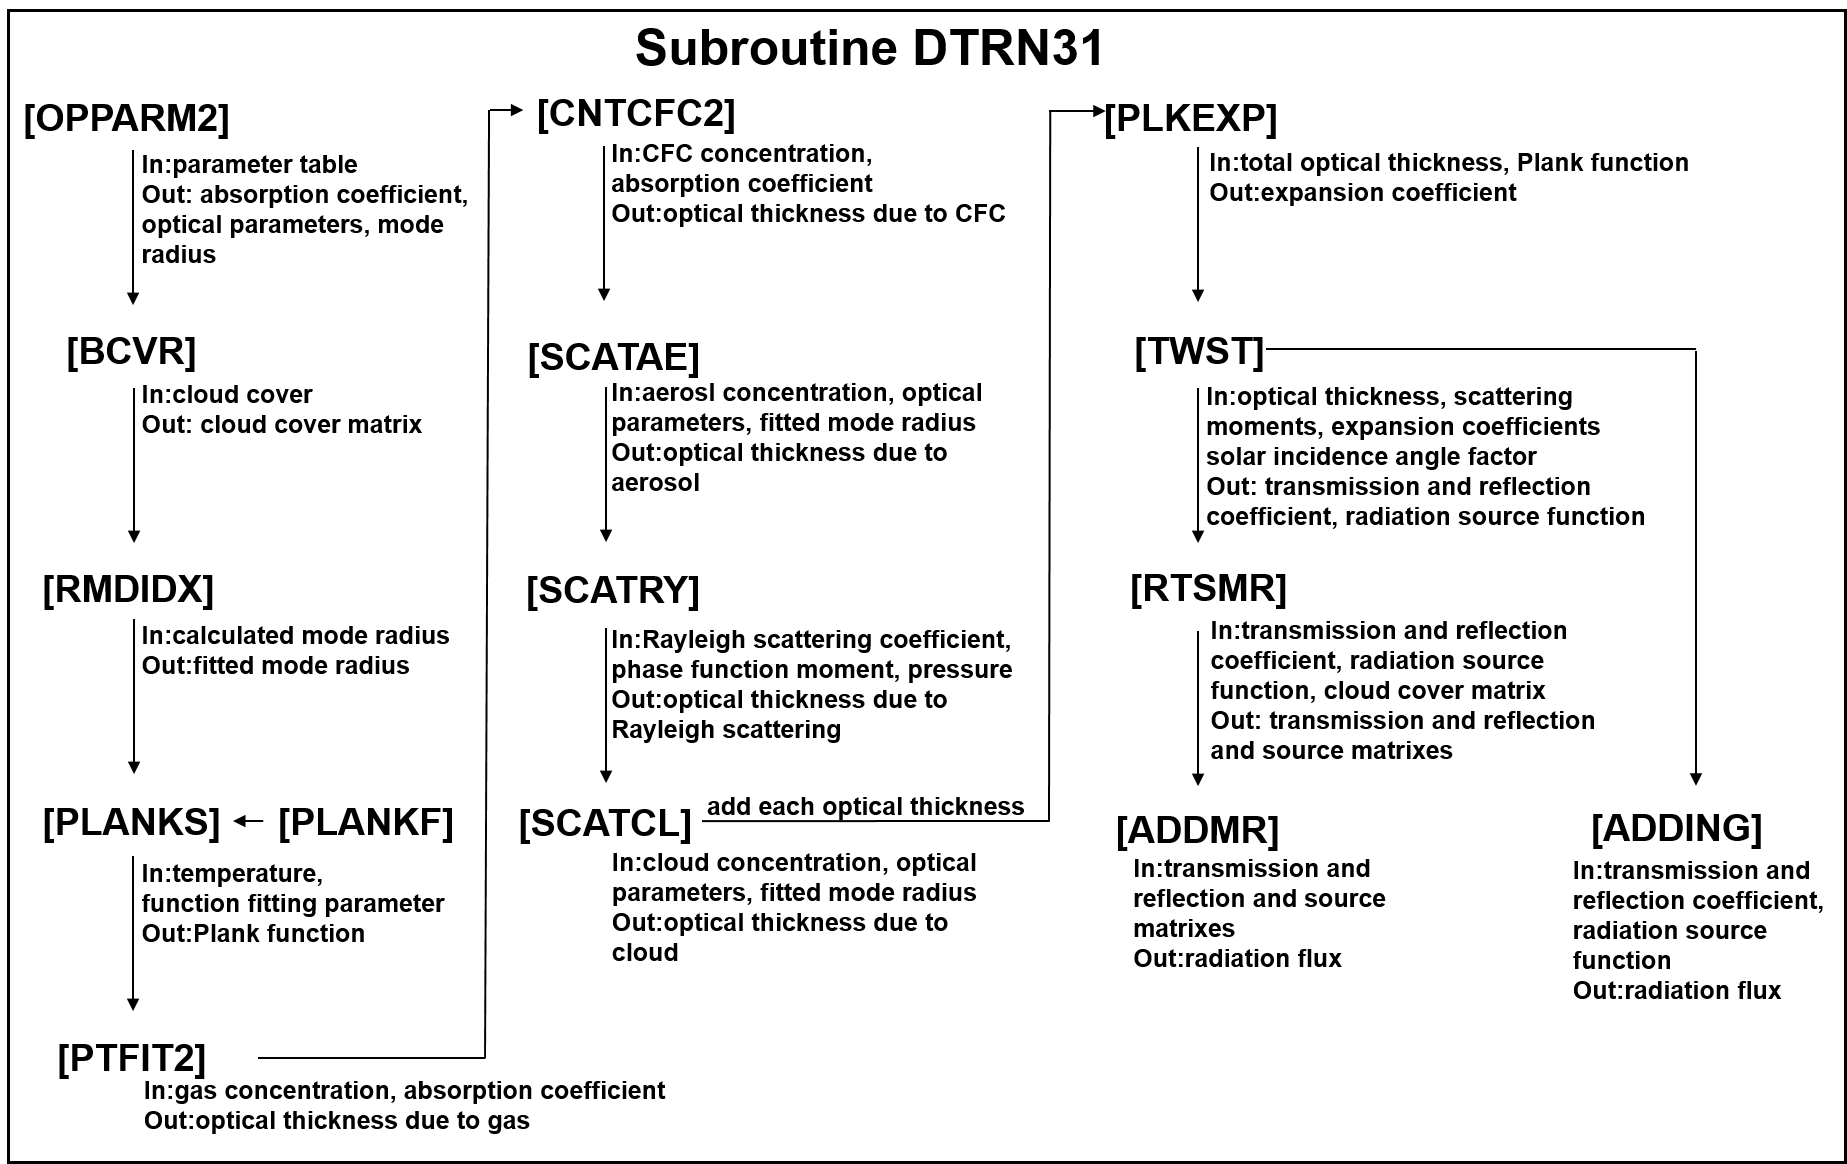
\includegraphics{Prad_Fig1.png}
\caption{Flowchart of \texttt{SUBROUTINE:{[}DTRN31{]}}}
\end{figure}

To account for the partial coverage of clouds, the transmission and
reflection coefficients and source functions for each layer are
calculated at weighted average of the cloud cover, separately for cloud
cover and clear-sky conditions. The cloud cover of the cumulus is also
considered. In addition, it also performs several adding and calculates
the clear-sky radiation flux.

\hypertarget{wavelength-and-sub-channel}{%
\subsubsection{Wavelength and
Sub-channel}\label{wavelength-and-sub-channel}}

The basics of radiative flux calculations are represented by
Beer-Lambert's Law.

\begin{eqnarray}
  F^\lambda(z) = F^\lambda(0) exp (-k^\lambda z)
\end{eqnarray}

\(F^{\lambda}\) is the radiant flux density at the wavelength of
\(\lambda\) and \(k^{\lambda}\) is the absorption coefficient. In order
to calculate the radiative fluxes related to the heating rate, the
integration operation with respect to the wavelength is required.

\begin{eqnarray}
  F(z) = \int F^\lambda(z) d \lambda= \int F^\lambda(0) exp (-k^\lambda z) d \lambda\
\end{eqnarray}

However, it is not easy to calculate this integration precisely because
the absorption and emission of radiation by gas molecules have the
complicated wavelength dependence of the absorption line attributed to
the structure of the molecule. The k-distribution method is a method
designed to make the relatively precise calculation easier. Within a
certain wavelength range, considering the density function \(F(k)\) for
\(\lambda\) of the absorption coefficient of \(k\), the above formula is
approximated as follows, \begin{eqnarray}
 \int F^\lambda(0) exp (-k^\lambda z) d \lambda
 \simeq \int \bar{F}^k(0) exp (-k z) F(k) dk
\end{eqnarray} where \(\bar{F}^k(0)\) is the flux averaged over a wavelength having
the absorption coefficient in this wavelength \(k\) in \(z=0\).

If \(\bar{F}^k(0)\) and \(F(k)\) are a relatively smooth functions to
the \(k\), \begin{eqnarray}
 \int F^\lambda(0) exp (-k^\lambda z) d \lambda
 \simeq \sum \bar{F}^i(0) exp (-k^i z) F^i
\end{eqnarray} the formula, as such above, can be relatively precisely calculated by
the addition of a finite number (sub-channels) of exponential terms.
This method has furthermore the advantage easy to consider the
absorption and scattering at the same time.

In the MIROC 6.0, by changing the radiation parameter data, the
calculations can be performed at various wavelengths. In the standard
version, the wavelength range is divided into 29 parts. In addition,
each wavelength range is divided into 1 to 6 sub-channels (corresponding
to the \(i\) in the above formula). There are 111 channels in total. The
wavelength range is divided by the wavenumber ( \(\mathrm{cm}^{-1}\) ),
1, 250, 400, 530, 610, 670, 750, 820, 980, 1175, 1225, 1325, 1400, 2000,
2500, 3300, 3800, 4700, 5200, 6000, 10000, 12750, 13250, 14750, 23000,
30000, 33500, 36000, 43500, 50000. Additionally, a chemical version is
also with 37 bands and 126 channels for chemical transport model and the
boundary of the shortwave region is also changed to 54000
\(\mathrm{cm}^{-1}\).

\hypertarget{calculation-of-the-planck-function}{%
\subsubsection{Calculation of the Planck
function}\label{calculation-of-the-planck-function}}

In this section, \texttt{SUBROUTINE:{[}PLANKS,\ PLANKF{]}} in pradt.F is
described.

The Planck function \(\bar{B}^{w}(T)\), integrated in each wavelength
range, is evaluated by the following formula. \begin{equation}
\bar{B}^{w}(T)=\lambda^{-2}{Texp}\left\{\sum_{n=1}^{5} B_{n}^{w}\left(\bar{\lambda}^{w} T\right)^{-n}\right\}
\end{equation} where \(\bar{\lambda}^{w}\) is the averaged wavelength of the
wavelength range, \(B_{n}^{w}\) is the parameter determined by function
fitting. This is calculated to the atmospheric temperature of each layer
\(T_l\), and the boundary atmospheric temperature of each layer
\(T_{l+1/2}\), surface temperature \(T_g\) and temperature
\(1\mathrm{K}\) higher than surface temperature \(T_{g+1K}\). The
calculations are performed for each wavelength and each layer. In the
following description, the subscript of the wavelength range \(w\) is
omitted.

\hypertarget{calculation-of-the-optical-thickness-to-gas-absorption}{%
\subsubsection{Calculation of the optical thickness to gas
absorption}\label{calculation-of-the-optical-thickness-to-gas-absorption}}

In this section, \texttt{SUBROUTINE:{[}PTFIT2{]}} in pradt.F is
described.

The optical thickness of the gas absorption (the line and continuum
absorption are unified) \(\tau^{K D}\) is expressed as follows by using
the index \(m\) as the type of molecules. \begin{equation}
\tau^{KD}=\sum_{m=1} k^{(m)} C^{(m)}
\end{equation} where \(k^{(m)}\) is the absorption coefficient of the molecule
\(m\), which is different for each sub-channel and determined as a
function of temperature \(T\) and atmospheric pressure \(p\).
\(C^{(m)}\) represents the amount of gas in the layer represented by
\(\mathrm{mol} / \mathrm{cm}^{2} / \mathrm{km}\), calculated by using
the gas concentration \(r^{(m)}\) in ppmv (
\(C^{(m)}=10^{-1} r^{(m)} \rho d z\) ). In the MIROC 6.0, the number of
the considered molecule types \(m\) is 6
(1:\(\mathrm{H}_{2} \mathrm{O}\), 2:\(\mathrm{C}\mathrm{O}_{2}\),
3:\(\mathrm{O}_{3}\), 4:\(\mathrm{N}_{2} \mathrm{O}\),
5:\(\mathrm{C}\mathrm{H}_{4}\), 6:\(\mathrm{O}_{2}\)). Also, \(k^{(m)}\)
is represented as follows (the details are in Sekiguchi and Nakajima,
2008). \begin{equation}
k^{(m)}=\exp \left(\log 10 k_{2}^{(m)}+(A+B T) \log \left(T / T_{\text {ref2 } }\right)\right)
\end{equation}

\begin{equation}
B=\left[\frac{\log 10\left(k_{3}^{(m)}-k_{2}^{(m)}\right)}{\log \left(\frac{T_{r e f 3}}{T_{r e f 2}}\right)}-\frac{\log 10\left(k_{1}^{(m)}-k_{2}^{(m)}\right)}{\log \left(\frac{T_{\text {ref1} }}{T_{\text {ref2}}}\right)}\right] /\left(T_{\text {ref3}}-T_{\text {ref1 }}\right)
\end{equation}

\begin{equation}
A=\frac{\log 10\left(k_{3}^{(m)}-k_{2}^{(m)}\right)}{\log \left(T_{\text {ref3 } } / T_{\text {ref2 } }\right)}-B T_{\text {ref3 }}
\end{equation}

\$ T\_ \{ref1-3\}\$ are the reference temperatures prepared in advance
(200, 260, 320 \(K\)), and \(k_{1-3}^{(m)}\) are the absorption
coefficients when the reference temperatures \$ T\_\{ref1-3\}\$ is used
(also fitted at 26 atmospheric pressure grids).

When considering the absorption of \(\mathrm{H}_{2} \mathrm{O}\), we
calculate the optical thickness of the self-broadening and add
\(\tau^{self}\). \begin{equation}
\tau^{K D\left(\mathrm{H}_{2} \mathrm{O}\right)}=\tau^{K D\left(\mathrm{H}_{2} \mathrm{O}\right)}+\tau^{\text {self }}
\end{equation}

\begin{equation}
\tau^{\text {self }}=\frac{k^{\left(\mathrm{H}_{2} \mathrm{O}_{-} \mathrm{self}\right)} C^{\left(\mathrm{H}_{2} \mathrm{O}\right)^{2}}}{C^{\left(\mathrm{H}_{2} \mathrm{O}\right)}+\rho d z 10^{5}}
\end{equation}

\(k^{(\mathrm{H}_{2} \mathrm{O}_{-} \mathrm{self})}\) is calculated in
the same way as \(k^{(m)}\). The self-broadening absorption coefficients
in the reference temperatures \(T_{ref1-3}\) are prescribed and
dependent on the pressure. In the above formula, \(10^{5}\) is
multiplied to convert the unit from \(\mathrm{km}\) to \(\mathrm{cm}\).
This calculation is done for each sub-channel and each layer.

\hypertarget{calculation-of-the-optical-thickness-to-cfc-absorption}{%
\subsubsection{Calculation of the optical thickness to CFC
absorption}\label{calculation-of-the-optical-thickness-to-cfc-absorption}}

In this section, \texttt{SUBROUTINE:{[}CNTCFC2{]}} in pradt.F is
described.

The optical thickness of the CFC absorption \(\tau^{CFC}\) is considered
for several types of CFCs \(m\). \begin{equation}
\tau^{C F C}=\sum_{m} 10^{k^{(m)}} r^{(m)} \rho \Delta z 10^{-1}
\end{equation} In MIROC 6.0, the number of the considered CFCs \(m\) is 28
(1:\(\mathrm{CFC\text{-11}}\), 2:\(\mathrm{CFC\text{-12}}\),
3:\(\mathrm{CFC\text{-13}}\), 4:\(\mathrm{CFC\text{-14}}\),
5:\(\mathrm{CFC\text{-113}}\), 6:\(\mathrm{CFC\text{-114}}\),
7:\(\mathrm{CFC\text{-115}}\), 8:\(\mathrm{HCFC\text{-21}}\),
9:\(\mathrm{HCFC\text{-22}}\), 10:\(\mathrm{HCFC\text{-123}}\),
11:\(\mathrm{HCFC\text{-124}}\), 12:\(\mathrm{HCFC\text{-141b}}\),
13:\(\mathrm{HCFC\text{-142b}}\), 14:\(\mathrm{HCFC\text{-225ca}}\),
15:\(\mathrm{HCFC\text{-225cb}}\), 16:\(\mathrm{HFC\text{-32}}\),
17:\(\mathrm{HFC\text{-125}}\), 18:\(\mathrm{HFC\text{-134}}\),
19:\(\mathrm{HFC\text{-134a}}\), 20:\(\mathrm{HFC\text{-143a}}\),
21:\(\mathrm{HFC\text{-152a}}\), 22:\(\mathrm{S}\mathrm{F}_{6}\),
23:\(\mathrm{ClON}\mathrm{O}_{2}\), 24:\(\mathrm{C}\mathrm{Cl}_{4}\),
25:\(\mathrm{N}_{2}\mathrm{O}_{5}\),
26:\(\mathrm{C}_{2}\mathrm{F}_{6}\), 27:\(\mathrm{HN}\mathrm{O}_{4}\),
28:\(\mathrm{SF}_{5}\mathrm{CF}_{3}\)). In the above formula,
\(10^{-1}\) is multiplied to convert from \(\mathrm{km}\) to
\(\mathrm{cm}\), and from ppmv to ratio. This calculation is done for
each sub-channel and each layer. This calculation is performed for each
layer and the wavelength range from about 540 to 1800
\(\mathrm{cm}^{-1}\).

\hypertarget{optical-thickness-to-scattering-and-scattering-moment}{%
\subsubsection{Optical thickness to scattering and scattering
moment}\label{optical-thickness-to-scattering-and-scattering-moment}}

Calculate the optical thickness of scattering and the scattering moment.
These calculations are performed for each wavelength and each layer. The
optical parameters for the particle matter \(q_{m}^{(p)}\) are prepared,
including the extinction coefficient (\(m = 1\)) including the
scattering and absorption process and the absorption coefficient
(\(m = 2\)) the moments of the volume scattering phase function
(\(m=3\text{-}4\): first-second order).

\hypertarget{aerosol}{%
\paragraph{Aerosol}\label{aerosol}}

In this section, \texttt{SUBROUTINE:{[}SCATAE{]}} in pradt.F is
described.

The optical thickness \(\tau^{a e}\), the part of the optical thickness
due to absorption \(\tau_{ab}^{a e}\), the scattering moment
\(Q_{m}^{a e}\) for aerosol are \begin{equation}
\tau^{a e}=\sum_{p} q_{1, n}^{(p)} r^{(p)} \times \rho \Delta z 10^{-1}
\end{equation}

\begin{equation}
\tau_{ab}^{a e}=\sum_{p} q_{2, n}^{(p)} r^{(p)} \times \rho \Delta z 10^{-1}
\end{equation}

\begin{equation}
Q_{m}^{a e}=\sum_{p} q_{m, n}^{(p)} r^{(p)} \times \rho \Delta z 10^{-1} (\mathrm{~m} \geq 3)
\end{equation}

\(p\) is the aerosol type, and \(r^{(p)}\) is volume mixing ratio of the
particle. The optical parameters for the particle \(q_{m, n}^{(p)}\)
depend on the mode radius index \(n\) prescribed for each particle
(IRA). In the MIROC 6.0, the number of the considered aerosol types
\(p\) 15 (1-6:soil dust (bin1-6), 7:carbonaceous (BC/OC=0.3),
8:carbonaceous (BC/OC=0.15), 9:carbonaceous (BC/OC=0), 10:black carbon
(external mixture), 11:sulfate, 12-15:sea salt (bin 1-4)).

If the aerosol radius is used, the optical thickness \(\tau^{a e}\), the
part of the optical thickness due to absorption \(\tau_{ab}^{a e}\), and
the scattering moment \(Q_{m}^{a e}\) for the hygroscopic aerosols
(e.g., carbonaceous, sulfate, sea salt) are \begin{equation}
\tau^{a e}=\sum_{p}\left[\left(1-F X_{a e}\right) q_{1, n f i t}^{(p)} r^{(p)}+F X_{a e} q_{1, n f i t+1}^{(p)} r^{(p)}\right] \times \rho \Delta z 10^{-1}
\end{equation}

\begin{equation}
\tau_{ab}^{a e}=\sum_{p}\left[\left(1-F X_{a e}\right) q_{2, n f i t}^{(p)} r^{(p)}+F X_{a e} q_{2, n f i t+1}^{(p)} r^{(p)}\right] \times \rho \Delta z 10^{-1}
\end{equation}

\begin{equation}
Q_{m}^{a e}=\sum_{p}\left[\left(1-F X_{a e}\right) q_{m, n f i t}^{(p)} r^{(p)}+F X_{a e} q_{m, n f i t+1}^{(p)} r^{(p)}\right] \times \rho \Delta z 10^{-1}(\mathrm{~m} \geq 2)
\end{equation}

\begin{equation}
F X_{a e}=\left(R H-R H_{n f i t}^{(r e f)}\right)\left(\frac{1}{R H_{n f i t+1}^{(r e f)}-R H_{n f i t}^{(r e f)}}\right)
\end{equation}

where \(RH\) is the local relative humidity and
\(R H_{n f i t}^{(r e f)}\) is the relative humidity given in the
parameter and \(nfit\) is the number of the prescribed relative humidity
closest to the \(RH\). \(nfit\) and \(FX_{ae}\) are calculated in the
\texttt{SUBROUTINE:{[}RMDIDX{]}} in pradt.F and determined in advance.
In the above formulas, \(10^{-1}\) is multiplied to convert from
\(\mathrm{km}\) to \(\mathrm{cm}\), and from ppmv to ratio.

\hypertarget{rayleigh-scattering-scatry}{%
\paragraph{\texorpdfstring{Rayleigh scattering
\texttt{{[}SCATRY{]}}}{Rayleigh scattering {[}SCATRY{]}}}\label{rayleigh-scattering-scatry}}

In this section, \texttt{SUBROUTINE:{[}SCATRY{]}} in pradt.F is
described.

The optical thickness \(\tau^{r}\) of Rayleigh scattering and the part
of the optical thickness due to absorption \(\tau_{ab}^{r}\) are

\begin{equation}
\tau^{r}=\frac{e^{r} d p q m o l_{1}}{p_{S T D}}
\end{equation}

\begin{equation}
\tau_{ab}^{r}=\frac{e^{r} d p q m o l_{2}}{p_{S T D}}
\end{equation}

\begin{equation}
p_{S T D}=1013.25
\end{equation}

where \(e^{r}\) is the Rayleigh scattering coefficient, \(qmol_m\) is
the moments of the phase function. These calculations are performed up
to \(m=2\). Also, this is added to the optical thickness for the
aerosol. \begin{equation}
\tau^{a e+r}=\tau^{a e}+\tau^{r}
\end{equation}

\begin{equation}
\tau_{ab}^{a e+r}=\tau_{ab}^{a e}+\tau_{ab}^{r}
\end{equation}

\hypertarget{cloud}{%
\paragraph{Cloud}\label{cloud}}

In this section, \texttt{SUBROUTINE:{[}SCATCL{]}} in pradt.F is
described.

The optical thickness \(\tau^{cl}\), the part of the optical thickness
due to absorption \(\tau_{ab}^{cl}\), and the scattering moment
\(Q_{m}^{c l}\) for cloud are \begin{equation}
\tau^{c l}=\sum_{c t} q_{1, n}^{(c t)}r^{(c t)}\times \rho \Delta z 10^{-1}
\end{equation}

\begin{equation}
\tau_{ab}^{c l}=\sum_{c t} q_{2, n}^{(c t)}r^{(c t)}\times \rho \Delta z 10^{-1}
\end{equation}

\begin{equation}
Q_{m}^{c l}=\sum_{c t} q_{m, n}^{(c t)} \times r^{(c t)} \rho \Delta z 10^{-1}(\mathrm{~m} \geq 3)
\end{equation}

\(ct\) is the cloud particle type (1:liquid cloud, 2:ice cloud). The
optical parameters for the particle \(q_{m, n}^{(c t)}\) depend on the
mode radius index \(n\) prescribed for each particle (IRC). If the cloud
radius is used, the optical thickness \(\tau^{cl}\), the part of the
optical thickness due to absorption \(\tau_{ab}^{cl}\), and the
scattering moment \(Q_{m}^{c l}\) for cloud are \begin{equation}
\tau^{c l}=\sum_{c t}\left[\left(1-F X_{c l}\right) q_{1, n f i t}^{(c t)} r^{(c t)}+F X_{c l} q_{1, n f i t+1}^{(c t)} r^{(c t)}\right] \times \rho \Delta z 10^{-1}
\end{equation}

\begin{equation}
\tau_{ab}^{c l}=\sum_{c t}\left[\left(1-F X_{c l}\right) q_{2, n f i t}^{(c t)} r^{(c t)}+F X_{c l} q_{2, n f i t+1}^{(c t)} r^{(c t)}\right] \times \rho \Delta z 10^{-1}
\end{equation}

\begin{equation}
Q_{m}^{c l}=\sum_{c t}\left[\left(1-F X_{c l}\right) q_{m, n f i t}^{(c t)} r^{(c t)}+F X_{c l} q_{m, n f i t+1}^{(c t)} r^{(c t)}\right] \times \rho \Delta z 10^{-1}(\mathrm{~m} \geq 3)
\end{equation}

\begin{equation}
F X_{c l}=\left(R^{(c t)}-R_{n f i t}^{(r e f)}\right)\left(\frac{1}{R_{n f i t+1}^{(r e f)}-R_{n f i t}^{(r e f)}}\right)
\end{equation}

where \(R^{(ct)}\) is the calculated mode radius and
\(R_{n f i t}^{(r e f)}\) is the mode radius given in the parameter and
\(nfit\) is the number of the prescribed mode radius closest to the
\(R^{(ct)}\). \(nfit\) and \(FX_{cl}\) are calculated in the subroutine
\texttt{SUBROUTINE:{[}RMDIDX{]}} in pradt.F and determined in advance.
In the above formulas, \(10^{-1}\) is multiplied to convert from
\(\mathrm{km}\) to \(\mathrm{cm}\), and from ppmv to ratio.

Finally, the total optical thickness for particle scattering, Rayleigh
scattering and absorption \(\tau^p\) and the contribution of scattering
\(\tau^{scat}\) are obtained as follows. \begin{equation}
\tau^{P}=\tau^{c l}+\tau^{a e+r}
\end{equation}

\begin{equation}
\tau^{s c a t}=\tau^{P}-\left(T_{ab}^{c l}+T_{ab}^{a e+r}\right)
\end{equation}

In addition, the moments of the normalized phase function \(G\) are
calculated up to the three orders. The zeroth moment \(G_1\) is trivial
from the normalization condition of the phase function. The first and
second moments \(G_2\), \(G_3\), are referred as the asymmetry factor
\(g\) and the truncation factor \(f\). \begin{equation}
G_{1}=1.0
\end{equation}

\begin{equation}
G_{m-1}=\frac{Q_{m}^{c l}+Q_{m}^{ae}}{\tau^{s c a t}}(m \geq 3), \quad G_{2}=g, \quad G_{3}=f
\end{equation}

This calculation is divided into the cloudy, clear sky and cumulus
conditions. In the cloudy and cumulus conditions, \(\tau^{cl}\) in the
0.5 and 0.67 \(\mathrm{{\mu}m}\) regions is as recorded as
\(\tau^{vis}\) in subroutine DTRN31.

**\(R^{ct}\) is calculated in \texttt{SUBROUTINE:RADFLX} as follows. \begin{equation}
R^{(c t)}=\left(\frac{3}{4 \pi} \frac{\rho r^{(c t)}}{\rho_{w}^{(c t)} n_{c}^{(c t)}}\right)^{1 / 3}
\end{equation} \(\rho_{w}^{(c t)}\) is the liquid or ice density. \(r^{ct}\) is the
amount of the liquid or ice cloud and calculated as follows. \begin{equation}
r^{(c t)}=\frac{C_{s t} r_{s t}^{(c t)}+C_{c u} r_{c u}^{(c t)}}{1-\left(1-C_{s t}\right)\left(1-C_{c u}\right)}
\end{equation} \(C\) is the area of the cloud, and the subscript \(st\) and \(cu\)
mean the stratus and cumulus. When \(r_{s t, c u}^{(c t)}\) is the small
amount in the stratosphere, it is reset to 0. \(n_{c}^{(c t)}\) is the
number density of cloud particles. \begin{equation}
n_{c}^{(l i q)}=\max \left(\frac{q_{a e}^{l i q} p N_{A}}{R T_{v}\left(18 \times 10^{-3} R_{v} / R\right)}, f_{l i q} n_{\min }^{(l i q)}\right)
\end{equation}

\begin{equation}
n_{c}^{(i c e)}=\max \left(\frac{q_{a e}^{i c e} p N_{A}}{R T_{v}\left(18 \times 10^{-3} R_{v} R_{v} / R\right)},\left(1-f_{l i q}\right) n_{\min }^{(i c e)}\right)
\end{equation}

where \(q_{a e}^{l i q}\) is the mixing ratio of the aerosol particles
calculated by the SPRINTERS and converted to the number concentration,
and \(n_{\min }^{(c t)}\) is the minimum number of the cloud particles.
and \(f_{liq}\) is liquid fraction. Also, \(n_{c}^{(c t)}\) is
calculated as follows when using OPT\_AECL\_SIMPLE. \begin{equation}
n_{c}^{(c t)}=\frac{\varepsilon n_{a} n_{m a x}^{(c t)}}{\varepsilon n_{a}+n_{\max }^{(c t)}}
\end{equation} where \(n_a\) is the number density of aerosol particles give as an
external condition, and \(\varepsilon\) and \(n_{\max }^{(c t)}\) are
constants. \(f_{liq}\) is calculated by the following formula using the
amount of cloud water \(w\) (\(0 \leq f_{\text {liq }} \leq 1\)). \begin{equation}
f_{l i q}=\frac{w_{s t} f_{l i q, s t}+w_{c u} f_{l i q, c u}}{w_{s t}+w_{c u}}
\end{equation}

\hypertarget{total-optical-thickness-dtrn31}{%
\subsubsection{\texorpdfstring{Total optical thickness
\texttt{{[}DTRN31{]}}}{Total optical thickness {[}DTRN31{]}}}\label{total-optical-thickness-dtrn31}}

All optical thickness including gaseous band absorption, and scattering
is, \begin{equation}
\tau=\tau^{K D}+\tau^{C O N}+\tau^{P}
\end{equation} where because \(\tau^{K D}\) is different for each subchannel, the
calculation is done for each sub-channel and each layer, and divided
into the cloudy, clear sky, and cumulus conditions.

\hypertarget{expansion-of-the-plank-function}{%
\subsubsection{Expansion of the plank
function}\label{expansion-of-the-plank-function}}

In this section, \texttt{SUBROUTINE:{[}PLKEXP{]}} in pradt.F is
described.

In each layer, the Planck function \(B\) is expanded as follows and the
expansion coefficients \(b_0\), \(b_1\), and \(b_2\), are obtained. \begin{equation}
{B}\left(\tau^{\prime}\right)=b_{0}+b_{1} \tau^{\prime}+b_{2}\left(\tau^{\prime}\right)^{2}
\end{equation} Here, as \({B}\left(\tau^{\prime}\right)\), \(B\) at the top of each
layer (the boundary with the top layer) is used, and as \({B}(\tau)\),
\(B\) at the bottom edge of each layer (the boundary with the layer
below), and as \({B}(\tau / 2)\), the \(B\) at the representative level
of each layer. \begin{equation}
b_{0}=B(0)
\end{equation}

\begin{equation}
b_{1}=(4{~B}(\tau / 2)-{B}(\tau)-3{~B}(0)) / \tau
\end{equation}

\begin{equation}
b_{2}=2({~B}(\tau)-{B}(0)-2{~B}(\tau / 2)) / \tau^{2}
\end{equation}

\begin{figure}
\centering
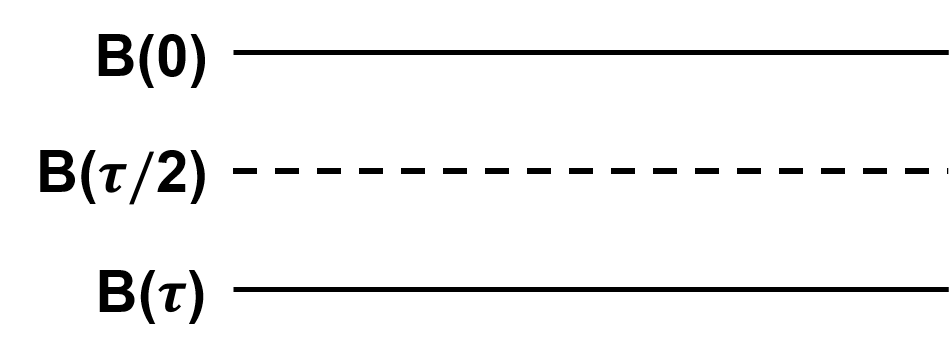
\includegraphics{Prad_Fig2.png}
\caption{Second-order expansion using the optical thickness of the plank
function}
\end{figure}

This calculation is done for each sub-channel and each layer and divided
into the cloudy, clear sky and cumulus conditions.

\hypertarget{transmission-and-reflection-coefficients-and-source-function}{%
\subsubsection{Transmission and reflection coefficients, and source
function}\label{transmission-and-reflection-coefficients-and-source-function}}

In this section, \texttt{SUBROUTINE:{[}TWST{]}} in pradt.F is described.

Using the obtained optical thickness \(\tau\), optical thickness of
scattering \(\tau^{scat}\), scattering moments \(g\), \(f\), expansion
coefficients for Planck function \(b_n\), and solar incidence angle
factor \(\mu_{0}\), the transmission coefficient \(T\), reflection
coefficient \(R\), downward radiation source function \(\epsilon^{+}\),
and the upward radiation source function \(\epsilon^{-}\) are founded,
by assuming a uniform layer and using the two-stream approximation.

The single-scattering albedo \(\omega\) is, \begin{equation}
\omega=\tau^{\text{scat}}/\tau
\end{equation} The optical thickness \(\tau^{*}\), the single-scattering albedo
\(\omega^{*}\), and asymmetric factor \(g^{*}\), corrected by the
contribution from the forward scattering factor \(f\) are, \begin{equation}
\tau^{*}=\tau(1-\omega f)
\end{equation}

\begin{equation}
\omega^{*}=\frac{(1-f) \omega}{1-\omega f}
\end{equation}

\begin{equation}
g^{*}=\frac{g-f}{1-f}
\end{equation}

\(\mu\) is a two-stream directional cosine. \begin{equation}
\mu \equiv\left(\frac{1}{\sqrt{3}}, \frac{1}{1.66}\right) \text { (shortwave, longwave) }
\end{equation}

\begin{equation}
W^{-} \equiv \mu^{-1 / 2}
\end{equation}

Furthermore, \begin{equation}
\hat{P}^{\pm}=\omega^{*} W^{-2}\left(1 \pm 3 g^{*} \mu^{2}\right) / 2
\end{equation}

\begin{equation}
\hat{S}_{s}^{\pm}=\omega^{*} W^{-}\left(1 \pm 3 g^{*} \mu_{0} \mu\right)
\end{equation}

can be determined as above as a normalized scattering phase function. \begin{equation}
\begin{aligned}
X &=\mu^{-1}-\left(\hat{P}^{+}-\hat{P}^{+}\right) \\
&=\mu^{-1}-3 \omega^{*} W^{-2} \mu^{2} g^{*} \\
\end{aligned}
\end{equation} \begin{equation}
\begin{aligned}
Y &=\mu^{-1}-\left(\hat{P}^{+}+\hat{P}^{+}\right) \\
&=\mu^{-1}-\omega^{*} W^{-2} \\
\end{aligned}
\end{equation}

\begin{equation}
\begin{aligned}
\hat{\sigma}_{S}^{+} &=\hat{S}_{S}^{+}+\hat{S}_{S}^{-} \\
&=\omega^{*} W^{-} \\
\end{aligned}
\end{equation}

\begin{equation}
\begin{aligned}
\hat{\sigma}_{S}^{-} &=\hat{S}_{s}^{+}-\hat{S}_{S}^{-} \\
&=3 \omega^{*} \mu_{0} W^{-} \mu g^{*}
\end{aligned}
\end{equation}

Using the above formula, the reflectance \(R\) and transmission \(T\)
become \begin{equation}
\begin{array}{c}
A A=\frac{X\left(1+e^{-\lambda \tau^{*}}\right)-\lambda\left(1-e^{-\lambda \tau^{*}}\right)}{X\left(1+e^{-\lambda \tau^{*}}\right)+\lambda\left(1-e^{-\lambda \tau^{*}}\right)} \\
\end{array}
\end{equation} \begin{equation}
\begin{array}{c}
B B=\frac{X\left(1-e^{-\lambda \tau^{*}}\right)-\lambda\left(1+e^{-\lambda \tau^{*}}\right)}{X\left(1-e^{-\lambda \tau^{*}}\right)+\lambda\left(1+e^{-\lambda \tau^{*}}\right)} \\
\end{array}
\end{equation}

\begin{equation}
\begin{array}{c}
\lambda=\sqrt{X Y} \\
\end{array}
\end{equation}

\begin{equation}
\begin{array}{c}
R=\frac{1}{2}(A A+B B) \\
\end{array}
\end{equation}

\begin{equation}
\begin{array}{c}
T=\frac{1}{2}(A A-B B)
\end{array}
\end{equation}

Next, we find the source function derived from the Planck function. \begin{equation}
\hat{b}_{n}=2 \pi\left(1-\omega^{*}\right) W^{-}\left(\frac{1}{1-\omega f}\right)^{n} b_{n}
\end{equation} The expansion coefficients of the radiation source function can be
found from the above formulas. \begin{equation}
\begin{array}{l}
D_{2}^{\pm}=\frac{\hat{b}_{2}}{Y} \\
\end{array}
\end{equation} \begin{equation}
\begin{array}{l}
D_{1}^{\pm}=\frac{\hat{b}_{1}}{Y} \mp \frac{2 \hat{b}_{2}}{X Y} \\
\end{array}
\end{equation}

\begin{equation}
\begin{array}{l}
D_{0}^{\pm}=\frac{\hat{b}_{0}}{Y}+\frac{2 \hat{b}_{2}}{X Y^{2}} \mp \frac{\hat{b}_{1}}{X Y} \\
\end{array}
\end{equation}

\begin{equation}
\begin{array}{l}
D^{\pm}\left(\tau^{*}\right)=D_{0}^{+}+D_{1}^{+} \tau^{*}+D_{2}^{+} \tau^{* 2}
\end{array}
\end{equation}

The radiation source function derived from the Planck function
\(\hat{\epsilon}_{A}^{\pm}\) is \begin{equation}
\begin{array}{l}
\hat{\epsilon}_{A}^{-}=D_{0}^{-}-R D_{0}^{-}-T D^{-}\left(\tau^{*}\right) \\
\end{array}
\end{equation} \begin{equation}
\begin{array}{l}
\hat{\epsilon}_{A}^{+}=D^{+}\left(\tau^{*}\right)-T D_{0}^{+}-R D^{-}\left(\tau^{*}\right)
\end{array}
\end{equation}

On the other hand, the radiation source function of the solar-induced
radiation is \begin{equation}
\begin{array}{l}
\hat{\epsilon}_{S}^{+}=F_{\text {sol }}\left(V_{s}^{+} e^{-\frac{\tau^{*}}{\mu_{0}}}-T V_{s}^{+}-R V_{s}^{-} e^{-\frac{\tau^{*}}{\mu_{0}}}\right)
\end{array}
\end{equation} \begin{equation}
\begin{array}{l}
\hat{\epsilon}_{S}^{+}=F_{\text {sol }}\left(V_{s}^{+} e^{-\frac{\tau^{*}}{\mu_{0}}}-T V_{s}^{+}-R V_{s}^{-} e^{-\frac{\tau^{*}}{\mu_{0}}}\right)
\end{array}
\end{equation}

Here, \(Q \gamma\) and \(V_{s}^{\pm}\) are expressed by the following
formulas, and \(F_{sol}\) is solar irradiance. \begin{equation}
\begin{array}{c}
V_{s}^{\pm}=\frac{1}{2}\left[Q \gamma \pm\left(\frac{Q \gamma}{\mu_{0}}+\frac{\hat{\sigma}_{S}^{-}}{X}\right)\right] \\
\end{array}
\end{equation} \begin{equation}
\begin{array}{c}
Q \gamma=\frac{X \hat{\sigma}_{S}^{+} \mu_{0}+\mu_{0}^{-1} \hat{\sigma}_{S}^{-}}{X Y \mu_{0}+\mu_{0}^{-1}}
\end{array}
\end{equation}

The direct solar transmission is also calculated in this subroutine. \begin{equation}
E x^{d i r}=e^{-\tau^{*}/ \mu_{0}}
\end{equation} This calculation is done for each sub-channel and each layer and
divided into the cloudy, clear sky, and cumulus conditions.

\hypertarget{t-r-s-matrixes-for-maximalrandom-approximation}{%
\subsubsection{T, R, S matrixes for maximal/random
approximation}\label{t-r-s-matrixes-for-maximalrandom-approximation}}

In this section, \texttt{SUBROUTINE:{[}RTSMR{]}} in pradt.F is
described.

In this subroutine, T, R, S matrixes for maximal/random approximation is
made. The radiation source function, which is the sum of both the plank
function and the solar incident origins, is \begin{equation}
\begin{array}{l}
\epsilon^{-(\text {cloud})}=\hat{\epsilon}_{S}^{-(\text {cloud})} {Tr}^{(\text {cloud})}+\hat{\epsilon}_{A}^{-(\text {cloud})} C \\
\end{array}
\end{equation} \begin{equation}
\begin{array}{l}
\epsilon^{-(\text {clear})}=\hat{\epsilon}_{S}^{-(\text {clear})}{Tr}^{(\text {clear})}+\hat{\epsilon}_{A}^{-(\text {clear})}(1-C) \\
\end{array}
\end{equation}

\begin{equation}
\begin{array}{l}
\epsilon^{+(\text {cloud})}=\hat{\epsilon}_{S}^{+(\text {cloud})}{Tr}^{(\text {cloud})}+\hat{\epsilon}_{A}^{-(\text {cloud})} C \\
\end{array}
\end{equation}

\begin{equation}
\begin{array}{l}
\epsilon^{+(\text {clear})}=\hat{\epsilon}_{S}^{+(\text {clear})}{Tr}^{(\text {clear})}+\hat{\epsilon}_{A}^{-(\text {clear})}(1-C)
\end{array}
\end{equation}

\(Tr\) is the direct solar transmission for maximal/random approximation
and calculated as follows in \texttt{SUBROUTINE:DTRN31}. \begin{equation}
\begin{aligned}
\operatorname{Tr}_{n}^{(\text {cloud})} &=E x_{n}^{(\text {cloud})} B_{n}^{(3)}+E x_{n}^{(\text {clear})}\left(1-B_{n}^{(1)}\right) \\
\end{aligned}
\end{equation} \begin{equation}
\begin{aligned}
E x_{n+1}^{(\text {cloud})} &={Tr}_{n}^{(\text {cloud})} E x_{n}^{\operatorname{dir}(\text {cloud})} \\
\end{aligned}
\end{equation}

\begin{equation}
\begin{aligned}
T r_{n}^{(\text {clear})} &=E x_{n}^{(\text {cloud})}\left(1-B_{n}^{(3)}\right)+E x_{n}^{(\text {clear})} B_{n}^{(1)} \\
\end{aligned}
\end{equation}

\begin{equation}
\begin{aligned}
E x_{n+1}^{(\text {clear)} }&={Tr}_{n}^{(\text {clear})} E x_{n}^{\text {dir}(\text {clear})}
\end{aligned}
\end{equation}

\(Ex\) is the cumulative direct solar transmission. \(B_{n}^{(1-4)}\) is
the cloud cover interaction index and calculated in
\texttt{SUBROUTINE:{[}BCVR{]}}in pradt.F . \begin{equation}
\begin{array}{l}
B_{n}^{(1)}=\frac{1-\max \left(C_{n-1}, C_{n}\right)}{1-C_{n-1}} \\
\end{array}
\end{equation} \begin{equation}
\begin{array}{l}
B_{n}^{(2)}=\frac{1-\max \left(C_{n+1}, C_{n}\right)}{1-C_{n+1}} \\
\end{array}
\end{equation}

\begin{equation}
\begin{array}{l}
B_{n}^{(3)}=\frac{\min \left(C_{n-1}, C_{n}\right)}{C_{n-1}} \\
\end{array}
\end{equation}

\begin{equation}
\begin{array}{l}
B_{n}^{(4)}=\frac{\min \left(C_{n+1}, C_{n}\right)}{C_{n+1}}
\end{array}
\end{equation}

Next, T matrixes for maximal/random approximation are calculated. \begin{equation}
\begin{array}{l}
T^{+(cloud, 1)}=T^{(\text {cloud})} B^{(3)} \\
\end{array}
\end{equation}

\begin{equation}
\begin{array}{l}
T^{+(\text {cloud}, 2)}=T^{(\text {cloud})}\left(1-B^{(1)}\right)\\
\end{array}
\end{equation}

\begin{equation}
\begin{array}{l}
T^{+(\text {clear}, 1)}=T^{(\text {clear})}\left(1-B^{(3)}\right)\\
\end{array}
\end{equation}

\begin{equation}
\begin{array}{l}
T^{+(\text {clear}, 2)}=T^{(\text {clear})} B^{(1)} \\
\end{array}
\end{equation}

\begin{equation}
\begin{array}{l}
T^{-(\text {cloud}, 1)}=T^{(\text {cloud})} B^{(4)} \\
\end{array}
\end{equation}

\begin{equation}
\begin{array}{l}
T^{-(\text {cloud}, 2)}=T^{(\text {cloud})}\left(1-B^{(2)}\right)\\
\end{array}
\end{equation}

\begin{equation}
\begin{array}{l}
T^{-(\text {clear}, 1)}=T^{(\text {clear})}\left(1-B^{(4)}\right)\\
\end{array}
\end{equation}

\begin{equation}
\begin{array}{l}
T^{-(\text {clear}, 2)}=T^{(\text {clear})} B^{(2)}
\end{array}
\end{equation}

Also, R matrixes for maximal/random approximation are calculated. \begin{equation}
\begin{array}{l}
R^{+(\text {cloud}, 1)}=R^{(\text {cloud})} B^{(3)} \\
\end{array}
\end{equation} \begin{equation}
\begin{array}{l}
R^{+(\text {cloud}, 2)}=R^{(\text {cloud})}\left(1-B^{(1)}\right) \\
\end{array}
\end{equation}

\begin{equation}
\begin{array}{l}
R^{+(\text {clear}, 1)}=R^{(\text {clear})}\left(1-B^{(3)}\right) \\
\end{array}
\end{equation}

\begin{equation}
\begin{array}{l}
R^{+(\text {clear}, 2)}=R^{(\text {clear})} B^{(1)} \\
\end{array}
\end{equation}

\begin{equation}
\begin{array}{l}
R^{-(\text {cloud}, 1)}=R^{(\text {cloud})} B^{(4)} \\
\end{array}
\end{equation}

\begin{equation}
\begin{array}{l}
R^{-(\text {cloud,2})}=R^{(\text {cloud})}\left(1-B^{(2)}\right) \\
\end{array}
\end{equation}

\begin{equation}
\begin{array}{l}
R^{-(\text {clear}, 1)}=R^{(\text {clear})}\left(1-B^{(4)}\right) \\
\end{array}
\end{equation}

\begin{equation}
\begin{array}{l}
R^{-(\text {clear}, 2)}=R^{(\text {clear})} B^{(2)}
\end{array}
\end{equation}

This calculation is done for each sub-channel and each layer.

\hypertarget{adding-of-source-functions-for-each-layer}{%
\subsubsection{Adding of source functions for each
layer}\label{adding-of-source-functions-for-each-layer}}

In this section, \texttt{SUBROUTINE:{[}ADDMR\ or\ ADDING} in pradt.F is
described.

By using transmission coefficient \(T\), reflection coefficient \(R\),
and radiation source function \(\varepsilon\) in all layers, the
radiation fluxes \(u\) at each layer boundary can be obtained by using
the adding method. This means that the when two layers of \(T\), \(R\),
\(\varepsilon\) are known, the \(T\), \(R\), \(\varepsilon\) of the
whole combined layer of the two layers can be easily calculated.

\begin{figure}
\centering
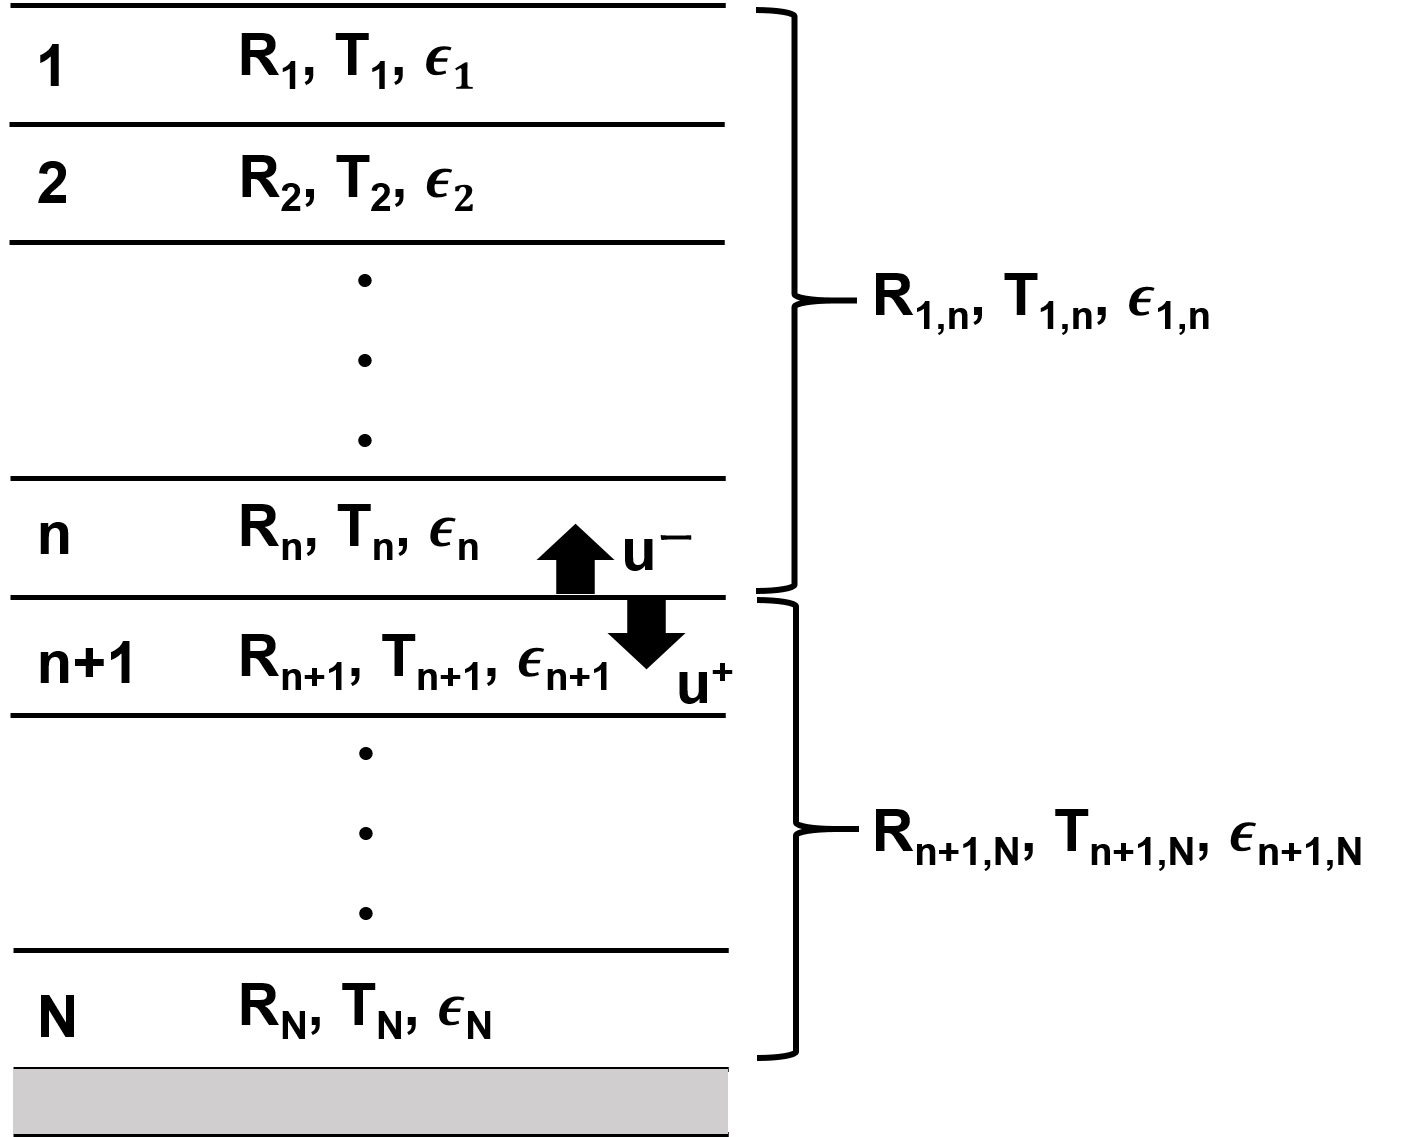
\includegraphics{Prad_Fig3.png}
\caption{Schematic illustration of the adding method}
\end{figure}

\hypertarget{subroutineaddmr}{%
\paragraph{\texorpdfstring{\texttt{SUBROUTINE:{[}ADDMR{]}}}{SUBROUTINE:{[}ADDMR{]}}}\label{subroutineaddmr}}

In this subroutine, the maximal/random flux in cloudy conditions is
calculated by the adding method and the T, R, and S matrixes are used
for calculations.

First, the upward radiation source function the bottom layer is
calculated.

In the shortwave region, \begin{equation}
\begin{array}{l}
\epsilon_{N}^{-(\text {cloud})}=W^{+} \alpha_{s} \mu_{0}\left(\frac{1}{\mu}\right) F_{0} e_{N}^{-\left\langle\tau^{*}\right\rangle / \mu_{0}(\text{cloud})} \\
\end{array}
\end{equation} \begin{equation}
\begin{array}{l}
\epsilon_{N}^{-(\text {clear})}=W^{+} \alpha_{s} \mu_{0}\left(\frac{1}{\mu}\right) F_{0} e_{N}^{-\left\langle\tau^{*}\right\rangle / \mu_{0} \text {(clear) }}
\end{array}
\end{equation}

\(\left\langle\tau^{*}\right\rangle\) indicates the total optical
thickness \(\tau^{*}\) of from the upper end of the atmosphere to the
upper end of the layer currently being considered and
\(e^{-\left\langle\tau^{*}\right\rangle / \mu_{0}}\) is calculated in
\texttt{SUBROUTINE:{[}ADDMR{]}} of pradt.F.

In the longwave region, \begin{equation}
\begin{array}{l}
\epsilon_{N}^{-(\text {cloud})}=\epsilon_{N}^{-(\text {cloud})}+W^{+} 2 \pi\left(1-\alpha_{s}\right) B_{N} C_{N} \\
\end{array}
\end{equation} \begin{equation}
\begin{array}{l}
\epsilon_{N}^{-(\text {clear})}=\epsilon_{N}^{-(\text {clear})}+W^{+} 2 \pi\left(1-\alpha_{s}\right) B_{N}\left(1-C_{N}\right)
\end{array}
\end{equation}

Here, \begin{equation}
W^{+} \equiv \mu^{1 / 2}
\end{equation} The reflectance \(R_{1, n}^{-}\) and source function
\(\epsilon_{1, n}^{+}\) regarded from the first to the \(n\) layers as a
single layer are \begin{equation}
\begin{array}{l}
\epsilon_{1, n}^{+}=\epsilon_{n}^{+}+T_{n}^{+}\left(1-R_{n}^{+} R_{1, n-1}^{-}\right)^{-1}\left(R_{1, n-1}^{-} \epsilon_{n}^{-}+\epsilon_{1, n-1}^{+}\right) \\
\end{array}
\end{equation} \begin{equation}
\begin{array}{l}
R_{1, n}^{-}=R_{n}^{-}+T_{n}^{+}\left(1-R_{n}^{+} R_{1, n-1}^{-}\right)^{-1} R_{1, n-1}^{-} T_{n}^{-}
\end{array}
\end{equation}

The upward and downward fluxes at the bottom of the atmosphere are \begin{equation}
\begin{array}{l}
u_{N+1 / 2}^{+}=\left(1-R_{1, N-1}^{-} R_{N}^{+}\right)^{-1}\left(\epsilon_{1, N-1}^{+}+R_{1, N-1}^{-} \epsilon_{N}^{-}\right) \\
\end{array}
\end{equation}

\begin{equation}
\begin{array}{l}
u_{N+1 / 2}^{-}=\left(1-R_{N}^{+} R_{1, N-1}^{-}\right)^{-1}\left(\epsilon_{N}^{-}+R_{N}^{+} \epsilon_{1, N-1}^{+}\right)
\end{array}
\end{equation}

Also, upward and downward fluxes at the boundary between layers \(n\)
and \(n+1\) are \begin{equation}
\begin{array}{l}
u_{n+1 / 2}^{+}=\left(1-R_{1, n-1}^{-} R_{n}^{+}\right)^{-1}\left(R_{1, n-1}^{-} T_{n}^{-} u_{n+1 / 2}^{-}+R_{1, n-1}^{-} \epsilon_{n}^{-}+\epsilon_{1, n}^{+}\right) \\
\end{array}
\end{equation} \begin{equation}
\begin{array}{l}
u_{n+1 / 2}^{-}=\left(1-R_{n}^{+} R_{1, n-1}^{-}\right)^{-1}\left(T_{n}^{-} u_{n+1 / 2}^{-}+R_{n}^{+} \epsilon_{1, n-1}^{+}+\epsilon_{n}^{-}\right)
\end{array}
\end{equation}

However, the upward and downward flux at the upper end of the atmosphere
is as follows. \begin{equation}
\begin{array}{l}
u_{1 / 2}^{+}=0 \\
\end{array}
\end{equation} \begin{equation}
\begin{array}{l}
u_{1 / 2}^{-}=T_{1}^{-} u_{1+1 / 2}^{-}+\epsilon_{1}^{-}
\end{array}
\end{equation}

Finally, since this flux is scaled, we rescaled and added the direct
solar incidence to the find the radiation flux. Furthermore, the flux in
the cloudy area and the clear sky area is added. \begin{equation}
\begin{array}{c}
F_{n+1 / 2}^{+}=\frac{W^{+}}{W}\left(u_{n+1 / 2}^{+(\text{cloud})}+u_{n+1 / 2}^{+(\text{clear})}\right)+\mu_{0} F_{0}\left(e_{n+1 / 2}^{-\left\langle\tau^{*}\right\rangle / \mu_{0}(\text {cloud})}\right) \\
\end{array}
\end{equation} \begin{equation}
\begin{array}{c}
F_{n+1 / 2}^{-}=\frac{W^{+}}{W}\left(u_{n+1 / 2}^{-(\text{cloud})}+u_{n+1 / 2}^{-(\text {clear})}\right)
\end{array}
\end{equation}

Also, surface direct downward radiation flux \(F_{s f}^{+}\) is \begin{equation}
F_{s f}^{+}=\mu_{0} F_{0}\left(e_{N}^{-\left\langle\tau^{*}\right\rangle / \mu_{0}(\text {cloud})}+e_{N}^{-\left\langle\tau^{*}\right\rangle / \mu_{0} \text{(clear)}}\right)
\end{equation} This calculation is done for each sub-channel.

\hypertarget{subroutineadding}{%
\paragraph{\texorpdfstring{\texttt{SUBROUTINE:{[}ADDING{]}}}{SUBROUTINE:{[}ADDING{]}}}\label{subroutineadding}}

Since the maximal/random approximation cannot be used under the clear
sky condition, this subroutine is used to calculate the flux.

First, the radiation source function, which is the sum of both the plank
function origin and the solar incident origin, is \begin{equation}
\epsilon^{\pm}=\hat{\epsilon}_{S}^{\pm} e^{-\left\langle\tau^{*}\right\rangle / \mu_{0}}+\hat{\epsilon}_{A}^{\pm}
\end{equation} There are layers \(1, 2,\dots, N\) from the top. The surface layer is
considered to be a single layer and the \(N\) layer. Given the
reflectance and source function of the layers from the n to the \(N\)
layer as a single layer \(R_{n, N}\), \(\epsilon_{n, N}^{-}\), \begin{equation}
\begin{array}{c}
R_{n, N}=R_{n, N}+T_{n}\left(1-R_{n+1, N} R_{n}\right)^{-1} R_{n+1} T_{n} \\
\end{array}
\end{equation} \begin{equation}
\begin{array}{c}
\epsilon_{n, N}^{-}=\epsilon_{n}^{-}+T_{n}\left(1-R_{n+1, N} R_{n}\right)^{-1}\left(R_{n+1, N} \epsilon_{n}^{+}+\epsilon_{n, N}^{-}\right)
\end{array}
\end{equation}

\begin{equation}
\begin{array}{c}
R_{n, N}=R_{n, N}+T_{n}\left(1-R_{n+1, N} R_{n}\right)^{-1} R_{n+1} T_{n} \\
\end{array}
\end{equation}

\begin{equation}
\begin{array}{c}
\epsilon_{n, N}^{-}=\epsilon_{n}^{-}+T_{n}\left(1-R_{n+1, N} R_{n}\right)^{-1}\left(R_{n+1, N} \epsilon_{n}^{+}+\epsilon_{n, N}^{-}\right)
\end{array}
\end{equation}

This can be solved by \(n=N-1,\dots,1\) in sequence, starting from the
values at the surface \(R_{N, N}\), \(\epsilon_{N, N}^{-}\). \begin{equation}
\begin{array}{c}
R_{N, N}=R_{N}=\alpha_{s} \\
\end{array}
\end{equation} \begin{equation}
\begin{array}{c}
\epsilon_{N, N}=W^{+}\left(\alpha_{s} \mu_{0}\left(\frac{1}{\mu}\right) e^{-\left\langle\tau^{*}\right\rangle / \mu_{0}} F_{0}+2 \pi\left(1-\alpha_{s}\right) B_{N}\right)
\end{array}
\end{equation}

The reflectance \(R_{1, n}\) and source function \(\epsilon_{1, n}^{+}\)
regarded from the first to the \(n\) layers as a single layer are \begin{equation}
\begin{array}{c}
R_{1, n}=R_{n}+T_{n}\left(1-R_{1, n-1} R_{n}\right)^{-1} R_{1, n-1} T_{n} \\
\end{array}
\end{equation} \begin{equation}
\begin{array}{c}
\epsilon_{1, N}^{+}=\epsilon_{n}^{+}+T_{n}\left(1-R_{1, n-1} R_{n}\right)^{-1}\left(R_{1, n-1} \epsilon_{n}^{-}+\epsilon_{1, n-1}^{+}\right)
\end{array}
\end{equation}

It can be solved by \(n=2,\dots, N\), starting from
\(R_{1,1}=R_{1}, \epsilon_{1,1}^{+}=\epsilon_{1}^{+}\).

With these, downward flux at the boundary between layers \(n\) and
\(n+1\), the downward and upward flux are came back to a problem between
two layers of combined layer, the combinations of layers \(1-n\) and
\(n+1-N\). \begin{equation}
\begin{array}{c}
u_{n+1 / 2}^{+}=\left(1-R_{1, n} R_{n+1, N}\right)^{-1}\left(\epsilon_{1, n}^{+}+R_{1, n} \epsilon_{n+1, N}^{-}\right) \\
\end{array}
\end{equation} \begin{equation}
\begin{array}{c}
u_{n+1 / 2}^{-}=R_{n+1, N} u_{n, n+1}^{+}+\epsilon_{n+1, N}^{-}
\end{array}
\end{equation}

can be written as above. However, the flux at the top of the atmosphere
is \begin{equation}
\begin{array}{c}
u_{1 / 2}^{+}=0 \\
\end{array}
\end{equation} \begin{equation}
\begin{array}{c}
u_{1 / 2}^{-}=\epsilon_{1, N}^{-}
\end{array}
\end{equation}

Finally, since this flux is scaled, we rescaled and added the direct
solar incidence to the find the radiation flux. \begin{equation}
\begin{array}{c}
F_{n+1 / 2}^{+}=\frac{W^{+}}{W} u_{n+1 / 2}^{+}+\mu_{0} e^{-\left\langle\tau^{*}\right\rangle / \mu_{0}} F_{0} \\
\end{array}
\end{equation} \begin{equation}
\begin{array}{c}
F_{n+1 / 2}^{-}=\frac{W^{+}}{W} u_{n+1 / 2}^{-}
\end{array}
\end{equation}

Also, surface direct downward radiation flux \(F_{s f}^{+}\) is \begin{equation}
F_{s f}^{+}=\mu_{0} F_{0} e^{-\left\langle\tau^{*}\rangle\ \mu_{0}\right.}
\end{equation}

\hypertarget{adding-in-the-flux}{%
\subsubsection{Adding in the flux}\label{adding-in-the-flux}}

\begin{equation}
F^{\pm}=\sum_{c} w_{c}\left(1-C_{c u}\right) \bar{F}^{\pm}+\sum_{c} w_{c} C_{c u} F^{c \pm}
\end{equation}

\begin{equation}
F^{\circ \pm}=\sum_{c} w_{c} F^{\circ \pm}
\end{equation}

If the radiation flux \(F_{C}^{\pm}\) is found for each sub-channel in
each layer, the wavelength-integrated flux is found by multiplying a
weight \(w_c\) correspondingly to a wavelength representative of the
sub-channel and adding. \(C_{cu}\) is the horizontal coverage of the
cumulus cloud. It is divided into the short wavelength range and long
wavelength range and added together. In addition, the downward flux of a
part of the short wavelength region (shorter than the wavelength of
0.7-0.8 \(\mathrm{{\mu}m}\)) at the surface is obtained as PAR
(photosynthetically active radiation). Also, the radiation flux in the
clear-sky condition is calculated (\(F^{\circ \pm}\)).

Also, in the shortwave region, we find the downward radiation at the
lower end of the atmosphere and the difference between the surface
direct downward radiation flux. \begin{equation}
F_{s f}^{+}=\sum_{c} w_{c}\left(1-C_{u}\right) \bar{F}_{N+1 / 2}^{+}+\sum_{c} w_{c} C_{c u} F_{N+1 / 2}^{c}
\end{equation}

\begin{equation}
F_{s f, d i f}^{+}=\sum_{c} w_{c}\left(1-C_{c u}\right)\left(\bar{F}_{N+1 / 2}^{+}-\bar{F}_{s f}^{+}\right)+\sum_{c} w_{c} C_{c u}\left(F_{N+1 / 2}^{c}-F_{s f}^{c}\right)
\end{equation}

This calculation is done in \texttt{SUBROUTINE:{[}DTRN31{]}}

\hypertarget{calculation-of-the-temperature-derivative-of-the-flux}{%
\subsubsection{Calculation of the temperature derivative of the
flux}\label{calculation-of-the-temperature-derivative-of-the-flux}}

To implicitly solve for surface temperature, calculate differential term
of upward flux with respect to surface temperature
\(\mathrm{d}F^{\mp}/dT_{g}\). Therefore, we obtained the value for
temperatures \(1\text{K}\) higher than \(T_g\)
\(\bar{B}^{w}\left(T_{g}+1\right)\) and used it to redo the flux
calculation using the addition method, and the difference from the
original value is set to \(\mathrm{d}F^{\mp}/dT_{g}\). This is a
meaningful value only in the longwave region (earth radiation region).
This calculation is done in \texttt{SUBROUTINE:{[}RADFLX{]}} of pradt.F.

\hypertarget{calculation-of-the-heating-rate}{%
\subsubsection{Calculation of the heating
rate}\label{calculation-of-the-heating-rate}}

The heating rate of the nth layer \(H_n\) is calculated by using the
radiation flux obtained so far. It is calculated separately for
shortwave and longwave ranges, and finally add together
(\texttt{SUBROUTINE:{[}RDTND{]}} in pradm.F). \begin{equation}
H_{n}=-\frac{\left(F_{n}^{-}-F_{n}^{-}\right)-\left(F_{n}^{+}-F_{n+1}^{+}\right)}{g C_{p} d p}
\end{equation}

\hypertarget{flux-of-incidence-and-incident-angle}{%
\subsubsection{Flux of incidence and incident
angle}\label{flux-of-incidence-and-incident-angle}}

In this section, \texttt{SUBROUTINE:{[}SHTINS{]}} in pradi.F is
described.

The following parameters are determined using the eccentricity \(e\),
with reference to Berger (1978). \begin{equation}
\begin{array}{l}
\beta=\sqrt{1-e^{2}} \\
\end{array}
\end{equation} \begin{equation}
\begin{array}{l}
a_{1}=-2\left(\frac{1}{2} e+\frac{1}{8} e^{3}\right)(1+\beta) \\
\end{array}
\end{equation}

\begin{equation}
\begin{array}{l}
a_{2}=-2\left(-\frac{1}{4} e^{2}\right)\left(\frac{1}{2}+\beta\right) \\
\end{array}
\end{equation}

\begin{equation}
\begin{array}{l}
a_{3}=-2\left(\frac{1}{8} e^{3}\right)\left(\frac{1}{2}+\beta\right) \\
\end{array}
\end{equation}

\begin{equation}
\begin{array}{l}
b_{1}=2 e-\frac{1}{4} e^{3} \\
\end{array}
\end{equation}

\begin{equation}
\begin{array}{l}
b_{2}=\frac{5}{4} e^{2} \\
\end{array}
\end{equation}

\begin{equation}
\begin{array}{l}
b_{3}=\frac{13}{12} e^{3}
\end{array}
\end{equation}

Additionally, \begin{equation}
\begin{array}{l}
\epsilon=\frac{e p s d}{180} \pi \\
\end{array}
\end{equation} \begin{equation}
\begin{array}{l}
\varpi=\frac{v p i d+180}{180} \pi
\end{array}
\end{equation}

where \(epsd\) and \(vpid\) are the angle of the obliquity and the
precession.

Earth position \(\lambda_{m}\) at a time \(t_m\) is represented by using
the position of the vernal equinox \(\lambda_{0}\). \begin{equation}
\begin{array}{c}
\lambda_{0}=a_{1} \sin (-\varpi)+a_{2} \sin (-2 \varpi)+a_{3} \sin (-3 \varpi) \\
\end{array}
\end{equation} \begin{equation}
\begin{array}{c}
\lambda_{m}=\frac{t_{m}-t_{0}}{2 \pi \times 365 \times 86400}+\lambda_{0}
\end{array}
\end{equation}

The solar declination \(\delta\) is \begin{equation}
\delta=\arcsin (\sin \epsilon \sin (V+\varpi))
\end{equation} \begin{equation}
\\V=\lambda_{m}-\varpi+b_{1} \sin \left(\lambda_{m}-\varpi\right)+b_{2} \sin 2\left(\lambda_{m}-\varpi\right)+b_{3} \sin 3\left(\lambda_{m}-\varpi\right)
\end{equation}

The incident angle \(\cos \zeta\) is founded by using the latitude
\(\varphi\), the solar declination \(\delta\), and the hour angle at a
point of longitude \(h\). \begin{equation}
\mu_{0}=\cos \zeta=\sin \varphi \sin \delta+\cos \varphi \cos \delta \cosh
\end{equation} Incident Flux \(F_0\) is represented as follows, \begin{equation}
\begin{array}{c}
F_{0}=F_{00} r^{-2} \\
\end{array}
\end{equation} \begin{equation}
\begin{array}{c}
r=\frac{1-e^{2}}{1+e(\cos V+\varpi)}
\end{array}
\end{equation}

where \(F_{00}\) is the solar constant and is the ratio of the ratio to
the time of the distance between the sun and the earth. The number of
times when \(\cos \zeta \geq 0\) (in the daytime) in time increments
(set in NHSUB), is counted, and \(F_{0}\) and \(\cos \zeta\) are finally
averaged.

It is also possible to give average annual insolation. In this case, the
annual and day mean incidence and angle of incidence are approximated as
follows. \begin{equation}
\begin{array}{c}
\bar{F}=F_{00} / \pi \\
\end{array}
\end{equation}

\begin{equation}
\begin{array}{c}
\bar{\mu}_{0} \simeq 0.410+0.590 \cos ^{2} \varphi
\end{array}
\end{equation}

\hypertarget{reading-the-each-parameter}{%
\subsubsection{Reading the each
parameter}\label{reading-the-each-parameter}}

In \texttt{SUBROUTINE:{[}OPPARM2{]}}of pradt.F, various parameters used
for radiation calculation are read. The outline of the procedure is
shown below.

\begin{enumerate}
\def\labelenumi{\arabic{enumi}.}
\item
  Read the numbers of bands, the radiances representative of upward and
  downward radiation, the grids of the pressure \(\log (\mathrm{p})\),
  grid of the temperatures, the optical flag, and CFCs.
\item
  Read the band boundaries and the information of the pressure grid and
  temperature grid.
\item
  First, the optical property flag, the number of channels, the weights
  for channels and the number of the molecules including in a waveband
  are read. The optical property flag is modified in order to
  distinguish the PAR, 0.67, 0.5, and 10.5 \(\mathrm{{\mu}m}\).
  Additionally, molecule ID and \(k\)-width are read for each molecule.
  Finally, the absorption coefficient for the self-broadening and CFC
  are also done only when the optical property flag in the band is
  positive. The k-width and the absorption coefficient for the
  self-broadening are arranged in the order of the grid of the
  temperatures, the grids of the pressures, and the channels. Step 3 is
  performed for each wavelength band.
\item
  First, the number of particles is read. Next, the numbers of the modes
  and the mode radius (or relative humidity) are read for each particle.
  Using the mode radius (or relative humidity), the following parameter
  required to interpolate the calculated values is calculated for each
  mode number. \begin{equation}
  \frac{1}{R_{n+1}^{(r e f)}-R_{n}^{(r e f)}}
  \end{equation}
\item
  Read the band boundaries again.
\item
  Read the Plank function coefficient, solar insolation, surface
  properties (not output), Rayleigh scattering coefficient, Rayleigh
  scattering phase function. The moment for particle scattering phase
  function is read in the order of the particle and the optical number
  and read up to the second moment. Step 6 is performed for each
  wavelength band.
\end{enumerate}

\hypertarget{other-notes}{%
\subsubsection{Other notes}\label{other-notes}}

The calculation of the radiation is usually not done at every step.
Thus, the radiation flux is saved, and it is used if the time is not
used for radiation calculation. As for the shortwave radiation, using
the percentage of time (time is \(\mu_{0}>0\)) between the next
calculation time \(f\) and the solar incidence angle factor averaged
over the daylight hours \(\bar{\mu}_{0}\), seek the Flux \(\bar{F}\), \begin{equation}
{F}=f \frac{\mu_{0}}{\bar{\mu}_{0}} \bar{F}
\end{equation}

% 物理過程:拡散フラックス
\hypertarget{vertical-diffusion.}{%
\subsection{Vertical Diffusion.}\label{vertical-diffusion.}}

\hypertarget{vertical-diffusion-scheme-overview.}{%
\subsubsection{Vertical Diffusion Scheme
Overview.}\label{vertical-diffusion-scheme-overview.}}

The vertical diffusion scheme, due to sub-grid scale turbulent
diffusion. Evaluating the vertical flux of physical quantities. The main
input data are wind speed, \(u, v\), \(u, v\), and temperature \(T\) The
specific humidity \(q\), the cloud cover \(l\), is The output data are
the vertical fluxes of momentum, heat, water vapor, cloud water and It
is the differential value for obtaining an implicit solution.

To estimate the vertical diffusion coefficient, the Mellor and Yamada
(1974, 1982). The turbulent closure model. Using level 2
parameterization.

The outline of the calculation procedure is as follows.

\begin{enumerate}
\def\labelenumi{\arabic{enumi}.}
\item
  as the stability of the atmosphere. Richardson numbers.
\item
  calculate the diffusion coefficient from Richardson number
  \texttt{MODULE:{[}VDFCOF{]}}.
\item
  calculate the flux and its derivative from the diffusion coefficient.
\end{enumerate}

\hypertarget{basic-formula-for-flux-calculations}{%
\subsubsection{Basic Formula for Flux
Calculations}\label{basic-formula-for-flux-calculations}}

The vertical diffuse flux in the atmosphere is , Using the diffusion
coefficient \(K\), it is evaluated as follows.

\begin{eqnarray}
  F{u} = K_{M} \frac{\partial u}{\partial \sigma} 
\end{eqnarray}

\begin{eqnarray}
  F{v} = K_M \frac{\partial v}{\partial \sigma} 
\end{eqnarray}

\begin{eqnarray}
  F{\theta} = K_H \frac{\partial \theta}{\partial \sigma} 
\end{eqnarray}

\begin{eqnarray}
  F{q} = K_q \frac{\partial q}{\partial \sigma} 
\end{eqnarray}

\hypertarget{richardson-number.}{%
\subsubsection{Richardson Number.}\label{richardson-number.}}

The standard for atmospheric stratospheric stability, Bulk Richardson
number \(R_{iB}\) is

\begin{eqnarray}
R_{iB} = \frac{\displaystyle 
               \frac{g}{\theta_s} \frac{\Delta \theta}{\Delta z} }
              {\displaystyle
                  \left( \frac{\Delta u}{\Delta z} \right)^2 
                + \left( \frac{\Delta v}{\Delta z} \right)^2      }
\end{eqnarray}

. defined by . Here, \((\Delta A)_{k-1/2}\) represents
\(A_{k} - A_{k-1}\). The \((\Delta z)_{k-1/2}\) is based on the
hydrostatic pressure equation,

\begin{eqnarray}
(\Delta z)_{k-1/2} = \frac{R Tv_{k}}{g} 
                     \frac{(\Delta \sigma)_{k-1/2}}{\sigma_{k-1/2}}
\end{eqnarray}

The flux Ricahrdson number \(R_{if}\) is ,

\begin{eqnarray}
R_{if} = \frac{1}{2 \beta_2}
      \left[ \beta_1 + \beta_4 R_{iB}
              - \sqrt{ ( \beta_1 + \beta_4 R_{iB} )^2 
                       - 4 \beta_2 \beta_3 R_{iB} }
              \right] ,
\end{eqnarray}

However,

\begin{eqnarray}
\alpha_1  =  3 A_2 \gamma_1  \\
\alpha_2  =  3 A_2 (\gamma_1+\gamma_2) \\
\beta_1   =  A_1 B_1 ( \gamma_1 - C_1 ) \\
\beta_2   =  A_1 [ B_1 ( \gamma_1 - C_1 ) + 6 A_1 + 3 A_2 ] \\
\beta_3   =  A_2 B_1 \gamma_1 \\
\beta_4   =  A_2 [ B_1 ( \gamma_1 + \gamma_2 ) - 3 A_1 ] ,
\end{eqnarray}

\begin{eqnarray}
(A_1, B_1, A_2, B_2, C_1 ) = ( 0.92, 16.6, 0.74, 10.1, 0.08 ) ,
\end{eqnarray}

\begin{eqnarray}
\gamma_1 = \frac{1}{3} - \frac{2 A_1}{B_1}\, , \, \, \, 
\gamma_2 = \frac{B_2}{B_1} + 6\frac{A_1}{B_1} .
\end{eqnarray}

The relationship between the \(R_{iB}\) and the \(R_{if}\) is
illustrated in this figure, Figure {[}p-dif:rib-rif{]}{]}
(\#p-dif:rib-rif).

\hypertarget{diffusion-coefficient.}{%
\subsubsection{Diffusion Coefficient.}\label{diffusion-coefficient.}}

The diffusion coefficient is , For each layer boundary (\(k-1/2\) level)
, It is given as follows.

\begin{eqnarray}
K_M        =  l^2 \frac{\Delta |\mathbf{v}|}{\Delta z} S_M  \\
K_H = K_q  =  l^2 \frac{\Delta |\mathbf{v}|}{\Delta z} S_H 
\end{eqnarray}

Here, \(S_M, S_H\) are,

\begin{eqnarray}
\widetilde{S_H} = \frac{ \alpha_1-\alpha_2 R_{if} }{ 1-R_{if} }
\end{eqnarray}

\begin{eqnarray}
\widetilde{S_M} = \frac{ \beta_1-\beta_2 R_{if} }{ \beta_3-\beta_4 R_{if} } 
                  \widetilde{S_H} ,
\end{eqnarray}

with ,

\begin{eqnarray}
S_M  =  B_1^{1/2} ( 1- R_{if} )^{1/2} 
          \widetilde{S_M}^{3/2} \\
S_H  =  B_1^{1/2} ( 1- R_{if} )^{1/2} 
          \widetilde{S_M}^{1/2} \widetilde{S_H} .
\end{eqnarray}

\(l\) is a mixing distance, according to Blakadar (1962),

\begin{eqnarray}
l = \frac{kz}{1+kz/l_0}
\end{eqnarray}

Take. \(k\) is a Kárman constant. The current standard value is
\(l_0=200\) m.

If \(S_H, S_M\) are shown as functions of \(R_{if}\),
Figure\protect\hyperlink{p-dif:smsh-rif}{p-dif:smsh-rif{]}} Yes.

\hypertarget{calculating-flux.}{%
\subsubsection{Calculating Flux.}\label{calculating-flux.}}

Using the above, we calculate the fluxes and flux derivatives.

\begin{eqnarray}
  Fu_{k-1/2} = K_{M,k-1/2}(u_{k-1}-u_{k})/(\sigma_{k-1}-\sigma_{k})
\end{eqnarray}

\begin{eqnarray}
  Fv_{k-1/2} = K_{M,k-1/2}(v_{k-1}-v_{k})/(\sigma_{k-1}-\sigma_{k})
\end{eqnarray}

\begin{eqnarray}
  F\theta_{k-1/2} 
  = K_{H,k-1/2}(\theta_{k-1}-\theta_{k})/(\sigma_{k-1}-\sigma_{k})
\end{eqnarray}

\begin{eqnarray}
  Fq_{k-1/2} = K_{q,k-1/2}(q_{k-1}-q_{k})/(\sigma_{k-1}-\sigma_{k})
\end{eqnarray}

\begin{eqnarray}
     \frac{\partial Fu_{k-1/2}}{\partial u_{k-1}} =   \frac{\partial Fv_{k-1/2}}{\partial v_{k-1}} 
  = -\frac{\partial Fu_{k-1/2}}{\partial u_{k}} = - \frac{\partial Fv_{k-1/2}}{\partial v_{k}}  
  = K_{M,k-1/2}/(\sigma_{k-1}-\sigma_{k})
\end{eqnarray}

\begin{eqnarray}
  \frac{\partial F\theta_{k-1/2}}{\partial T_{k-1}}
  = \sigma_{k-1}^{-\kappa} K_{H,k-1/2}/(\sigma_{k-1}-\sigma_{k})
\end{eqnarray}

\begin{eqnarray}
  \frac{\partial F\theta_{k-1/2}}{\partial T_{k}}
 = \sigma_{k}^{-\kappa} K_{H,k-1/2}/(\sigma_{k-1}-\sigma_{k})
\end{eqnarray}

\begin{eqnarray}
  \frac{\partial Fq_{k-1/2}}{\partial u_{k-1}}
 = - \frac{\partial Fq_{k-1/2}}{\partial u_{k}}
 = K_{q,k-1/2}/(\sigma_{k-1}-\sigma_{k})
\end{eqnarray}

\hypertarget{minimum-diffusion-coefficient.}{%
\subsubsection{Minimum Diffusion
Coefficient.}\label{minimum-diffusion-coefficient.}}

In the very stable case, the above estimate gives zero as the diffusion
coefficient. As it is, the model's behavior can be modified in various
ways Set a suitable minimum value as it will have a negative effect. The
current standard values are the same for all fluxes and \(K_{min}=\)
0.15 m\(^{2}\)/s

\hypertarget{other-notes.}{%
\subsubsection{Other Notes.}\label{other-notes.}}

I'm calling the shallow cumulus convection \texttt{MODULE:{[}SHLCOF{]}},
By default, this is a dummy.

% 物理過程:地表フラックス

\subsection{地表フラックス}

\subsubsection{地表フラックススキームの概要}

地表フラックススキームは, 
接地境界層における乱流輸送による
大気地表間の物理量のフラックスを評価する.
主な入力データは, 風速 TERM00000,TERM00000, 気温 TERM00001, 比湿 TERM00002 であり,
出力データは, 運動量, 熱, 水蒸気の鉛直フラックスと
implicit 解を得るための微分値である.

バルク係数は Louis(1979), Louis {\em et al.}(1982) に従って求める. 
ただし, 運動量と熱に対する粗度の違いを考慮した補正を行なっている. 

計算手順の概略は以下の通りである.
\begin{enumerate}
\item 大気の安定度として
      Richardson 数を計算する.
\item Richardson 数からバルク係数を計算する \texttt{MODULE:[PSFCL]}.
\item バルク係数からフラックスとその微分を計算する.
\item 必要であれば, 求められたフラックスを用いて
      海面の粗度効果・自由対流の効果・風速補正を考慮した後に,
      もう一度計算を行なう.
\end{enumerate}

\subsubsection{フラックス計算の基本式}

地表フラックス TERM00003,TERM00003 は
バルク係数 TERM00004,TERM00004 を用いて
次のように表される.
%
\begin{quote}
EQ=00000.
\end{quote}
\begin{quote}
EQ=00001.
\end{quote}
\begin{quote}
EQ=00002.
\end{quote}
\begin{quote}
EQ=00003.
\end{quote}
%
ただし, TERM00005 は可能蒸発量である.
実蒸発量の計算は「地表過程」ならび
「大気地表系の拡散型収支式の解法」の節で述べる.

\subsubsection{Richardson 数}

大気地表間の安定度の基準となる,
バルクRichardson数 TERM00006 は
%
\begin{quote}
EQ=00004.
\end{quote}
ここで, 
\begin{quote}
EQ=00005.
\end{quote}
は補正ファクターで, 補正前のバルク Richardson数から近似的に求めるが, 
ここでは計算方法は略す. 

\subsubsection{バルク係数}

バルク係数 TERM00007,TERM00007 は
Louis(1979), Louis {\em et al.}(1982) に従って求める. 
ただし, 運動量と熱に対する粗度の違いを考慮した補正を行なっている. 
すなわち, 運動量, 熱, 水蒸気に対する粗度を
それぞれ TERM00008,TERM00008 とすると
一般に TERM00009,TERM00009 であるが, 熱, 水蒸気についても
TERM00010 の高さからのフラックスに対するバルク係数
TERM00011, TERM00012 をまず求め, その後に補正する. 
%
\begin{quote}
EQ=00006.
\end{quote}
%
\begin{quote}
EQ=00007.
\end{quote}
\begin{quote}
EQ=00008.
\end{quote}
%
\begin{quote}
EQ=00009.
\end{quote}
\begin{quote}
EQ=00010.
\end{quote}

TERM00013,TERM00013 は
中立時の(TERM00014 からのフラックスに対する)バルク係数で,
%
\begin{quote}
EQ=00011.
\end{quote}

補正ファクター TERM00015 は, 
\begin{quote}
EQ=00012.
\end{quote}
であるが, 計算方法は略す. 
係数は, TERM00016,TERM00016 である. 

バルク係数の TERM00017 依存性を図示すると,
図\ref{p-sflx:cm}, 図\ref{p-sflx:ch}のようになる.

\begin{figure}[htbp]
  \begin{center}
    \epsfile{file=sflx-cm.ps,width=70mm}
    \caption{運動量に対する粗度}
    \label{p-sflx:cm}
  \end{center}
\end{figure}
\begin{figure}[htbp]
  \begin{center}
    \epsfile{file=sflx-ch.ps,width=70mm}
    \caption{熱に対する粗度. TERM00018 の場合}
    \label{p-sflx:ch}
  \end{center}
\end{figure}

\subsubsection{フラックスの計算}

これにより, フラックスが計算される.
%
\begin{quote}
EQ=00013.
\end{quote}
\begin{quote}
EQ=00014.
\end{quote}
\begin{quote}
EQ=00015.
\end{quote}
\begin{quote}
EQ=00016.
\end{quote}

微分項は, 以下のようになる.
\begin{quote}
EQ=00017.
\end{quote}
\begin{quote}
EQ=00018.
\end{quote}
\begin{quote}
EQ=00019.
\end{quote}
\begin{quote}
EQ=00020.
\end{quote}
\begin{quote}
EQ=00021.
\end{quote}

ここで, 注意したいのは,
TERM00019 はこの時点では求められていない量であることである.
表皮温度は, 
地表熱バランスの条件
\begin{quote}
EQ=00022.
\end{quote}
を満たすように決まる.
この時点では, TERM00020 としては前の時間ステップにおけるものを使って評価する.
地表バランスを満たす本当のフラックスの値は,
地表過程と結合してこの式を解いてから定まる.
その意味で, 上のフラックスに TERM00021 をつけておいた.

\subsubsection{海面における取扱い}

海面では, Miller et al.(1992) に従い, 以下の2つの効果を考慮している.
\begin{itemize}
\item 風速が弱いときに自由対流運動が卓越すること
\item 海面の粗度が風速によって変化すること
\end{itemize}

自由対流運動の効果は, 浮力フラックス TERM00022 を計算し,
\begin{quote}
EQ=00023.
\end{quote}
TERM00023 のときに,
\begin{quote}
EQ=00024.
\end{quote}
\begin{quote}
EQ=00025.
\end{quote}
とすることで考慮する.  TERM00024 は混合層の厚さのスケールに対応する.
現在の標準値は TERM00025 m である.
% この自由対流運動の効果は, 海面以外でも考慮している.

海面の粗度変化は, 摩擦速度 TERM00026
\begin{quote}
EQ=00026.
\end{quote}
を用いて,
\begin{quote}
EQ=00027.\\
EQ=00027.\\
EQ=00027.
\end{quote}
のように評価する. TERM00027 TERM00028 TERM00029 は
大気の動粘性係数であり, 
他の係数の標準値は
TERM00030,TERM00030,
TERM00031,TERM00031,
TERM00032,TERM00032 である.

以上の計算では, TERM00033,TERM00033 が必要であるため,
逐次近似計算を行なう.

\subsubsection{風速の補正}

一般に粗度の大きな地表では, 粗度の小さな地表に比べて
運動量の下向き輸送が効率的であるためにその直上の風が弱く,
粗度による TERM00034 の違いを風速の違いによって打ち消す効果が働く.

モデルにおいて地表フラックス計算に渡される風速は
力学過程の時間積分によって計算された値であり,
スペクトル展開によって平滑化された値となっている.
そのために, 海面と陸面など, 粗度の大きく違う地表が
小さなスケールで混在している領域では, 
この補償効果がうまく表現できない.
そのため, 一度運動量フラックスを計算し,
大気最下層の風速をそれによって補正してから
もういちど運動量・熱・水のフラックスを計算しなおす.

\subsubsection{風速の最小値}

小規模運動の効果を考え,
地表フラックスの算出の際の地表風速
TERM00035 の最小値を設定する.
現在の標準値は, 各フラックスに共通で
3m/s である.


% 物理過程:地表モデル
\hypertarget{surface-flux-scheme-sea-surface}{%
\subsection{Surface Flux Scheme (Sea
Surface)}\label{surface-flux-scheme-sea-surface}}

Until
\href{https://github.com/MIROC-DOC/model_description/blob/master/org/AGCM5.6-Tech.pdf}{CCSR/NIES
AGCM (1997)}, both land surface and sea surface were treated as one of
the atmospheric physical processes, but after MIROC3
(\href{https://ccsr.aori.u-tokyo.ac.jp/~hasumi/miroc_description.pdf}{Hasumi
and Emori, 2004}), land surface processes became independent as MATSIRO.
However, since MIROC3
(\href{https://ccsr.aori.u-tokyo.ac.jp/~hasumi/miroc_description.pdf}{Hasumi
and Emori, 2004}), land surface processes have been separated into
MATSIRO
(\href{https://www.sciencedirect.com/science/article/pii/S0921818103000304}{Takata
et al., 2003};
\href{https://journals.ametsoc.org/doi/pdf/10.1175/JCLI-D-13-00310.1}{Nitta
et al., 2014}). In \texttt{SUBROUTINE:{[}SURFCE{]}} in pgsfc.F,
\texttt{ENTRY:{[}OCNFLX{]}} (in \texttt{SUBROUTINE:{[}OCEAN{]}} of
pgocn.F) is called for the sea surface, and \texttt{ENTRY:{[}LNDFLX{]}}
(in \texttt{SUBROUTINE:{[}MATSIRO{]}} of matdrv.F) is called for the
land surface, respectively. This chapter describes sea surface
processes, which are still treated within the framework of atmospheric
physical processes in MIROC6
(\href{https://www.geosci-model-dev.net/12/2727/2019/gmd-12-2727-2019.pdf}{Tatebe
et al., 2019})). For the land surface processes, please refer to
\href{https://github.com/integrated-land-simulator/model_description}{Description
of ILS}.

Sea surface processes provide the boundary conditions at the lower end
of the atmosphere through the exchange of momentum, heat, and water
fluxes between the atmosphere and the surface. In
\texttt{ENTRY:{[}OCNFLX{]}}, the following procedure is used to deal
with sea surface processes.

\begin{enumerate}
\def\labelenumi{\arabic{enumi}.}
\tightlist
\item
  prepare variables for sea ice extent and no ice extent, respectively,
  using sea ice concentration.
\item
  Determine the surface boundary conditions.
\item
  Calculate the flux balance.
\item
  Calculate the radiation budget at the sea surface.
\item
  Calculate the deposition by CHASER.
\item
  solve the heat balance at the sea surface and update the skin
  temperature and each flux value.
\end{enumerate}

No prognostic variables are used in this scheme.

Practically, precipitation flux from 2 schemes are treated together.

\begin{eqnarray}
    Pr = Pr_c + Pr_l
\end{eqnarray}

where \(Pr\) is total precipitation flux, \(Pr_c\) is precipitation flux
from the cumulus convection scheme, and \(Pr_l\) is precipitation flux
from the large scale condensation scheme, respectively.

Sea ice covered/free areas are represented by \(L=1,2\). Each area is
calculated then weighted by sea ice concentration (\(R_{ice}\)).

In the sea ice area (\(L=1\)), the skin temperature (\(T_s\)) is the sea
ice skin temperature (\(T_{ice}\)). However, if \(T_{ice}\) is higher
than the melting point (\(T_{melt}=273.15 \mathrm{[K]}\)), then
\(T_{melt}\) is used.

\begin{eqnarray}
    T_s = min(T_{ice},T_{melt})
\end{eqnarray}

The sea ice bottom temperature (\(T_b\)) is assumed to be the sea skin
temperature (\(T_{o(1)}\)).

\begin{eqnarray}
    T_b = T_{o(1)}
\end{eqnarray}

The amount of sea ice (\(W_{ice}\)) and the amount of snow on it
(\(W_{snow}\)) are converted per unit area by considering sea ice
concentration (\(R_{ice}\)) and used in the calculation. However, a
limiter (\(\epsilon\)) is provided to prevent the values from becoming
too small.

\begin{eqnarray}
R_{ice} =\mathrm{max}( R_{ice,orginal}, \epsilon)
\end{eqnarray}

In the ice-free area (\(L=2\)), the skin temperature (\(T_s\)) and sea
ice bottom temperature (\(T_b\)) are assumed to be the sea temperature
temperature (\(T_{o(1)}\)).

\begin{eqnarray}
    T_s = T_b = T_{o(1)}
\end{eqnarray}

The evaporation efficiency is set to 1 for both \(L=1, 2\).

If sea ice concentration (\(R_{ice}\)) is not given (as a boundary
condition or from an OGCM), it is simply diagnosed with the sea ice
volume (\(W_{ice}\)) in \texttt{ENTRY:{[}OCNICR{]}} (in
\texttt{SUBROUTINE:{[}OCNICR{]}} of pgocn.F).

\begin{eqnarray}
R_{ice} = \mathrm{min}\Big(\sqrt{\frac{\mathrm{max}(W_{ice},0)}{W_{ice,c}}},1.0\Big)
\end{eqnarray}

The standard gives the amount of sea ice per area as
\(W_{ice,c}=300 \mathrm{[kg/m^2]}\).

\hypertarget{boundary-conditions-ocnbcs}{%
\subsubsection{\texorpdfstring{Boundary Conditions
\texttt{{[}OCNBCS{]}}}{Boundary Conditions {[}OCNBCS{]}}}\label{boundary-conditions-ocnbcs}}

In \texttt{ENTRY{[}OCNBCS{]}} (in \texttt{SUBROUTINE:{[}OCNSUB{]}} of
pgocn.F), surface albedo and roughness are calculated. They are
calculated supposing ice-free conditions, then modified.

First, let us consider the sea surface level albedo
(\(\alpha_{(d,b)}\)), \(b=1,2,3\) represent the visible, near-infrared,
and infrared wavelength bands, respectively. Also, \(d=1,2\) represents
direct and scattered light, respectively. The albedo for the visible
bands are calculated in \texttt{SUBROUTINE\ {[}SEAALB{]}} (of pgocn.F),
supposing ice-free conditions. The albedo for near-infrared is set to
same as the visible one. The albedo for infrared is uniformly set to a
constant value.

The grid-averaged albedo, taking into account sea ice concentration
(\(R_{ice}\)), is

\begin{eqnarray}
    \alpha = \alpha -R_{ice} \alpha_{ice}
\end{eqnarray}

\(\alpha_{ice}\) is given as
\(\alpha_{ice,1}=0.5,\alpha_{ice,2}=0.5,\alpha_{ice,3}=0.05\),
respectively.

In addition, we want to consider the effect of snow cover. Here, we
consider the albedo modification by temperature. Standard threshold
values for snow temperature are \(T_{al,2}=258.15 \mathrm{[K]}\) and
\(T_{al,1}=273.15 \mathrm{[K]}\). The snow albedo changes linearly with
temperature change from \(\alpha_{snow,1}=0.75\) to
\(\alpha_{ snow,2}\). Let the coefficient \(\tau_{snow}\), which is
\(0\le \tau \le 1\).

\begin{eqnarray}
\tau_{snow} = \frac{T_s - T_{al,1}}{T_{al,2}-T_{al,1}}
\end{eqnarray}

Update the snow albedo (\(\alpha_{snow}\)) as

\begin{eqnarray}
    \alpha_{snow} = \alpha_{snow,0} + \tau_{snow}(\alpha_{snow,2}-\alpha_{snow,1})
\end{eqnarray}

Second, let us consider sea surface roughnesses. Roughnesses of for
momentum, heat and vapor are calculated in
\texttt{SUBROUTINE:{[}SEAZ0F{]}} (of pgocn.F), supposing the ice-free
conditions.

When the sea ice exists (\(L=1\)), roughnesses of momentum, heat and
vapor (\(r_{0,M},r_{0,H},r_{0,E}\)) is modified to take into account sea
ice concentration (\(R_{ice}\)),

\begin{eqnarray}
    z_{0,M} = z_{0,M} + ( z_{0,ice,M} - z_{0,M})  R_{ice}
\end{eqnarray}

\begin{eqnarray}
    z_{0,H} = z_{0,H} + ( z_{0,ice,H} - z_{0,H})  R_{ice}
\end{eqnarray}

\begin{eqnarray}
    z_{0,E} = z_{0,E} + ( z_{0,ice,E} - z_{0,E})  R_{ice}
\end{eqnarray}

where, \(r_{0,ice,M},r_{0,ice,H},r_{0,ice,E}\) is the roughness of sea
ice for momentum, heat and vapor, respectively.

\begin{eqnarray}
    z_{0,M} = z_{0,M} + ( z_{0,snow,M} - z_{0,M})  R_{snow}
\end{eqnarray}

\begin{eqnarray}
    z_{0,H} = z_{0,H} + ( z_{0,snow,H} - z_{0,H})  R_{snow}
\end{eqnarray}

\begin{eqnarray}
    z_{0,E} = z_{0,E} + ( z_{0,snow,E} - z_{0,E})  R_{snow}
\end{eqnarray}

where, \(r_{0,snow,M},r_{0,snow,H},r_{0,snow,E}\) is the roughness of
snow ice for momentum, heat and vapor, respectively.

Third, let us consider conductivity of ice. When sea ice exists
(\(L=1\)), thermal conductivity of sea ice (\(k_{ice}^\star\)) is
obtained by

\begin{eqnarray}
k_{ice}^\star = \frac{D_{f,ice}}{\mathrm{max}(R_{ice}/\sigma_{ice}, \epsilon)}
\end{eqnarray}

where \(D_{f,ice}\) is thermal diffusivity of sea ice, and
\(\sigma_{ice}\) is sea ice density, respectively.

The calculated thermal conductivity is modified to \(k_{ice}\) to take
into account that it varies with snow cover.

\begin{eqnarray}
h_{snow} = \mathrm{min}(
    \mathrm{max}(
    R_{snow}/\sigma_{snow}),\epsilon
        ),h_{snow,max}
        )
\end{eqnarray}

\begin{eqnarray}      
k_{ice} = k_{ice}^\star (1-R_{ice}) + \frac{D_{ice}}{1+\| D_{ice}/D_{snow} \cdot h_{snow} \|} R_{ice}
\end{eqnarray}

where \(h_{snow}\) is snow depth, \(R_{snow}\) is snow area fraction,
\(\sigma_{snow}\) is snow density, \(h_{snow,max}\) is maximum snow
depth, and \(D_{snow}\) is thermal diffusivity of snow, respectively.

Therefore, heat conduction flux and its derivative are

\begin{eqnarray}
 G = k_{ice} (T_b - T_s)
\end{eqnarray}

\begin{eqnarray}
 \frac{\partial G}{\partial T} = k_{ice}
\end{eqnarray}

Note that in the ice-free area (\(L=2\))

\begin{eqnarray}
G=k_{ocn}
\end{eqnarray}

where \(k_{ocn}\) is heat flux in the sea temperature layer, and
\(k_{ocn}\) is heat flux in the sea temperature layer, respectively.

\hypertarget{albedo-for-visible-seaalb}{%
\paragraph{\texorpdfstring{Albedo for Visible
\texttt{{[}SEAALB{]}}}{Albedo for Visible {[}SEAALB{]}}}\label{albedo-for-visible-seaalb}}

In \texttt{SUBROUTINE\ {[}SEAALB{]}} (of pgocn.F), albedo for the
visible bands are calculated supposing ice-free conditions.

For sea surface level albedo (\(\alpha_{L(d)}\)), \(d=1,2\) represents
direct and scattered light, respectively.

Using the solar zenith angle at latitude \(\zeta\), albedo for direct
light is presented by

\begin{eqnarray}
    \alpha_{L(1)} = e^{(C_3A^* + C_2) A^* +C_1}
\end{eqnarray}

where

\begin{eqnarray}
    A = \mathrm{min}(\mathrm{max}(\mathrm{cos}(\theta),0.03459),0.961)
\end{eqnarray}

and \(C_1,C_2,C_3\) are constant parameters, respectively.

On the other hand, albedo for scattered light (\(\alpha_{L(2)}\)) is
uniformly set to a constant parameter.

\begin{eqnarray}
    \alpha_{L(2)} = 0.06
\end{eqnarray}

\hypertarget{roughnesses-seaz0f}{%
\paragraph{\texorpdfstring{Roughnesses
\texttt{{[}SEAZ0F{]}}}{Roughnesses {[}SEAZ0F{]}}}\label{roughnesses-seaz0f}}

In \texttt{SUBROUTINE:{[}SEAZ0F{]}} (of pgocn.F), the roughnesses of for
momentum, heat and vapor are calculated supposing the ice-free
conditions. calculated, according to
\href{https://journals.ametsoc.org/view/journals/clim/5/5/1520-0442_1992_005_0418_tsotem_2_0_co_2.xml}{Miller
et al.~(1992)}.

The roughness variation of the sea surface is determined by the friction
velocity (\(u^\star\)).

\begin{eqnarray}
u^{\star} = \sqrt{C_{M_0} ({u_a}^2  +{v_a}^2)}
\end{eqnarray}

where \(C_{M_0}\) is a bulk coefficient for momentum, and \(u_a,v_a\)
are zonal and vertical winds of the 1st layer of the atmosphere. We
perform successive approximation calculation of \({C_{M_0}}\), because
\(F_u,F_v,F_\theta,F_q\) are required.

Then, roughnesses of sea surface for momentum, heat and vapor are

\begin{eqnarray}
    z_{0,M} = z_{0,M_0} + z_{0,M_R} + \frac{z_{0,M_R} {u^\star }^2 }{g} + \frac{z_{0,M_S}\nu }{u^\star}
\end{eqnarray}

\begin{eqnarray}
    z_{0,H} = z_{0,H_0} + z_{0,H_R} + \frac{z_{0,H_R} {u^\star }^2 }{g} + \frac{z_{0,H_S}\nu }{u^\star}
\end{eqnarray}

\begin{eqnarray}
    z_{0,E} = z_{0,E_0} + z_{0,E_R} + \frac{z_{0,E_R} {u^\star }^2 }{g} + \frac{z_{0,E_S}\nu }{u^\star}
\end{eqnarray}

where, \(\nu = 1.5 \times 10^{-5} \mathrm{[m^2/s]}\) is the kinetic
viscosity of the atmosphere, \(z_{0,M},z_{0,H}\) and \(z_{0,E}\) are
surface roughness for momentum, heat, and vapor, \(z_{0,M_0},z_{0,H_0}\)
and \(z_{0,E_0}\) are base, and rough factor (\(z_{0,M_R},z_{0,M_R}\)
and \(z_{0,E_R}\)), and smooth factor (\(z_{0,M_S},z_{0,M_S}\) and
\(z_{0,E_S}\)), respectively.

\hypertarget{calculation-of-momentum-heat-and-water-vapor-fluxes-sfcflx}{%
\subsubsection{\texorpdfstring{Calculation of Momentum, Heat and Water
Vapor Fluxes
\texttt{{[}SFCFLX{]}}}{Calculation of Momentum, Heat and Water Vapor Fluxes {[}SFCFLX{]}}}\label{calculation-of-momentum-heat-and-water-vapor-fluxes-sfcflx}}

Treatment of sea surface flux is basically the same with
\href{https://github.com/MIROC-DOC/model_description/blob/master/org/AGCM5.6-Tech.pdf}{CCSR/NIES
AGCM (1997)}. The surface flux scheme evaluates the physical quantity
fluxes between the atmospheric surfaces due to turbulent transport in
the boundary layer. The main input are horizontal wind speed
(\(u_a, v_a\)), temperature (\(T_a\)), and specific humidity (\(q_a\))
from the 1st layer of the atmosphere. The output are the vertical fluxes
and the differential values (for obtaining implicit solutions) of
momentum, heat, and water vapor.

Surface fluxes (\(F_u, F_v, F_\theta, F_q\)) are expressed using bulk
coefficients for momentum, head and vapor (\(C_M, C_H, C_E\)) as follows

\begin{eqnarray}
    F_u  =  - \rho C_M |\mathbf{V_a}| u_a
\end{eqnarray}

\begin{eqnarray}
    F_v  =  - \rho C_M |\mathbf{V_a}| v_a
\end{eqnarray}

\begin{eqnarray}
    F_\theta  = \rho c_p C_H |\mathbf{V_a}| ( \theta_s - \theta_a )
\end{eqnarray}

\begin{eqnarray}
    F_q^P =  \rho C_E |\mathbf{V_a}| ( q_s - q_a )
\end{eqnarray}

note that \(F_q^P\) is the possible evaporation flux, where
\(\mathbf{V_a}\) is horizontal wind vector, and \(\theta_s, \theta_a\)
are potential temperature of surface and 1st layer of the atmosphere,
respectively.

Turbulent fluxes at the sea surface are solved by bulk formulae as
follows. Then, by solving the surface energy balance, the ground skin
temperature (\(T_s\)) is updated, and the surface flux values with
respect to those values are also updated. The solutions obtained here
are temporary values. In order to solve the energy balance by
linearizing with respect to \(T_s\), the differential with respect to
\(T_s\) of each flux is calculated beforehand.

\begin{itemize}
\tightlist
\item
  Momentum flux
\end{itemize}

\begin{eqnarray}
 \tau_x = - \rho C_{M}|\mathbf{V_a}| u_a
\end{eqnarray}

\begin{eqnarray}
 \tau_y = - \rho C_{M}|\mathbf{V_a}| v_a
\end{eqnarray}

where \(\tau_x\) and \(\tau_y\) are the momentum fluxes (surface stress)
of the zonal and meridional directions, respectively.

\begin{itemize}
\tightlist
\item
  Sensible heat flux
\end{itemize}

\begin{eqnarray}
 H_s = c_p \rho C_{Hs}|\mathbf{V_a}| (T_s - (P_s/P_a)^{\kappa}T_a)
\end{eqnarray}

where \(H_s\) is the sensible heat flux from the sea surface;
\(\kappa = R_{air} / c_p\) and \(R_{air}\) are the gas constants of air,
and \(c_p\) is the specific heat of air.

\begin{itemize}
\tightlist
\item
  Bare sea surface evaporation flux
\end{itemize}

\begin{eqnarray}
    F_q^P = \rho C_E |\mathbf{V_a}| \left( q^{\ast}(T_s) - q_a \right)
\end{eqnarray}

\hypertarget{bulk-factors-blkcof}{%
\paragraph{\texorpdfstring{Bulk factors
\texttt{{[}BLKCOF{]}}}{Bulk factors {[}BLKCOF{]}}}\label{bulk-factors-blkcof}}

In \texttt{SUBROUTINE:{[}BLKCOF{]}} (of psfcl.F), the bulk factors are
calculated. The bulk Richardson number (\(R_{iB}\)), which is used as a
benchmark for the stability between the atmospheric surfaces, is

\begin{eqnarray}
R_{iB} =
            \frac{ \frac{g}{\theta_s} (\theta_a - \theta(z_0))/z_a }
              { (u_a/z_1)^2                                  }
       = \frac{g}{\theta_s}
         \frac{T_a (p_s/p_a)^\kappa - T_0 }{u_a^2/z_1} f_T
\end{eqnarray}

Here, \(g\) is the gravitational accerelation, \(\theta_s\) is surface
potential temperature, \(T_a\) is the atmospheric temperature of the 1st
layer, \(T_s\) is the surface skin temperature, \(p_s\) is the surface
pressure, \(p_a\) is the pressure of the 1st layer, \(\kappa\) is the
Karman constant, and

\begin{eqnarray}
f_T = (\theta_a - \theta(z_0))/(\theta_a - \theta_s)
\end{eqnarray}

The bulk coefficients of \(C_M,C_H,C_E\) are calculated according to
\href{https://link.springer.com/content/pdf/10.1007/BF00117978.pdf}{Louis
(1979)} and
\href{https://www.ecmwf.int/en/elibrary/10845-short-history-pbl-parameterization-ecmwf}{Louis
{\emph{et al.}}(1982)}. However, corrections are made to take into
account the difference between momentum and heat roughness. If the
roughnesses for momentum, heat, and water vapor are set to
\(z_{0,M}, z_{0,H}, z_{0,E}\), respectively, the results are generally
\(z_{0,M} > z_{0,H}, z_{0,E}\), but the bulk coefficients for heat and
water vapor for the fluxes from the height of \(z_{0,M}\) are also set
to \(\widetilde{C_H}\), \(\widetilde{C_E}\), then corrected.

\begin{eqnarray}
    C_M = \left\{
      \begin{array}{lr}
      C_{0,M} [ 1 + (b_M/e_M)  R_{iB} ]^{-e_M}
            &,
          R_{iB} \geq 0 \\
      C_{0,M} \left[ 1 - b_M R_{iB} \left( 1+ d_M b_M C_{0,M}
                                  \sqrt{\frac{z_1}{z_{0,M}}| R_{iB}|} \,
                                  \right)^{-1} \right]     
          &,
          R_{iB} < 0 \\
      \end{array} \right.
\end{eqnarray}

\begin{eqnarray}
    \widetilde{C_H} = \left\{
      \begin{array}{lr}
      \widetilde{C_{0,H}} [ 1 + (b_H/e_H) R_{iB} ]^{-e_H}
            &,
          R_{iB} \geq 0 \\
      \widetilde{C_{0,H}} \left[ 1 - b_H R_{iB}
                                  \left( 1+ d_H b_H \widetilde{C_{0,H}}
                                  \sqrt{\frac{z_1}{z_{0,M}}| R_{iB}|} \,
                                  \right)^{-1} \right]
             &,     
          R_{iB} < 0 \\
      \end{array} \right.
\end{eqnarray}

\begin{eqnarray}
    C_H = \widetilde{C_H} f_T
\end{eqnarray}

\begin{eqnarray}
    \widetilde{C_E} = \left\{
      \begin{array}{lr}
      \widetilde{C_{0,E}} [ 1 + (b_E/e_E) R_{iB} ]^{-e_E}
            &,
          R_{iB} \geq 0 \\
      \widetilde{C_{0,E}} \left[ 1 - b_E R_{iB}
                                  \left( 1+ d_E b_E \widetilde{C_{0,E}}
                                  \sqrt{\frac{z_1}{z_{0,M}}| R_{iB}|} \,
                                  \right)^{-1} \right]      
          &,
          R_{iB} < 0 \\
      \end{array} \right.
\end{eqnarray}

\begin{eqnarray}
    C_E = \widetilde{C_E} f_q
\end{eqnarray}

\(C_{0M}, \widetilde{C_{0H}}, \widetilde{C_{0E}}\) is the bulk
coefficient (for fluxes from \(z_{0M}\)) at neutral,

\begin{eqnarray}
    C_{0M}  =  \widetilde{C_{0H}}  =  \widetilde{C_{0E}}  =
       \frac{k^2}{\left[\ln \left(\frac{z_1}{z_{0M}}\right)\right]^2 }
\end{eqnarray}

Correction Factor \(f_q\) is ,

\begin{eqnarray}
  f_q = (q_a - q(z_0))/(q_a - q^{\ast}(\theta_0))
\end{eqnarray}

but the method of calculation is omitted. The coefficients of Louis
factors are \(( b_M, d_M, e_M ) = ( 9.4, 7.4, 2.0 )\),
\(( b_H, d_H, e_H ) = ( b_E, d_E, e_E ) = ( 9.4, 5.3, 2.0 )\).

is a correction factor, which is approximated from the uncorrected bulk
Richardson number, but we abbreviate the calculation here.

\hypertarget{radiation-flux-calculation-radsfc}{%
\subsubsection{\texorpdfstring{Radiation Flux Calculation
\texttt{{[}RADSFC{]}}}{Radiation Flux Calculation {[}RADSFC{]}}}\label{radiation-flux-calculation-radsfc}}

In \texttt{SUBROUTINE:{[}RADSFC{]}} (of pgsfc.F), the radiation flux at
sea surface is calculated. For the ground surface albedo
(\(\alpha_{(d,b)}\)), \(b=1,2\) represent the visible and near-infrared
wavelength bands, respectively. Also, \(d=1,2\) are direct and
scattered, respectively. For the downward shortwave radiation
(\(SW^\downarrow\)) and upward shortwave radiation (\(SW^\uparrow\))
incident on the earth's surface, the direct and scattered light together
are

\begin{eqnarray}
    SW^\downarrow = SW^\downarrow_{(1,1)}+SW^\downarrow_{(1,2)}+SW^\downarrow_{(2,1)}+SW^\downarrow_{(2,2)} \\
SW^\uparrow = SW^\downarrow_{(1,1)}\cdot\alpha_{(1,1)}+SW^\downarrow_{(1,2)}\cdot\alpha_{(1,2)}+SW^\downarrow_{(2,1)}\cdot\alpha_{(2,1)}+SW^\downarrow_{(2,2)}\cdot\alpha_{(2,2)}
\end{eqnarray}

\hypertarget{solving-heat-balance-ocnslv}{%
\subsubsection{\texorpdfstring{Solving Heat Balance
\texttt{{[}OCNSLV{]}}}{Solving Heat Balance {[}OCNSLV{]}}}\label{solving-heat-balance-ocnslv}}

In \texttt{SUBROUTINE:{[}OCNSLV{]}} (of pgocn.F), heat balance at the
sea surface is solved. Downward radiative fluxes are not directly
dependent on the condition of the sea surface, and their observed values
are simply specified to drive the model
(\href{https://ccsr.aori.u-tokyo.ac.jp/~hasumi/COCO/coco4.pdf}{Hasumi,
2015}). Shortwave emission from the sea surface is negligible, so the
upward part of the shortwave radiative flux is accounted for solely by
reflection of the incoming downward flux. Let \(\alpha _S\) be the sea
surface albedo for shortwave radiation. The upward shortwave radiative
flux is represented by

\begin{eqnarray}
    SW^\uparrow = - \alpha_S SW^\downarrow
\end{eqnarray}

On the other hand, the upward longwave radiative flux (\(LW^\uparrow\))
has both reflection of the incoming flux and emission from the sea
surface. Let \(\alpha\) be the sea surface albedo for longwave radiation
and \(\epsilon\) be emissivity of the sea surface relative to the black
body radiation, respectively. The upward shortwave radiative flux is
represented by

\begin{eqnarray}
    LW^\uparrow = - \alpha LW^\downarrow + \epsilon \sigma T_s ^4
\end{eqnarray}

where \(\sigma\) is the Stefan-Boltzmann constant and \(T_s\) is skin
temperature, respectively . If sea ice exists (\(L=1\)), snow or sea ice
temperature is considered by fractions. When radiative equilibrium is
assumed, emissivity becomes identical to co-albedo:

\begin{eqnarray}
    \epsilon = 1 - \alpha
\end{eqnarray}

The net surface flux (\(F^*\)) is presented by

\begin{eqnarray}
    F^*=H + (1-\alpha)\sigma T_s^4 + \alpha LW^\uparrow - LW^\downarrow +SW^\uparrow - SW^\downarrow        
\end{eqnarray}

where \(H\) is sensible heat flux.

With the surface heat flux calculated in
\texttt{SUBROUTINE:{[}SFCFLX{]}} (of psfcm.F) (\(G\)), heat flux into
the sea surface (\(G^*\)) is presented as

\begin{eqnarray}
    G^* = G - F^*
\end{eqnarray}

Note that \(G^*\) is downward positive.

The temperature derivative term of \(G^*\) is

\begin{eqnarray}
    \frac{\partial G^*}{\partial T_s} = \frac{\partial G}{\partial T_s}+\frac{\partial H}{\partial T_s}+\frac{\partial R}{\partial T_s}
\end{eqnarray}

When the sea ice exists (\(L=1\)), the surface flux \(G_{ice}\) is
considered with the sublimation flux (\(l_s E\)).

\begin{eqnarray}
    G_{ice} = G^* - l_s E
\end{eqnarray}

The temperature derivative term of \(G_{ice}\) is

\begin{eqnarray}
    \frac{\partial G_{ice}}{\partial T_s}=\frac{\partial G^*}{\partial T_s} + l_s\frac{\partial E}{\partial T_s}
\end{eqnarray}

We can update the skin temperature with sea ice concentration and
\(\Delta T_s=G_{ice} ( \frac{\partial G_{ice}}{\partial T_s})^{-1}\)

\begin{eqnarray}
    T_s = T_s +R_{ice} \Delta T_s
\end{eqnarray}

Then, the sensible and latent heat flux on the sea ice
(\(E_{ice},H_{ice}\)) is updated.

\begin{eqnarray}
    E_{ice} = E + \frac{\partial E}{\partial T_s}\Delta T_s
\end{eqnarray}

\begin{eqnarray}
    H_{ice} = H + \frac{\partial H}{\partial T_s}\Delta T_s
\end{eqnarray}

When the sea ice does not existed (\(L=2\)), otherwise, the surface heat
flux (\(G_{free}\)) is calculated by addition of evaporation flux
\(l_cE\) and the net flux \(F^\ast\).

\begin{eqnarray}
    G_{free}=F^\ast + l_cE
\end{eqnarray}

Finally each flux is updated. For sensible heat flux (\(H\)), the
temperature change on the sea ice is considered.

\begin{eqnarray}
    H=H+ R_{ice}  H_{ice}
\end{eqnarray}

Then, the heat used for the temperature change (\(F\)) is saved.

\begin{eqnarray}
    F = R_{ice} H_{ice}
\end{eqnarray}

For upward longwave radiative flux (\(LW^\uparrow\)), temperature change
on the sea ice (\(\Delta T_s\)) is considered.

\begin{eqnarray}
    LW^\uparrow=LW^\uparrow +  4\frac{\sigma}{T_s}R_{ice}  \Delta T_s
\end{eqnarray}

For the surface heat flux (\(G\)), sea ice existence is considered.

\begin{eqnarray}
    G=(1-R_{ice})G_{free} + R_{ice}G_{ice}
\end{eqnarray}

For latent heat flux \(E\), sea ice existence is considered.

\begin{eqnarray}
    E=(1-R_{ice})E + R_{ice}E_{ice}
\end{eqnarray}

Then, each term above are saved as freshwater fluxes
(\(W_{free}, W_{ice}\)) of ice covered and free areas.

\begin{eqnarray}
    W_{free} = (1-R_{ice}) E
\end{eqnarray}

\begin{eqnarray}
    W_{ice} = R_{ice} E_{ice}
\end{eqnarray}

% 物理過程:implicit 解法

\subsection{大気・地表系の拡散型収支式の解法}

\subsubsection{基本的な解法}

放射, 鉛直拡散, 接地境界層・地表過程は
一括して一部の項を implicit 扱いで
時間変化項を計算し, 最後に時間積分を行なう.
ベクトル量 {\boldmath q} の時間変化項として,
Euler 法で扱う項 TERM00000 と implicit 法で扱う項 TERM00001 とに分けて考える.
%
\begin{verbatim}
EQ=00000.
\end{verbatim}
%
一般の場合にこれを解くことは困難であるが,
近似的に TERM00002 を線形化することにより解くことが可能となる.
\begin{verbatim}
EQ=00001.
\end{verbatim}
のように行列 TERM00003 を用いて線形化する.
ここで,
\begin{verbatim}
EQ=00002.
\end{verbatim}
である. 
すると, 
TERM00004
と書けば,
\begin{verbatim}
EQ=00003.
\end{verbatim}
%
これは, 行列演算で原理的には簡単に解くことができる.

\subsubsection{基本方程式}

放射, 鉛直拡散, 接地境界層・地表過程の
方程式は, 基本的に以下のように表わされる.
%
\begin{verbatim}
EQ=00051.
EQ=00051.
EQ=00051.
EQ=00051.
EQ=00051.
\end{verbatim}
%
ここで, TERM00005,TERM00005 は
鉛直拡散による, それぞれ TERM00006,TERM00006
の鉛直上向きフラックス密度である.
また, TERM00007 は放射による
鉛直上向きエネルギーフラックス密度である.

大気は, TERM00008 を座標系で離散化される.
風速, 気温等は層 TERM00009 で定義される.
フラックスは, 層の境界 TERM00010 で定義される.
下層から上層に TERM00011 が増大する.
また, TERM00012, 
TERM00013 である.
TERM00014 座標は, 鉛直1次元過程を考えている限りは, 
定数(TERM00015)倍の違いを除いては TERM00016 座標と同じであると考えてよい.
ここで,
\begin{verbatim}
EQ=00004.
\end{verbatim}
\begin{verbatim}
EQ=00005.
\end{verbatim}
と書く.

\subsubsection{implicit時間差分}

鉛直拡散項などの線形化できる項に関しては, implicit法を用いる.
拡散係数なども予報変数に依存するが,
その係数は最初に求めるだけで, 反復的に解くことはしない.
ただし, 安定性の向上のために時間ステップの扱いを工夫している(後述). 

例えば, 離散化した TERM00017 の方程式(\ref{u-eq.orig})は,
%
\begin{verbatim}
EQ=00006.
\end{verbatim}
ここで, TERM00018 は時間ステップである.
TERM00019 等は, TERM00020 の関数であるから, その依存性を線形化して,
%
\begin{verbatim}
EQ=00007.
\end{verbatim}

従って, TERM00021 と置くと,
%
\begin{verbatim}
EQ=00008.
\end{verbatim}
%
すなわち,
\begin{verbatim}
EQ=00009.
\end{verbatim}

これは, 以下のような行列形式で書くことができる.
%
\begin{verbatim}
EQ=00010.
\end{verbatim}
%
\begin{verbatim}
EQ=00011.
\end{verbatim}
%
これを LU 分解などの方法で解けば良い.
通常は, TERM00022 は3重対角となるので, 簡単に解ける.
解いた後は, (\ref{u-flux.next})を用いて
この方法にコンシステントなフラックスを計算しておく.
TERM00023 についても全く同様である.

\subsubsection{implicit時間差分の結合}

気温, 比湿, 地中温度については, 前節のように簡単にはいかない.
%
\begin{verbatim}
EQ=00052.
EQ=00052.
\end{verbatim}
%
\begin{verbatim}
EQ=00012.
\end{verbatim}
%
\begin{verbatim}
EQ=00013.
\end{verbatim}
%
ここで, 上記の式における TERM00024, TERM00025 は
TERM00026, TERM00027 から取っていることに注意. なぜならば,
地表でのフラックスは, 以下のようになるからである.
\begin{verbatim}
EQ=00014.
\end{verbatim}
\begin{verbatim}
EQ=00015.
\end{verbatim}
\begin{verbatim}
EQ=00016.
\end{verbatim}
ここで, 地表面表皮温度を TERM00030 とすると,
TERM00031, TERM00032 (飽和比湿), TERM00033 である.
これらは, 全て, TERM00034 に依存する.
また, TERM00035 は, 全ての TERM00036 での値が TERM00037 に依存する. 

(\ref{u-matrix}) と同様に, 行列 TERM00038,TERM00038 を用いて
(\ref{deq-theta}), (\ref{deq-q}), (\ref{deq-g}) を書き直すと, 
%
 TERM00039 (TERM00040,TERM00040 について) または TERM00041 (TERM00042 について) のとき, 
%
  \begin{verbatim}
EQ=00053.
EQ=00053.
\end{verbatim}

\begin{verbatim}
EQ=00017.
\end{verbatim}

\begin{verbatim}
EQ=00018.
\end{verbatim}
%
ただし, 
\begin{verbatim}
EQ=00019.
\end{verbatim}
\begin{verbatim}
EQ=00020.
\end{verbatim}
\begin{verbatim}
EQ=00021.
\end{verbatim}

 TERM00043 (TERM00044,TERM00044 について) または TERM00045 (TERM00046 について) のとき, 
%
  \begin{verbatim}
EQ=00054.
EQ=00054.
EQ=00054.
\end{verbatim}
%
\begin{verbatim}
EQ=00022.
\end{verbatim}
%
\begin{verbatim}
EQ=00055.
EQ=00055.
EQ=00055.
\end{verbatim}
%
ただし, 
\begin{verbatim}
EQ=00023.
\end{verbatim}
\begin{verbatim}
EQ=00024.
\end{verbatim}
\begin{verbatim}
EQ=00025.
\end{verbatim}
%
ただし, (\ref{comb-g})は, 地表面のバランスの条件
\begin{verbatim}
EQ=00026.
\end{verbatim}
を, 土壌温度の式の TERM00047 の場合として扱ったもので, 
(\ref{deq-g})の表式には含まれていないことに注意. 

これら,
(\ref{comb-theta2}), (\ref{comb-q2}), (\ref{comb-g2}), 
(\ref{comb-theta}), (\ref{comb-q}), (\ref{comb-g})
を連立すると, TERM00048 個の未知変数に関して, 
同数の方程式があるので, 解くことができる.
実際の解法としては, LU分解を用いて行なうことができる.

解いた後は, 
(\ref{u-flux.next}) と同様に,
コンシステントなフラックスを求めておく.

\subsubsection{時間差分の結合式の解法}

(\ref{comb-theta}) などは, 以下のように書ける.
%
\begin{verbatim}
EQ=00027.
\end{verbatim}
ここで, TERM00049,TERM00049
の項は地表フラックスに伴う項,
その他は鉛直拡散に伴う項である.
%
ここで, 上下を逆にして行列で表現すると, 以下のようになる.
%
\begin{verbatim}
EQ=00028.
\end{verbatim}

いま, 表記の簡単のために, TERM00050 とする.  以後の議論は, これによって一般性
を失うことはない.
%
\begin{verbatim}
EQ=00029.
\end{verbatim}
%
ここで,
TERM00051,TERM00051 としたときの式,
(地表でのフラックス交換を考えない場合にあたる)
を LU 分解で解くことを考える.
%
\begin{verbatim}
EQ=00030.
\end{verbatim}

LU 分解すると,
%
\begin{verbatim}
EQ=00031.
\end{verbatim}
%
これから, 
%
\begin{verbatim}
EQ=00032.
\end{verbatim}
%
を TERM00052 について解き(TERM00053 から出発すれば, 簡単に解ける), 
それから,
%
\begin{verbatim}
EQ=00033.
\end{verbatim}
%
を, TERM00054 について, TERM00055 から出発して順に解くことができる.

TERM00056,TERM00056 だと, LU 分解は, 
%
\begin{verbatim}
EQ=00034.
\end{verbatim}
%
これから, 
%
\begin{verbatim}
EQ=00035.
\end{verbatim}
%
だが, これと, (\ref{solve-z}) を見比べると, 以下の関係があることがわかる.
%
\begin{verbatim}
EQ=00036.
\end{verbatim}
%
これを用いると,
%
\begin{verbatim}
EQ=00037.
\end{verbatim}
%
となる. すなわち,
%
\begin{verbatim}
EQ=00038.
\end{verbatim}
%
ここで, TERM00057 および, TERM00058 は,
TERM00059 とおいた式(\ref{solve-0}),
すなわち, 地表フラックスの項を考慮しない式で
LU分解を行なうことによって得られることに注意したい.
これらの項の物理的な意味としては,
地表面とのフラックス交換過程において,
大気全体が, 熱容量 TERM00060 を持ち, 
上からフラックス TERM00061 が
供給される1つの層とみなすことができることを示す.

(\ref{comb-theta2})および(\ref{comb-theta}), 
(\ref{comb-q2})および(\ref{comb-q}), 
(\ref{comb-g2})および(\ref{comb-g})  のそれぞれにおいて
(\ref{solve-1}) に対応する式が得られ, 以下のようになる.

\begin{verbatim}
EQ=00039.
\end{verbatim}
\begin{verbatim}
EQ=00040.
\end{verbatim}
\begin{verbatim}
EQ=00041.
\end{verbatim}

従って, 上の3式を連立させれば,
未知変数 TERM00062,TERM00062 を解くことができる.
これらが解ければ, 後は
(\ref{solve-x}) を順次 TERM00063,TERM00063 と解くことができる.
%
その後, 得られた温度にコンシステントなフラックスを
\begin{verbatim}
EQ=00056.
EQ=00056.
\end{verbatim}
として計算する.
%
ここでは, TERM00064 が一般行列の場合を示したが,
実際には3重対角行列となるので, さらに簡単である.

プログラム中においては,
\texttt{MODULE:[VFTND1(pimtx.F)]} で大気部分について,
\texttt{MODULE:[GNDHT1(pggnd.F)]} で地中部分について, LU分解解法の前半
(TERM00065 を求めるところ)を行ない, 
\texttt{MODULE:[SLVSFC(pgslv.F)]} において, TERM00066 の方程式を解き,
TERM00067,TERM00067 を求めている.
その後, \texttt{MODULE:[GNDHT2(pggnd.F)]} において
LU分解解法の後半を行ない, 地中について温度変化率を解き, 
収支が合うようにフラックスを補正する.
また, \texttt{MODULE:[VFTND2(pimtx.F)]} において大気中について
温度変化率を解き, 
\texttt{MODULE:[FLXCOR(pimtx.F)]} でフラックスを補正している.

\subsubsection{時間差分の結合式}

TERM00068,TERM00068 を求める結合式は, 
以下の様に条件を変えながら 3回解く. 
\begin{enumerate}
\item 地表湿潤度 TERM00069 を 1 として解く. 地表温度は変数. 
\item \texttt{MODULE:[GNDBET]} で得られた地表湿潤度で解く. 
      地表温度は変数.
\item \texttt{MODULE:[GNDBET]} で得られた地表湿潤度で解く. 
      融雪等の場合, 地表温度は氷点に固定. 
\end{enumerate}

1 回目の計算は, 可能蒸発量 TERM00070 を見積もるために行なわれる.
(地表湿潤度が小さいときに, モデルのエネルギーバランスから
得られた TERM00071 を用いて, 可能蒸発量を
TERM00072
として診断すると, 非現実的な大きな値になってしまう.)
可能蒸発量は,
\begin{verbatim}
EQ=00057.
\end{verbatim}
となる.
添字 TERM00073 は, 補正後の意味で, 
これが得られた温度等にコンシステントなフラックスである.
    
2 回目以降の計算では, 
\begin{enumerate}
\item 1回めの計算で求めた可能蒸発量に
      地表湿潤度(蒸発効率) TERM00074 を
      かけたものを蒸発量 TERM00075 とする.
      \begin{verbatim}
EQ=00042.
\end{verbatim}

\item 蒸発量 TERM00076 は
      \begin{verbatim}
EQ=00043.
\end{verbatim}
      で求められるものとして, 
      改めてエネルギーバランスを解き直す.
\end{enumerate}
の2通りの蒸発量の計算方法を用いることができる
(標準では1.の方法を用いる).
3 回目の計算は, 融雪, 融氷のときや, 混合層海洋で海氷が生成するときに
地表温度を氷点などに固定してエネルギーバランスを解くために行なう. 
このとき, 融雪などの水の相変化に使われるエネルギー量が診断的に求まり, 
後で融雪量などを計算する際に用いられる. 

結合式の具体的な形は以下の様である. 
%
\begin{verbatim}
EQ=00058.
EQ=00058.
\end{verbatim}
%
ここで, TERM00078,TERM00078 および TERM00079,TERM00079 は, 
LU分解解法の前半を行なって得られる, 行列およびベクトルの成分である. 
地表面が雪または氷に覆われているときには, 潜熱 TERM00080 の代わりに
昇華の潜熱 TERM00081 を用いる. TERM00082 は水の融解の潜熱である. 
%
ただし, 第2回めの計算で, 
蒸発の見積もりとして第一の方法を用いた場合は, 以下のようになる.
\begin{verbatim}
EQ=00059.
EQ=00059.
\end{verbatim}

3 回目の計算で, 地表温度を固定した場合の結合式は, 
\begin{verbatim}
EQ=00060.
EQ=00060.
\end{verbatim}
ここで, TERM00083 は固定する温度までの変化率で, 
\begin{verbatim}
EQ=00044.
\end{verbatim}
TERM00084 は, 融雪, 融氷の場合は 273.15K, 
海氷の生成の場合は 271.15K である. 
また, 蒸発計算の第2の方法を用いる場合には,
同様に TERM00085 のかわりに TERM00086 を用い,
TERM00087 の微分項を 0 として計算する.
このとき, 
\begin{verbatim}
EQ=00061.
EQ=00061.
\end{verbatim}
で計算される TERM00088 は地表エネルギーバランスで, 
水の相変化に使われる分のエネルギーである. 

\subsubsection{implicit 時間差分における時間ステップの扱い}

鉛直拡散項の時間差分には implicit 法を用いているが, 
一般に拡散係数が非線形であり, この係数を explicit に評価している
ことにより, 数値不安定の問題が生じ得る. 
安定性の向上のために, Kalnay and Kanamitsu (19??) にならって
時間ステップの扱いを工夫している. 

簡単化のために以下の常微分方程式を例に取って説明する. 
\begin{verbatim}
EQ=00045.
\end{verbatim}
係数 TERM00089 が非線形性を表す. 
係数のみ explicit に評価して素直に implicit 差分化すると次式のようになる. 
\begin{verbatim}
EQ=00046.
\end{verbatim}
ところが, ここでは 2ステップ先の TERM00090 の値 TERM00091 を考えて, 
\begin{verbatim}
EQ=00047.
\end{verbatim}
\begin{verbatim}
EQ=00048.
\end{verbatim}
とする. 
一般に, (\ref{modify-fd1}), (\ref{modify-fd2}) のようにする方が
(\ref{normal-fd})よりも安定性が良いことが知られている. 

(\ref{modify-fd1}), (\ref{modify-fd2}) を, 時間変化率を求める
形に書き直すと以下を得る. 
\begin{verbatim}
EQ=00049.
\end{verbatim}
\begin{verbatim}
EQ=00050.
\end{verbatim}
すなわち, 時間変化率を求める際の時間ステップには, 
時間積分のステップの 2 倍を用いる. 


% 物理過程:重力波抵抗
\hypertarget{gravitational-wave-resistance}{%
\subsection{Gravitational wave
resistance}\label{gravitational-wave-resistance}}

\hypertarget{gravitational-wave-resistance-scheme-overview}{%
\subsubsection{Gravitational Wave Resistance Scheme
Overview}\label{gravitational-wave-resistance-scheme-overview}}

The gravitational wave resistance scheme represents the upward momentum
flux of the gravitational waves induced by sub-grid scale topography and
calculates the horizontal wind deceleration associated with its
convergence. The main input data are east-west wind (\(u\)), north-south
wind (\(v\)), and temperature (\(T\)), and the output data are the rates
of temporal variation of east-west wind and north-south wind,
\(\partial u/\partial t, \partial v/\partial t\).

The outline of the calculation procedure is as follows.

The momentum flux at the ground surface is calculated from the
dispersion of surface height, the horizontal wind speed at the lowest
level, and the stratification stability.

We consider the upward propagation of gravitational waves with momentum
fluxes. If the momentum flux exceeds the critical fluid number, the
momentum flux is determined by the critical fluid number, then breaking
waves occur and the flux becomes the critical value of the momentum
flux.

\begin{enumerate}
\def\labelenumi{\arabic{enumi}.}
\setcounter{enumi}{2}
\tightlist
\item
  compute the time evolution of the horizontal wind as the momentum flux
  converges in each layer.
\end{enumerate}

\hypertarget{relationship-between-local-fluid-number-and-momentum-flux}{%
\subsubsection{Relationship between local fluid number and momentum
flux}\label{relationship-between-local-fluid-number-and-momentum-flux}}

Considering the vertical flux of horizontal momentum due to
surface-derived gravitational waves, the difference between the flux
(\(\tau\)) and the local fluid number (\(F_L = NH/U\)) at a certain
altitude is

\begin{eqnarray}
   F_L = \left(
            \frac{\tau N}{E_f \rho U^3}
           \right)^{1/2} \; ,
\end{eqnarray}

This relationship holds for the following cases where
\(N = g/\theta \partial \theta/\partial z\) is the Brant-Visala
frequency, \(\rho\) is the density of the atmosphere, \(U\) is the wind
speed, and \(E_f\) is the proportional constant corresponding to the
horizontal scale of the rippling at the surface. From now on,

\begin{eqnarray}
  \tau = \frac{E_f F_L^2 \rho U^3}{N}
\end{eqnarray}

The local fluid number (\(F_L\)) cannot exceed the critical fluid number
(\(F_{c}\)) at a certain value. If the local fluid number calculated
from (589) exceeds the critical fluid number \(F_{c}\), the
gravitational wave becomes supersaturated and the flux decreases to the
momentum flux corresponding to the critical fluid number.

\hypertarget{momentum-fluxes-at-the-surface.}{%
\subsubsection{Momentum fluxes at the
surface.}\label{momentum-fluxes-at-the-surface.}}

The magnitude of the vertical flux of horizontal momentum due to
gravitational waves excited at the earth's surface, \(\tau_{1/2}\), is
calculated by substituting the local fluid number
\((F_L)_{1/2} = N_1 h/U_1\) into (590),

\begin{eqnarray}
  \tau_{1/2} = E_f h^2 \rho_1 N_1 U_1 \; ,
\end{eqnarray}

where \(U_1 = |{\mathbf v}_1| = (u_1^2 + v_1^2)^{1/2}\) is the surface
wind speed, \(N_1, \rho_1\) are estimated to be the stability and
density of the atmosphere near the earth's surface, respectively. where
\(U_1 = |{\mathbf v}_1| = (u_1^2 + v_1^2)^{1/2}\) is the surface wind
speed, and \(N_1, \rho_1\) are the stability and density of the
atmosphere near the earth's surface, respectively. \(h\) is an indicator
of the change in the surface height of the sub-grid and is assumed to be
equal to the standard deviation of the surface height (\(Z_{SD}\)).

Here, when the local fluid number (\((F_L)_{1/2} = N_1 Z_{SD}/U_1\))
exceeds the critical fluid number (\(F_c\)), the momentum flux is
suppressed to the value obtained by substituting (590) for \(F_c\). In
other words,

\begin{eqnarray}
  \tau_{1/2} = \min \left(
                   E_f Z_{SD}^{2} \rho_1 N_1 U_1, \; 
                  \frac{E_f F_c^{2} \rho_1 U_1^3}{N_1}
               \right)
\end{eqnarray}

\hypertarget{momentum-fluxes-in-the-upper-levels.}{%
\subsubsection{Momentum fluxes in the upper
levels.}\label{momentum-fluxes-in-the-upper-levels.}}

Suppose that the momentum flux \(\tau_{k-1/2}\) is required for level
\(k-1/2\). When no saturation occurs, \(\tau_{k+1/2}\) is equal to
\(\tau_{k-1/2}\). If the momentum flux (\(\tau_{k-1/2}\)) exceeds the
momentum flux calculated from the critical fluid number at the \(k+1/2\)
level, wave breaking occurs in the \(k\) layer and the momentum flux
decreases to the critical flux.

\begin{eqnarray}
  \tau_{k+1/2} = \min \left( 
               \tau_{k-1/2}, \;
               \frac{E_f F_c^2 \rho_{k+1/2} U_{k+1/2}^3}{N_{k+1/2}}
                      \right),
\end{eqnarray}

Note that \(U_{k+1/2}\) is the magnitude of the projective component of
the wind speed vectors for each layer relative to the direction of the
lowest level of the horizontal wind,

\begin{eqnarray}
  U_{k+1/2} = \frac{{\mathbf v}_{k+1/2} 
                      \cdot {\mathbf v}_{1}}
                   {|{\mathbf v}_{1}|       }
\end{eqnarray}

\hypertarget{the-magnitude-of-the-time-variation-of-horizontal-wind-due-to-momentum-convergence.}{%
\subsubsection{The magnitude of the time variation of horizontal wind
due to momentum
convergence.}\label{the-magnitude-of-the-time-variation-of-horizontal-wind-due-to-momentum-convergence.}}

The temporal rate of change of the projective component of the
horizontal wind, \(U_{k}\), is ,

\begin{eqnarray}
  \frac{\partial U}{\partial t} 
        = - \frac{1}{\rho} \frac{\partial \tau}{\partial z}
        = g  \frac{\partial \tau}{\partial p}
\end{eqnarray}

as determined by i.e.~,

\begin{eqnarray}
  \frac{\partial U_{k}}{\partial t} 
        =  g  \frac{\tau_{k+1/2} - \tau{k-1/2}}{\Delta p}.
\end{eqnarray}

Using this, the temporal rates of change for the east-west and
north-south winds are calculated as follows

\begin{eqnarray}
  \frac{\partial u_{k}}{\partial t}  = 
           \frac{\partial U_{k}}{\partial t} \frac{u_{1}}{U_{1}} \\
  \frac{\partial v_{k}}{\partial t}  = 
           \frac{\partial U_{k}}{\partial t} \frac{v_{1}}{U_{1}}
\end{eqnarray}

\hypertarget{other-notes.}{%
\subsubsection{Other Notes.}\label{other-notes.}}

\begin{enumerate}
\def\labelenumi{\arabic{enumi}.}
\tightlist
\item
  it is assumed that no gravitational waves are excited at the ground
  surface when the wind speed is small (\(U_{1} \le v_{min}\)) and when
  the undulations at the surface are small
  (\(Z_{SD} \le (Z_{SD})_{min}\)).
\end{enumerate}

% 物理過程:対流調節

\subsection{乾燥対流調節}

\subsubsection{乾燥対流調節の概要}

乾燥対流調節は, 
連続した2つのレベルの間の層において成層が対流不安定, 
すなわち温度減率が乾燥断熱減率よりも大きい場合に
温度減率を乾燥断熱減率に調節する. この際, 水蒸気等を混合する.
主な入力データは, 気温 $T$, 比湿 $q$ であり,
出力データは調節された気温 $T$, 比湿 $q$ である.

本来は鉛直拡散が効率的であれば, それによって
鉛直の対流不安定は基本的に取り除かれるはずである.
ただし, 成層圏等ではそれが不足するおそれがあるので,
計算の安定のために対流調節を入れてある.

\subsubsection{乾燥対流調節の手続き}

層$(k-1,k)$が対流不安定である条件は,
%
\begin{equation}
\frac{T_{k-1} - T_{k}}{p_{k-1} - p_{k}} 
  > \frac{R}{C_p} \bar{T_{k-1/2}}
  = \frac{R}{C_p}
    \frac{\Delta p_{k-1} T_{k-1} + \Delta p_{k} T_{k}}
         {\Delta p_{k-1} + \Delta p_{k}} 
\end{equation}
%
すなわち,
\begin{equation}
 S = T_{k-1} - T_{k}
     - \frac{R}{C_p} 
        \frac{\Delta p_{k-1} T_{k-1} + \Delta p_{k} T_{k}}
         {\Delta p_{k-1} + \Delta p_{k}} 
       (p_{k-1} - p_{k})
   > 0 
  \label{p-adj:cond}
\end{equation}
が条件である.

これが満たされるときには,
\begin{eqnarray}
T_{k-1} & \leftarrow & \frac{\Delta p_{k}}{\Delta p_{k-1} + \Delta p_{k}} S \\
T_{k} & \leftarrow & \frac{\Delta p_{k-1}}{\Delta p_{k-1} + \Delta p_{k}} S 
\end{eqnarray}
によって, 温度を補正する.
さらに,
\begin{equation}
q_{k-1}, q_{k} \leftarrow
     \frac{\Delta p_{k-1} q_{k-1} + \Delta p_{k} q_{k}}
          {\Delta p_{k-1} + \Delta p_{k}} 
\end{equation}
によって, 二層の比湿等の値を平均化する.

このような操作を行なうと,
その上下の層が不安定化する可能性がある. そのため,
この操作を下層から上層に繰り返すことを
対流不安定な層が無くなるまで繰り返す.
ただし, 計算誤差等を考え, 
(\ref{p-adj:cond}) の条件として,
S が 0 でないある小さな有限値以下になれば収束したとみなす.

現在, 標準的には 下から2層目と3層めの間より上を調節している.


% コードの解説: プログラムの読み方

\section{プログラムコードの解説}

\subsection{プログラムを読むための基礎知識}

\subsubsection{構成の概略}

AGCM のプログラム本体は, 階層化された構造を持っており,
複数のディレクトリに, それぞれ複数のファイルに分けられて管理されている.
一つのファイル(パッケージ)には, 
さらにいくつかのプログラムモジュール(サブルーチン,関数)が入っており,
場合によっては, 一つのモジュールに複数のエントリーが存在する.

例: 
\begin{tabbing}
{\bf ディレクトリ}\= {\bf dynamics:\ } \\
 \> {\bf ファイル}\= {\bf dadmn.F:\ } 
                       * PACKAGE DADMN \\
 \>               \> : \\          
 \> {\bf ファイル} \= {\bf dshpe.F:\ } 
                       * PACKAGE DSPHE \\
 \>\> {\bf モジュール DSETNM:\ } \=  \kill
 \>\> {\bf モジュール W2G} 
                      \> SUBROUTINE W2G \\
 \>\>                 \> ENTRY      G2W \\
 \>\>                 \> ENTRY      SPSTUP \\
 \>\> {\bf モジュール DSETNM:} \>  SUBROUTINE DSETNM  \\
\end{tabbing}

\subsubsection{ディレクトリ構成}

現在, ディレクトリは以下の9個である. 
\begin{center}
\begin{description}
\item[TAB00000:0.0] admin
\item[TAB00000:0.1] モデル全体の構成(座標・時刻・定数等)に関わるモジュール
\item[TAB00000:1.0] dynamics
\item[TAB00000:1.1] 力学過程に関わるモジュール
\item[TAB00000:2.0] physics
\item[TAB00000:2.1] 物理過程に関わるモジュール
\item[TAB00000:3.0] io
\item[TAB00000:3.1] データ入出力関係のモジュール
\item[TAB00000:4.0] util
\item[TAB00000:4.1] 汎用演算ライブラリ類
\item[TAB00000:5.0] sysdep
\item[TAB00000:5.1] システム依存モジュール
\item[TAB00000:6.0] include
\item[TAB00000:6.1] {\tt \#include}によって取り込まれるヘッダ類
\item[TAB00000:7.0] nonstd
\item[TAB00000:7.1] 非標準プラグイン・モジュール
\item[TAB00000:8.0] special
\item[TAB00000:8.1] テストモジュール
\end{description}
\end{center}
なお, メインルーチンを含むファイルは {\tt src/} 直下に存在する.

これらの依存関係は, 以下のようになっている. 
\begin{center}
\begin{description}
\item[TAB00001:0.0] MAIN
\item[TAB00001:0.1] - admin
\item[TAB00001:0.2] 
\item[TAB00001:1.0] 
\item[TAB00001:1.1] - dynamics
\item[TAB00001:1.2] 
\item[TAB00001:2.0] 
\item[TAB00001:2.1] - physics
\item[TAB00001:2.2] 
\item[TAB00001:3.0] 
\item[TAB00001:3.1] 
\item[TAB00001:3.2] - io
\item[TAB00001:3.3] 
\item[TAB00001:4.0] 
\item[TAB00001:4.1] 
\item[TAB00001:4.2] 
\item[TAB00001:4.3] - util
\item[TAB00001:4.4] 
\item[TAB00001:5.0] 
\item[TAB00001:5.1] 
\item[TAB00001:5.2] 
\item[TAB00001:5.3] 
\item[TAB00001:5.4] - sysdep
\end{description}
\end{center}
すなわち, 同列に並ぶものはそれぞれ独立であり,
左に位置するものは右に位置するものを呼んで用いるが, 逆は許していない.

関係の深い複数のルーチンが1つのファイル(パッケージ)に入っている.
特に物理過程においては, 1つまたは少数のファイルの差し替えによって
パラメタリゼーションの使い替えが可能となっている.

\subsubsection{プログラムにおける特記事項}

\begin{enumerate}
\item ENTRY 文を用いて複数エントリを持たせたモジュールがいくつか存在する.
その主な目的は, データのローカルな保持である.
例えば, 上にあげたモジュール W2G の場合, PNM, DPNM といった変数が
このモジュールのローカル変数として保持され,
W2G, G2W, SPSTUP において共通に用いられる.
W2G, G2W はいろいろなところで用いられるが, この構造をとったことにより,
PNM, DPNM を引数として用いなけらばならない煩雑さを避けることができる.
通常このような場合には COMMON 変数を用いることが多い.
ここでは, COMMON 変数は管理やデバッグにおいて不都合があるために
できる限り避けており, その代わり, このようなカプセル化構造を用いている.

\item COMMON は 2つだけ使用されている.
\begin{center}
  \begin{description}
\item[TAB00002:0.0] COMMON /COMCON/
\item[TAB00002:0.1] 標準物理定数(地球半径,気体定数など)
\item[TAB00002:1.0] 無名 COMMON
\item[TAB00002:1.1] ワーク領域
\end{description}
\end{center}
COMCON は, 標準的に用いられる物理定数を含んだものである.
この COMMON 定義は {\tt include/zccom.F} に入っており,
必要に応じて include して用いる. 
値のセットは,  サブルーチン PCONST ({\tt admin/apcon.F})を呼び出して行なう.
%
無名 COMMON ブロックは, 多くのモジュールからワーク領域として用いられる.
全体のメモリ消費を少なくするために用いている.
該当する COMMON文を全て削除しても, メモリ量に影響するだけで問題はない.

\item include によるファイルの取り込みおよび条件つきコンパイルのために
Cプリプロセッサ命令を用いている. 
そのため, ファイル名が{\tt *.f} でなく, {\tt *.F} となっている.
条件つきコンパイルとしては, 
{\tt \#ifdef} および {\tt \#ifndef} による選択を用いている.
ファイルの取り込みは {\tt inlcude} ディレクトリから行なっており,
以下のようなものである. 
\begin{center}
  \begin{description}
\item[TAB00003:0.0] 配列の大きさに関わるパラメータ文
\item[TAB00003:0.1] zcdim.F
\item[TAB00003:1.0] 
\item[TAB00003:1.1] zpdim.F
\item[TAB00003:2.0] 
\item[TAB00003:2.1] zidim.F
\item[TAB00003:3.0] 
\item[TAB00003:3.1] zsdim.F
\item[TAB00003:4.0] 
\item[TAB00003:4.1] zhdim.F
\item[TAB00003:5.0] 
\item[TAB00003:5.1] zradim.F
\item[TAB00003:6.0] 
\item[TAB00003:6.1] zwdim.F
\item[TAB00003:7.0] COMMON 定義(物理定数)
\item[TAB00003:7.1] zccom.F
\item[TAB00003:8.0] 文関数定義 (飽和比湿)
\item[TAB00003:8.1] zqsat.F
\end{description}
\end{center}

\item FORTRAN 77 規格外の仕様として,
  NAMELIST による読み込みを使用しているが,
  多くの処理系で問題無く使用可能であると思われる.
  NAMELIST の仕様については, 各処理系のマニュアルを参照のこと.

\end{enumerate}


\subsubsection{プログラム書法}

\begin{enumerate}
\item 各種説明に行末コメントを用いている. 
  \verb+!"+ 以下行末までがコメントである 
  \footnote{ここで,  \verb+!+ だけでなく, 2文字を用いている理由は, 
            別の行末コメント形式を用いるシステム(HITAC VOS3など)
            のための置換を確実にするため, および,
            \verb+!+ だけだと Sun の CPP が誤動作するためである.}.

\item 変数は全て宣言している. 
  IMPLICIT NONE (例えばSun の場合 {\tt -u} オプション)を
  利用することが前提である.

\item 各エントリーの引数は, 継続行の欄を用いて機能の説明を加えている. 
\begin{center}
    \begin{description}
\item[TAB00004:0.0] 記号
\item[TAB00004:0.1] 意味
\item[TAB00004:0.2] 入力
\item[TAB00004:0.3] 出力
\item[TAB00004:0.4] 機能
\item[TAB00004:1.0] O
\item[TAB00004:1.1] output
\item[TAB00004:1.2] ×
\item[TAB00004:1.3] ○
\item[TAB00004:1.4] 値を生成
\item[TAB00004:2.0] M
\item[TAB00004:2.1] modify
\item[TAB00004:2.2] ○
\item[TAB00004:2.3] ○
\item[TAB00004:2.4] 入力値を加工して出力
\item[TAB00004:3.0] I
\item[TAB00004:3.1] input
\item[TAB00004:3.2] ○
\item[TAB00004:3.3] −
\item[TAB00004:3.4] 入力値(`変数')
\item[TAB00004:4.0] C
\item[TAB00004:4.1] constant
\item[TAB00004:4.2] ○
\item[TAB00004:4.3] −
\item[TAB00004:4.4] 入力値(`定数')
\item[TAB00004:5.0] D
\item[TAB00004:5.1] dimension
\item[TAB00004:5.2] ○
\item[TAB00004:5.3] −
\item[TAB00004:5.4] 整合配列の大きさを決める変数
\item[TAB00004:6.0] W
\item[TAB00004:6.1] work
\item[TAB00004:6.2] ×
\item[TAB00004:6.3] ×
\item[TAB00004:6.4] 作業領域
\item[TAB00004:7.0] U
\item[TAB00004:7.1] undefined
\item[TAB00004:7.2] ×
\item[TAB00004:7.3] ×
\item[TAB00004:7.4] ダミー
\end{description}

ここで, 入力, 出力の欄の意味は, 以下の通り.
\[
    入力 \left\{
    \begin{array}{ll}   
      ○ &  中で値が参照される可能性がある \\
      × &  中に何が入っているかは問わない
    \end{array}  
     \right.
\]
\[
    出力 \left\{
    \begin{array}{ll}   
      ○ &  中で値が変更される可能性がある \\
      − &  値は変更されない \\
      × &  何がでてくるかは保証しない
    \end{array}  
     \right.
\]
ここで, 重要なのは M,O,I であり, C,D は I の一種である.
C,D,I の使い分けはあまりきちんとしていない.
\end{center}


\item 各ファイルの内容は以下のようになっている. 
\begin{tabbing}
\verb+*" PACKAGE PSAVE データのセーブ/ロード(実メモリ版) + \\
\hspace*{15mm}  \=  : パッケージ名      \\
\verb+*"  [HIS] 93/11/10(numaguti) AGCM5.3+ \\
                \>  : 変更ログ \\
\verb+      SUBROUTINE PGSAVE    !" 内部データセーブ+ \\
                \>  : モジュール宣言 \\
\verb+*   [PARAM]+ \\
                \>  : 以下, パラメータ文が(includeされて)続く \\
\verb+*   [MODIFY] + \\
                \>  : 以下, 入出力両用変数の宣言 \\
\verb+*   [OUTPUT] + \\
                \>  : 以下, 出力変数の宣言 \\
\verb+*   [INPUT] + \\
                \>  : 以下, 入力変数の宣言 \\
\verb+*   [ENTRY OUTPUT] + \\
                \>  : 以下, エントリーでの出力変数の宣言\ldots \\
\verb+*   [INTERNAL WORK] + \\
                \>  : 以下, 内部ワーク変数の宣言 \\
\verb+*   [INTERNAL SAVE]+ \\
                \>  : 以下, 内部変数(RETURN後も保持すべきもの)の宣言\\
\verb+*   [INTERNAL PARAM]+ \\
                \>  : 以下, 内部パラメタ(NAMELIST等で読み込む)の宣言\\
\verb+*   [ONCE]+ \\
                \>  : 以下, 最初の呼びだし時に一回のみ行なう部分 \\
\end{tabbing}

\item 文番号は, ブロック毎に千番台の番号を割り当て,
  なるべく構造的に当てている.

\end{enumerate}


\subsubsection{命名規則}

\begin{enumerate}

\item 変数, エントリー名などの名称は6文字以下としている.

\item 変数名と型の対応 
\begin{center}
\begin{description}
\item[TAB00005:0.0] A--G,P-Z
\item[TAB00005:0.1] 浮動小数点数 ({\tt REAL*8})
\item[TAB00005:1.0] H
\item[TAB00005:1.1] 文字列 ({\tt CHARACTER})
\item[TAB00005:2.0] I--N
\item[TAB00005:2.1] 整数   ({\tt INTEGER})
\item[TAB00005:3.0] O
\item[TAB00005:3.1] 論理型 ({\tt LOGICAL})
\end{description}
\end{center}
ただし, NAMELIST によって読み込まれる変数においては, 
これを満たしていない場合がある.

\pagebreak
\item 変数名等と内容の対応についての慣例 
\begin{center} 
\begin{description}
\item[TAB00006:0.0] 接頭子:
\item[TAB00006:0.1] GA
\item[TAB00006:0.2] 格子点状態量(TERM00000)
\item[TAB00006:1.0] 
\item[TAB00006:1.1] GB
\item[TAB00006:1.2] 格子点状態量(TERM00001)
\item[TAB00006:2.0] 
\item[TAB00006:2.1] GD
\item[TAB00006:2.2] 格子点状態量(共通に用いる場合)
\item[TAB00006:3.0] 
\item[TAB00006:3.1] GT
\item[TAB00006:3.2] 格子点状態量の時間微分項
\item[TAB00006:4.0] 
\item[TAB00006:4.1] WD
\item[TAB00006:4.2] 状態量のスペクトル表現
\item[TAB00006:5.0] 
\item[TAB00006:5.1] WT
\item[TAB00006:5.2] 状態量の時間微分項のスペクトル表現
\item[TAB00006:6.0] 
\item[TAB00006:6.1] I
\item[TAB00006:6.2] 経度を示すインデックス
\item[TAB00006:7.0] 
\item[TAB00006:7.1] J
\item[TAB00006:7.2] 緯度を示すインデックス
\item[TAB00006:8.0] 
\item[TAB00006:8.1] K
\item[TAB00006:8.2] 鉛直レベルを示すインデックス
\item[TAB00006:9.0] 
\item[TAB00006:9.1] IJ
\item[TAB00006:9.2] 経緯度をひとまとめにしたインデックス
\item[TAB00006:10.0] 
\item[TAB00006:10.1] NM
\item[TAB00006:10.2] スペクトルのインデックス
\item[TAB00006:11.0] 
\item[TAB00006:11.1] NM
\item[TAB00006:11.2] NAMELIST 名
\item[TAB00006:12.0] 
\item[TAB00006:12.1] COM
\item[TAB00006:12.2] COMMON 名
\item[TAB00006:13.0] 接尾子:
\item[TAB00006:13.1] U
\item[TAB00006:13.2] 東西風
\item[TAB00006:14.0] 
\item[TAB00006:14.1] V
\item[TAB00006:14.2] 南北風
\item[TAB00006:15.0] 
\item[TAB00006:15.1] T
\item[TAB00006:15.2] 温度
\item[TAB00006:16.0] 
\item[TAB00006:16.1] PS
\item[TAB00006:16.2] 地表気圧
\item[TAB00006:17.0] 
\item[TAB00006:17.1] Q
\item[TAB00006:17.2] 比湿, 各種トレーサ−
\item[TAB00006:18.0] 
\item[TAB00006:18.1] QL
\item[TAB00006:18.2] 雲水量
\item[TAB00006:19.0] 
\item[TAB00006:19.1] FLX,FLUX
\item[TAB00006:19.2] フラックス密度
\item[TAB00006:20.0] 
\item[TAB00006:20.1] MTX
\item[TAB00006:20.2] 陰解法で解くための行列
\item[TAB00006:21.0] 
\item[TAB00006:21.1] MAX
\item[TAB00006:21.2] データの長さ
\item[TAB00006:22.0] 
\item[TAB00006:22.1] DIM
\item[TAB00006:22.2] 配列領域の大きさ
\end{description}
\end{center}

\item ファイル名については, 
  1文字めはディレクトリの頭文字に統一している
  (ただし, {\tt include} は {\tt z}).
  また, {\tt -admn\/}(administer)はその中の主モジュールを示す.

\end{enumerate}


% コードの解説: ルーチンのリスト
%\Dinclude{c-list}
% コードの解説: データ入出力
%\Dinclude{c-io}
% コードの解説: JCL
%\Dinclude{c-jcl}
% コードの解説: 開発のためのメモ
%\Dinclude{c-dvlp}
% 参考文献
\section{Reference}
\begin{enumerate}
\item Abdul-Razzak, H., and Ghan, S. J. (2000). A parameterization of aerosol activation: 2. Multiple aerosol types. Journal of Geophysical Research: Atmospheres. https://doi.org/10.1029/1999jd901161
\item ARAKAWA, and A. (1992). The macroscopic behavior of simulated cumulus convection and semiprognostic tests of the Arakawa-Schubert cumulus parameterization. Physical Process in Atmospheric Models., 3–18.
\item Arakawa, A., and Konor, C. S. (1996). Vertical Differencing of the Primitive Equations Based on the Charney–Phillips Grid in Hybrid andsigma–p Vertical Coordinates. Monthly Weather Review, 124(3), 511–528.
\item Asselin, R. (1972). Frequency Filter for Time Integrations. Monthly Weather Review, 100(6), 487–490.
\item Bourke, W. (1988). Spectral Methods in Global Climate and Weather Prediction Models. In M. E. Schlesinger (Ed.), Physically-Based Modelling and Simulation of Climate and Climatic Change: Part 1 (pp. 169–220). Dordrecht: Springer Netherlands.
\item Bretherton, C. S., McCaa, J. R., and Grenier, H. (2004). A new parameterization for shallow cumulus convection and its application to marine subtropical cloud-topped boundary layers. Part I: Description and 1D results. Monthly Weather Review, 132(4), 864–882.
\item Bushell, A. C., Wilson, D. R., and Gregory, D. (2003). A description of cloud production by non-uniformly distributed processes. Quarterly Journal of the Royal Meteorological Society, 129(590), 1435–1455.
\item Businger, J. A., Wyngaard, J. C., Izumi, Y., and Bradley, E. F. (1971). Flux-Profile Relationships in the Atmospheric Surface Layer. Journal of the Atmospheric Sciences, 28(2), 181–189.
\item Cesana, G., Waliser, D. E., Jiang, X., and Li, J. ‐L F. (2015). Multimodel evaluation of cloud phase transition using satellite and reanalysis data. Journal of Geophysical Research, 120(15), 7871–7892.
\item Chikira, M., and Sugiyama, M. (2010). A Cumulus Parameterization with State-Dependent Entrainment Rate. Part I: Description and Sensitivity to Temperature and Humidity Profiles. Journal of the Atmospheric Sciences, 67(7), 2171–2193.
\item Colella, P., and Woodward, P. R. (1984). The Piecewise Parabolic Method (PPM) for gas-dynamical simulations. Journal of Computational Physics. https://doi.org/10.1016/0021-9991(84)90143-8
\item Developers, K.-1 M. (2004). Coupled GCM (MIROC) description. (H. Hasumi and S. Emori, Eds.). Center for Climate System Research (CCSR), University ofTokyo; National Institute for Environmental Studies (NIES);Frontier Research Center for Global Change (FRCGC).
\item Diehl, K., Simmel, M., and Wurzler, S. (2006). Numerical sensitivity studies on the impact of aerosol properties and drop freezing modes on the glaciation, microphysics, and dynamics of clouds. Journal of Geophysical Research, 111(D7). https://doi.org/10.1029/2005jd005884
\item Gregory, D. (2001). Estimation of entrainment rate in simple models of convective clouds. Quarterly Journal of the Royal Meteorological Society, 127(571), 53–72.
\item Gregory, D., Kershaw, R., and Inness, P. M. (1997). Parametrization of momentum transport by convection. II: Tests in single-column and general circulation models. Quarterly Journal of the Royal Meteorological Society, 123(541), 1153–1183.
\item Haltiner, G. J., and Williams, R. T. (1980). Numerical prediction and dynamic meteorology (No. 551.5 HAL ). sidalc.net. Retrieved from http://www.sidalc.net/cgi-bin/wxis.exe/?IsisScript=FCL.xisandmethod=postandformato=2andcantidad=1andexpresion=mfn=004222
\item Hasumi, H. (2015). CCSR ocean component model (COCO) (Version 4.0) (p. 68). Atmosphere and Ocean Research Institute, The University of Tokyo. Retrieved from https://ccsr.aori.u-tokyo.ac.jp/~hasumi/COCO/coco4.pdf
\item Helfand, H. M., and Labraga, J. C. (1988). Design of a Nonsingular Level 2.5 Second-Order Closure Model for the Prediction of Atmospheric Turbulence. Journal of the Atmospheric Sciences, 45(2), 113–132.
\item Holtslag, A. A. M., and Boville, B. A. (1993). Local Versus Nonlocal Boundary-Layer Diffusion in a Global Climate Model. Journal of Climate, 6(10), 1825–1842.
\item Kain, J. S., and Michael Fritsch, J. (1990). A One-Dimensional Entraining/Detraining Plume Model and Its Application in Convective Parameterization. Journal of the Atmospheric Sciences, 47(23), 2784–2802.
\item Lin, S.-J., and Rood, R. B. (1996). Multidimensional Flux-Form Semi-Lagrangian Transport Schemes. Monthly Weather Review, 124(9), 2046–2070.
\item Lohmann, U., and Diehl, K. (2006). Sensitivity studies of the importance of dust ice nuclei for the indirect aerosol effect on stratiform mixed-phase clouds. Journal of the Atmospheric Sciences, 63(3), 968–982.
\item Louis, J., Tiedtke, M., and Geleyn, J. (1982). A short history of the PBL parameterization at ECMWF, paper presented at Workshop on Planetary Boundary Layer Parameterization, Eur. Cent. for Medium Range Weather Forecasts. Reading, UK.
\item Louis, J.-F. (1979). A parametric model of vertical eddy fluxes in the atmosphere. Boundary-Layer Meteorology, 17(2), 187–202.
\item Mellor, G. L. (1973). Analytic Prediction of the Properties of Stratified Planetary Surface Layers. Journal of the Atmospheric Sciences, 30(6), 1061–1069.
\item Mellor, G. L., and Yamada, T. (1974). A Hierarchy of Turbulence Closure Models for Planetary Boundary Layers. Journal of the Atmospheric Sciences, 31(7), 1791–1806.
\item Mesinger, F., and Arakawa, A. (1976). Numerical methods used in atmospheric models (GARP Publications Series) (p. 64). CAU. Retrieved from http://eprints.uni-kiel.de/40278/
\item Miura, H. (2002). Vertical differencing of the primitive equations in a σ-p hybrid coordinate (For Spectral AGCM)) (Version DRAFT). Center for Climate System Research,University of Tokyo.
\item Nakajima, T., Tsukamoto, M., Tsushima, Y., Numaguti, A., and Kimura, T. (2000). Modeling of the radiative process in an atmospheric general circulation model. Applied Optics, 39(27), 4869–4878.
\item Nakanishi, M. (2001). IMPROVEMENT OF THE MELLOR–YAMADA TURBULENCE CLOSURE MODEL BASED ON LARGE-EDDY SIMULATION DATA. Boundary-Layer Meteorology, 99, 349–378.
\item Nitta, T., Yoshimura, K., Takata, K., O’ishi, R., Sueyoshi, T., Kanae, S., et al. (2014). Representing Variability in Subgrid Snow Cover and Snow Depth in a Global Land Model: Offline Validation. Journal of Climate, 27(9), 3318–3330.
\item Pan, D.-M. (1995, January 1). Development and Application of a Prognostic Cumulus Parametrization. ui.adsabs.harvard.edu. Retrieved from https://ui.adsabs.harvard.edu/abs/1995PhDT........74P
\item Park, S., and Bretherton, C. S. (2009). The University of Washington Shallow Convection and Moist Turbulence Schemes and Their Impact on Climate Simulations with the Community Atmosphere Model. Journal of Climate, 22(12), 3449–3469.
\item Randall, D. A. (1980). Conditional Instability of the First Kind Upside-Down. Journal of the Atmospheric Sciences, 37(1), 125–130.
\item Randall, D. A., and Pan, D.-M. (1993). Implementation of the Arakawa-Schubert Cumulus Parameterization with a Prognostic Closure. In K. A. Emanuel and D. J. Raymond (Eds.), The Representation of Cumulus Convection in Numerical Models (pp. 137–144). Boston, MA: American Meteorological Society.
\item Sekiguchi, M., and Nakajima, T. (2008). A k-distribution-based radiation code and its computational optimization for an atmospheric general circulation model. Journal of Quantitative Spectroscopy and Radiative Transfer, 109(17), 2779–2793.
vSmith, R. K. (2013). The Physics and Parameterization of Moist Atmospheric Convection. Springer Science and Business Media.
\item Sommeria, G., and Deardorff, J. W. (1977). Subgrid-Scale Condensation in Models of Nonprecipitating Clouds. Journal of the Atmospheric Sciences, 34(2), 344–355.
\item Stevens, B. (2005). ATMOSPHERIC MOIST CONVECTION. Annual Review of Earth and Planetary Sciences, 33(1), 605–643.
\item Suzuki, T., Saito, F., Nishimura, T., and Ogochi, K. (2009). Coupling procedures of heat and freshwater fluxes in the MIROC (Model for Interdisciplinary Research on Climate) version 4. JAMSTEC report of research and development
\item Takata, K., Emori, S., and Watanabe, T. (2003). Development of the minimal advanced treatments of surface interaction and runoff. Global and Planetary Change, 38(1), 209–222.
\item Takemura, T. (2005). Simulation of climate response to aerosol direct and indirect effects with aerosol transport-radiation model. Journal of Geophysical Research, 110(D2). https://doi.org/10.1029/2004jd005029
\item Takemura, T., Okamoto, H., Maruyama, Y., Numaguti, A., Higurashi, A., and Nakajima, T. (2000). Global three-dimensional simulation of aerosol optical thickness distribution of various origins. Journal of Geophysical Research, 105(D14), 17853–17873.
\item Takemura, T., Nakajima, T., Dubovik, O., Holben, B. N., and Kinne, S. (2002). Single-scattering albedo and radiative forcing of various aerosol species with a global three-dimensional model. Journal of Climate, 15(4), 333–352.
\item Takemura, T., Egashira, M., Matsuzawa, K., Ichijo, H., O’ishi, R., and Abe-Ouchi, A. (2009). A simulation of the global distribution and radiative forcing of soil dust aerosols at the Last Glacial Maximum. Atmospheric Chemistry and Physics, 9(9), 3061–3073.
\item Tatebe, H., Ogura, T., Nitta, T., Komuro, Y., Ogochi, K., Takemura, T., et al. (2019). Description and basic evaluation of simulated mean state, internal variability, and climate sensitivity in MIROC6. Geoscientific Model Development, 12(7), 2727–2765.
\item Tompkins, A. M. (2002). A prognostic parameterization for the subgrid-scale variability of water vapor and clouds in large-scale models and its use to diagnose cloud cover. Journal of the Atmospheric Sciences, 59(12), 1917–1942.
\item Watanabe, M., Emori, S., Satoh, M., and Miura, H. (2009). A PDF-based hybrid prognostic cloud scheme for general circulation models. Climate Dynamics, 33(6), 795–816.
\item Williams, P. D. (2009). A Proposed Modification to the Robert–Asselin Time Filter. Monthly Weather Review, 137(8), 2538–2546.
\item Wilson, D. R., and Ballard, S. P. (1999). A microphysically based precipitation scheme for the UK meteorological office unified model. Quarterly Journal of the Royal Meteorological Society, 125(557), 1607–1636.
\item Wood, R., and Bretherton, C. S. (2006). On the relationship between stratiform low cloud cover and lower-tropospheric stability. Journal of Climate, 19(24), 6425–6432.
\item Xu, K. (1992). The coupling of cumulus convection with large-scale processes (Ph.D.). University of California. Retrieved from https://elibrary.ru/item.asp?id=5851863
\item 小倉知夫. (2015). 浅い積雲パラメタリゼーションの実装. 国立環境研究所地球環境研究センター.
\end{enumerate}

%
%\Dinclude{index}

\end{document}
